\documentclass[]{mythesis}

%% -------------------------------------
%% Standard packages
%% -------------------------------------

\usepackage[disable]{todonotes}
%\usepackage{todonotes}
%\usepackage[parfill]{parskip}
\usepackage{longtable}
\usepackage{url}
\usepackage{changepage}
\usepackage{setspace}
\onehalfspacing

%% -------------------------------------
%% Config
%% -------------------------------------

%% PDF metadata
\makeatletter
\@ifpackageloaded{hyperref}{%
  \hypersetup{%
    pdftitle = {Measurement of the Electron Charge Asymmetry},
    pdfsubject = {Electron Charge Asymmetry},
    pdfkeywords = {physics, LHC},
    pdfauthor = {Martyn Jarvis}
  }
}{}
\makeatother

% Path to look for graphics in
\graphicspath{{figures/}{gen_figures/}}

%% Define the thesis title and author
\title{Measurement of the electron charge asymmetry in inclusive \PW production
in $pp$ collisions at $\sqrt{s} = \unit{7}{\TeV}$ in the CMS experiment.}

%%\title{t}
\author{Martyn Jarvis}

%% -------------------------------------
%% Content
%% -------------------------------------

%% Start the document
\begin{document}

%% Define the un-numbered front matter (cover pages, rubrik and table of contents)
  %% Title
\begin{titlepage}
\begin{center}
\vspace{5cm}
~
\\[2cm]
\Large{\textbf{Measurement of the Electron Charge Asymmetry in Inclusive \PW
Production in $pp$ Collisions at $\sqrt{s} = \unit{7}{\TeV}$ in the CMS
Experiment}}
\\[2cm]
\large{Martyn Jarvis}
\\[1cm]
\large{Blackett Laboratory\\Imperial College London}
\vfill
\normalsize{Thesis submitted to Imperial College London\\
       for the degree of Doctor of Philosophy\\
       and the Diploma of Imperial College}
\\[1cm]
\normalsize{Spring 2013}

\end{center}
\end{titlepage}
\cleardoublepage

\begin{abstract}
\thispagestyle{plain}
\setcounter{page}{3}
\begin{adjustwidth}{25pt}{25pt}
In this thesis, two measurements of the electron charge asymmetry in inclusive W
boson production with the CMS detector are presented. The measurements are
obtained from proton-proton collision data with $\sqrtS=\unit{7}{\TeV}$. The
first measurement is performed with data corresponding to an integrated
luminosity of \unit{36}{\invpb} collected by the CMS detector in 2010 and the
second one uses data corresponding to \unit{840}{\invpb} collected during the
first half of 2011.

In proton-proton collisions, more \PWp bosons are produced relative to \PWm due to the
prevalence of up-type quarks with respect to down-type valence quarks in the
proton. A measurement of this asymmetry as a function of the boson rapidity can
provide valuable information on the u/d ratio within the proton.  Since the
boson rapidity cannot be directly measured due to the longitudinal momentum
carried by the undetected neutrino, the asymmetry is measured as a function of
the pseudorapidity of the charged lepton, in this case the electron, from the
\PW decay.

In both measurements, events are selected by requiring a single electron with
tight selection criteria on quality of identification and measurement of the
energy of the electron. The signal yield is extracted using extended maximum
likelihood fits to the missing transverse energy spectrum using a set of
reference template shapes for the signal, electroweak background and QCD
background. The templates are obtained using Monte Carlo simulation, corrected with
information from collision data events (for the signal and electroweak
backgrounds), and a control sample of events obtained from an inverted selection
(for the QCD background).

In the first measurement the charge asymmetry is measured in 6 bins of the absolute
value of the electron's pseudorapidity and compared with predictions from
theory. The statistical error ranges from 0.006 to 0.010. The increased amount
of data in the second measurement allows the results to be presented in 11 bins
of the absolute value of the electron's pseudorapidity. The statistical error has
been reduced and ranges from 0.003 to 0.004 and the global error is in the range
0.006 to 0.014. 
\end{adjustwidth}
\end{abstract}
\clearpage
\thispagestyle{plain}

\chapter*{Declaration}
\begin{adjustwidth}{50pt}{50pt}

This thesis contains the work for two measurements of the electron charge
asymmetry that were performed with data from the CMS experiment taken in 2010
and 2011. The results of the measurements were approved for the CMS
collaboration and are published in \cite{asym36,asym840}. The
measurements are also documented in the analysis notes
\cite{bendavid2011electron,baisini2010electron}. 

The work in Chapters \ref{chap:analysis} and \ref{chap:update} is mine
with the exception of \SectionRef{sec:recoil} which was provided to me and
Sections \ref{sec:corrections1} and \ref{sec:corrections2} which were
either performed by others or in collaboration with others.
\vspace*{5cm}
\small{\textit{
The copyright of this thesis rests with the author and is made available under a
Creative Commons Attribution Non-Commercial No Derivatives licence. Researchers
are free to copy, distribute or transmit the thesis on the condition that they
attribute it, that they do not use it for commercial purposes and that they do
not alter, transform or build upon it. For any reuse or redistribution,
researchers must make clear to others the licence terms of this work.
} }
  \vspace*{1cm}
  \begin{flushright}
    Martyn Jarvis
  \end{flushright}
\end{adjustwidth}
\clearpage

\chapter*{Acknowledgements}
\begin{adjustwidth}{50pt}{50pt}
%\thispagestyle{empty}
I would like to thank my supervisor, Jim Virdee, for his guidance and
suggestions through out my PhD.  I would also like to thank Michele Pioppi for
his supervision, motivation and patience, and Paul Dauncey for his
help in the preparation of this thesis.

Finally, I am grateful for the support my family have given me and I would like to thank
Ju and all her support and patience throughout the past three years.
\end{adjustwidth}
\clearpage

%\chapter*{Preface}
%\thispagestyle{empty}
%\clearpage

% Todo list
\listoftodos

% ToC
\tableofcontents

% List of stuff
\listoffigures
\listoftables


%% Start the content body of the thesis
  \chapter{Introduction}
\label{chap:introduction}

The Standard Model (SM) of particle physics is a quantum field theory that
describes the dynamics of elementary particles and their interactions through
the electromagnetic, strong and weak forces that has been tested with a high
degree of precision.
The {SM} predicts the existence of the Higgs boson, which may be the particle
discovered by the Large Hadron Collider (LHC) experiments and announced on the
fourth of July last year\cite{chatrchyan2012observation,aad2012observation}.

The LHC at European Laboratory for Particle Physics
(CERN) in Geneva is a particle accelerator designed to collide protons at
\unit{14}{\TeV} with a luminosity of \unit{$10^{34}$}{\lumiunits}. This thesis
is concerned with data collected by the Compact Muon Solenoid (CMS) experiment at
the {LHC}, a general purpose detector with a range of goals including discovery
of the Higgs boson and precise measurements of the {SM}.

The analysis presented in this thesis is a measurement of the electron charge
asymmetry in inclusive \PW production. The asymmetric production of \PW bosons
is an important observable; in proton-proton collisions the \PWp is  produced at
a higher rate than the \PWm due to the excess of up-type quarks with respect to
down-type quarks. Furthermore, the \PWp will tend to be produced at larger
rapidities while the \PWm is mostly produced at central rapidities. A
measurement of the asymmetry as a function of the rapidity of the boson can
provide important information on the parton densities of the colliding protons,
specifically the ${u}/{d}$ quark ratio.  In the electron decay of the \PW boson,
the longitudinal component of the neutrino momentum is lost so the boson's
rapidity is unmeasurable. What is measurable is the electron charge asymmetry as
a function of the electron pseudorapidity. 

This thesis is structured as follows. In \ChapterRef{chap:sm} an overview of the
constituent particles  and the fundamental interactions of the {SM} is given.
\ChapterRef{chap:wboson} describes the production of the \PW bosons and their
decay to an electron and neutrino. Also shown are some theoretical predictions
of the electron charge asymmetry for different parton distribution functions
(PDFs).  \ChapterRef{chap:LHC} introduces the {LHC} and the {CMS} detector and
its sub-detectors.  In \ChapterRef{chap:objects}, the particle reconstruction
algorithms used in CMS are summarised with the electron reconstruction and
identification methods described in detail. The measurement of the electron
charge asymmetry with \unit{36}{\invpb} of data is presented in
\ChapterRef{chap:analysis}. The update to the measurement with
\unit{840}{\invpb} is presented in \ChapterRef{chap:update}.
\ChapterRef{chap:conclusion} provides a summary of the results.





  \chapter{Standard Model}
\label{chap:sm}
The Standard Model (SM) of particle physics is a quantum field theory that
describes all known fundamental constituents of matter and their interactions
through the strong, weak and electromagnetic forces.  The theory was pieced
together in the 60s and 70s and comprises the theories of quantum
electrodynamics (QED), the Glashow-Weinberg-Salam theory of electroweak dynamics and
quantum chromodynamics (QCD) \cite{t1972regularization, glashow1961partial,
weinberg1967model, salam1968weak}.

The Standard Model is remarkable in its accuracy, describing every experimental
test performed to a high degree of precision and accurately describes all
processes that are observed in nature, with the exception of gravity and
neutrino oscillations.

This chapter reviews the Standard Model of particle physics. The first section will 
introduce the matter constituents of the Standard Model; the leptons and quarks,
and the final section will describe the fundamental interactions. 
The description follows the example given in reference \cite{ral} with additional insights
from references \cite{perkins2000introduction,griffiths2008introduction,halzen1984quarks}.

\section{Constituents of the Standard Model}
\label{sec:matter}
Within the Standard Model, matter is described as being constructed from a small
number of $\text{spin}=\nicefrac{1}{2}$ particles called fermions that can
interact via
the electromagnetic, weak and strong forces. 
The fields corresponding to the fermions are described by the Dirac
equation,
\begin{equation}
\left( i \gamma^{\mu} \partial_{\mu} - m \right) \psi(x) = 0
\end{equation}
where $\psi(x)$ is a four-component spinor, $\gamma^{\mu}$ are the Dirac
matrices and $m$ is the fermion mass.

The fermions are divided into two families called leptons and quarks.
Each family of fermions can be further subdivided into three generations with
particles progressively increasing in mass. The fermions of the Standard Model and
some of their properties are summarised in \TableRef{tab:particles}.

\begin{table}[htbp]
\begin{center}
\begin{tabular}{l l l l l l }
\toprule
& 1st gen. & 2nd gen. & 3rd gen. & $Q$ & colour \\ 
\midrule
\multirow{2}{*}{quarks} 
& \Pup   & \Pstrange & \Ptop & $\nicefrac{+2}{3}\ e$ & \multirow{2}{*}{$R,G,B$} \\
& \Pdown & \Pcharm   & \Pbottom & $\nicefrac{-1}{3}\ e$ & \\ 
\multirow{2}{*}{leptons} 
& \Pnue      & \Pnum  & \Pnut & $0$ & \multirow{2}{*}{-} \\
& \Pelectron & \Pmuon & \Ptau & $-1e$ & \\ 
\bottomrule
\end{tabular}
\caption[The fermions of the Standard Model.] {The fermions of the Standard
Model. The charge is in units of elementary charge which is positive for the
proton and negative for the electron.  \label{tab:particles}}
\end{center}
\end{table}

\subsection{Leptons}
Each lepton generation contains a charged lepton and a corresponding light
neutral particle called a neutrino.  The charged leptons are the electron
(\Pelectron), the muon (\Pmuon) and the tau (\Ptauon).  The neutrinos are the
electron neutrino (\Pnue), the muon neutrino (\Pnum) and the tau neutrino
(\Pnut).  For each lepton there is a corresponding anti-lepton with opposite
charge, for example the positively charged positron.  Therefore, in total there
are 12 leptons.  All leptons interact via the weak force, whereas only the
charged leptons interact via the electromagnetic force.

The first generation of leptons is the most familiar containing the electron and
the electron neutrino.

\subsection{Quarks}
There are six flavours of quark arranged into three generations.
The first generation contains the up (\Pup) and the down (\Pdown) quarks, the
second generation contains the charm (\Pcharm) and strange (\Pstrange) quarks
and the third generation, the top (\Ptop) and bottom (\Pbottom) quarks, often
called the truth and beauty quarks.
Unlike leptons, quarks carry fractional charge; within each generation there is
a quark with a charge of $\nicefrac{2}{3}\ e$ and the other with a charge of
$\nicefrac{-1}{3}\ e$.

As well as electric charge, quarks carry an additional
charge called colour charge. The colour charge allows the quarks to interact
via the strong force in addition to the electromagnetic and the weak forces.
For each quark, there is a corresponding anti-quark which has opposite electric charge
and colour charge. Including the anti-quarks and the possible colour charges
there are a total of 36 quarks.

The first generation of quarks is the most familiar, containing the up and
down-type quarks that are the constituents of the proton and neutron, which with
the electron, form atoms and all normal matter.

\section{Fundamental Forces}
\label{sec:forces}

There are, as far as is known, four fundamental forces of nature, the strong,
weak, electromagnetic and gravitational forces.  \TableRef{tab:forces}
summarises the interactions and the theory that describes them in order of
decreasing strength\footnote{The strength quoted in the table is a rough
approximation as the `strength' will depend on the source and distance of a
force\cite{griffiths2008introduction}.}

\begin{table}[htbp]
\begin{center}
\begin{tabular}{ l l l l }
\toprule
Force           & Strength   & Theory   & Mediator \\
\midrule
Strong          & $\mathcal{O}(10^{0})  $ & Quantum Chromodynamics  & Gluon \\
Electromagnetic & $\mathcal{O}(10^{-2}) $ & Quantum Electrodynamics & Photon \\
Weak            & $\mathcal{O}(10^{-13})$ & Electroweak Dynamics    & \PW and \PZ \\
Gravitational   & $\mathcal{O}(10^{-42})$ & General Theory of Relativity & Graviton? \\
\bottomrule
\end{tabular}
\caption[The known four fundamental forces.] {The known four fundamental forces
\cite{griffiths2008introduction}.\label{tab:forces}}
\end{center}
\end{table}

The {Standard Model} describes the strong, weak and electromagnetic interactions. Each
force is mediated by exchange of integer spin intermediate particles called
bosons.
The constituent bosons of the {Standard Model} are summarised in
\TableRef{tab:boson}. The final boson included in this table is the Higgs boson
which is described later in this chapter.

\begin{table}[htbp]
\begin{center}
\begin{tabular}{l l c c }
\toprule
Name & Mass ($\GeV$) & Charge \\
\midrule
Photon (\Pphoton) & 0            & 0 \\
\PWpm             & 80.4         & $\pm1e$ \\
\PZ               & 91.2         & 0 \\
gluon (\Pgluon)   & 0            & 0 \\
Higgs (\PHiggs)   & $\approx125$ & 0 \\
\bottomrule
\end{tabular}
\caption[The boson content of the Standard Model.]{The boson content of the Standard Model.\label{tab:boson}}
\end{center}
\end{table}

Gravity is not included in the {SM} as a complete quantum theory of gravity
has not yet been developed. However, the gravitational force is very weak when
compared to the other three forces so its contribution to particle interactions
is negligible for the results presented in this thesis.

\subsection{Quantum Electrodynamics}
The classical theory for electromagnetism was formulated by Maxwell over a
century ago, and a quantum theory of electrodynamics was
realised by Tomonaga, Feynman and Schwinger in the 1940s.

The electromagnetic interaction is responsible for the interaction between
charged particles. The interaction is mediated by the massless photon, which means
that the {electromagnetic} interaction is effective over an infinite range.
The fundamental process of Quantum Electrodynamics (QED) is shown in \FigureRef{fig:qed}.
\begin{figure}[htbp]
  \centering
  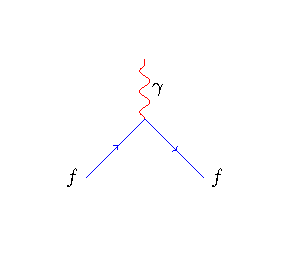
\includegraphics[width=0.5\textwidth]{qed_process}
  \caption[The elementary process for {QED}.] {The elementary process for {QED}
that all electromagnetic interactions can be reduced to, where $f$ is a charged
fermion and \Pphoton is a photon.}
  \label{fig:qed}
\end{figure}
The fine structure constant, $\alpha$, specifies the strength of the interaction
between charged particles and photon, and is given by
\begin{equation}
\alpha = \frac{e^2}{4 \pi} \approx \frac{1}{137}.
\end{equation}

The {Standard Model} describes all the interactions of known particles in terms
of gauge theories. A gauge theory is a theory that is invariant under a set of
gauge transformations.  In electromagnetism the gauge transformations are
complex phase transformations of the fields of the charged particles. Requiring local
gauge invariance will require that a massless vector particle be introduced, the
photon, that mediates the electromagnetic interaction.

The Lagrangian density for a free Dirac field, $\psi$, is given by,
\begin{equation}
\mathcal{L} = i \bar{\psi} \gamma_{\mu} \partial^{\mu} \psi - m \bar{\psi}\psi .
\end{equation}
This Lagrangian is invariant under a `global' phase transformation of the
fermion field,
\begin{align}
\psi(x)       &\to \psi^{\prime}(x) = e^{i\omega} \psi(x), \label{eq:global} \\
\bar{\psi}(x) &\to \bar{\psi}^{\prime}(x) = e^{-i\omega}\bar{\psi}(x),
\end{align}
where $\omega$ is a global arbitrary parameter. 
The Lagrangian is said to exhibit global gauge invariance. 

The family of transformations, $R = e^{i \omega}$, forms the
Abelian group $U(1)$ which is the group of all unitary $1\times 1$ matrices.
Unitary refers to the property that $U^{-1} = {U}^{\dagger}$.
Abelian refers to the property that all the elements in a
group commute, 
\begin{equation}
e^{-i\omega_1} 
e^{-i\omega_2} 
=
e^{-i\omega_2} 
e^{-i\omega_1} .
\end{equation}

If an infinitesimal transformation is considered then 
\begin{equation}
\psi(x) 
\to e^{i\omega} \psi(x)
\approx (1+i\omega)\psi(x),
\end{equation}
and it can be shown that the Lagrangian is unchanged by the
transformation\cite{halzen1984quarks}.

Global transformations introduce the problem that by making a transformation, it
is required that every space-time point must `know' about that transformation. It would be
preferable to require invariance under local transformations.
More generally, the \EquationRef{eq:global} can be rewritten as
\begin{equation}
\psi(x) \to e^{i\omega(x)} \psi(x),
\label{eq:local}
\end{equation}
where $\omega$ is now a function of the space time coordinate $x$. This is known
as a local phase transformation. The infinitesimal transformation now becomes,
\begin{equation}
\psi(x) 
\to e^{i\omega(x)} \psi(x)
\approx (1+i\omega(x))\psi(x),
\end{equation}
However, under this transformation the Lagrangian is now no longer
invariant \cite{halzen1984quarks}.
The gauge invariance can be restored if it is assumed that the fermion field
interacts with a vector field, called a gauge field and denoted $A_{\mu}$, with
an interaction,
\begin{equation}
-e\bar{\psi}\gamma^{\mu}A_{\mu}\psi
\end{equation}
where $A_\mu$ transforms under a gauge transformation as 
\begin{align}
-eA_{\mu} \to & -e\left(A_{\mu}+\delta A_{\mu}(x)\right)\\
           =   & -e A_{\mu} + \partial_{\mu} \omega (x)
\end{align}
and the new Lagrangian then becomes
\begin{align}
\mathcal{L} 
&= \bar{\psi}( i\gamma^{\mu} ( \partial_{\mu} +i e A_{\mu}) - m)\psi \\
&= \bar{\psi}( i\gamma^{\mu} D_{\mu} - m)\psi 
\end{align}
where the covariant derivative has been introduced,
\begin{equation}
D_{\mu} \equiv \partial_{\mu} + i e A_{\mu}.
\label{eq:covar_deriv}
\end{equation}
The vector field, $A_{\mu}$, couples with the electron, and can be identified as
the physical photon field. 

To complete the Lagrangian a kinetic term for the photon field should be added
which is quadratic in the derivative of the field.
However, this term should not break the invariance under gauge transformations.
This is achieved by defining the field strength tensor, $F_{\mu\nu}$,
\begin{equation}
F_{\mu\nu}
= \partial_{\mu} A_{\nu} - \partial_{\nu} A_{\mu}.
\label{eq:fieldstrengthtensor}
\end{equation}
which is gauge invariant. Therefore any term constructed only out of 
 $F_{\mu\nu}$ may be added to the Lagrangian.
A suitable term is $\frac{1}{4} F_{\mu\nu} F^{\mu\nu}$ which is quadratic in the
derivative of the field while remaining gauge invariant,
\begin{equation}
\mathcal{L} = \frac{1}{4} F_{\mu\nu} F^{\mu\nu} + \bar{\psi}( i\gamma^{\mu} D_{\mu} - m)\psi 
\end{equation}

Local gauge invariance has been restored with the introduction of the photon
field. An interesting result is that the photon is required to be massless, as
the introduction of a mass term for the photon, for example a term $\propto
A_{\mu}A^{\mu}$, will break the gauge invariance.

\subsection{Quantum Chromodynamics}
\label{sec:QCD}
The strong force is the force responsible for the interaction between particles
that carry a colour charge: quarks and gluons. Unlike the electric charge, the
colour charge can have three possible values, conventionally called `red',
`green' and `blue', as well as the corresponding anti-colour charges
`anti-red', `anti-green' and `anti-blue'.
The fundamental quark-gluon process of the strong force is shown in
\FigureRef{fig:qcdquark}.
\begin{figure}[htbp]
  \centering
  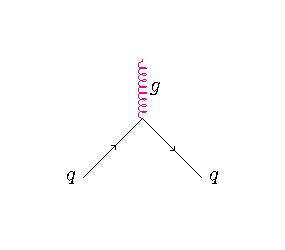
\includegraphics[width=0.5\textwidth]{qcd_process}
  \caption{The quark-gluon vertex for {QCD}.}
  \label{fig:qcdquark}
\end{figure}
The strong force is mediated by eight massless gluons which themselves carry
colour charge. This allows the gluons to self-interact which introduces gluon-gluon
vertexes in addition to the quark-gluon vertex which are shown in
\FigureRef{fig:qcd_gluon}.

\begin{figure}[htbp]
  \centering
  \begin{subfigure}{0.45\textwidth}
    \centering
    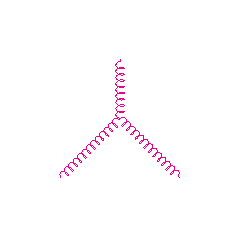
\includegraphics[width=\textwidth]{qcd_3gluon}
    \caption{Three-gluon vertex.}
    \label{fig:qcd_3gluon}
  \end{subfigure}
  \begin{subfigure}{0.45\textwidth}
    \centering
    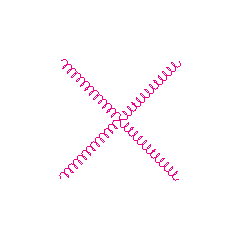
\includegraphics[width=\textwidth]{qcd_4gluon}
    \caption{Four-gluon vertex.}
    \label{fig:qcd_4gluon}
  \end{subfigure}
  \caption{Fundamental gluon-gluon vertices.}\label{fig:qcd_gluon} 
\end{figure}

The coupling constant for the strong force, $\alpha_s$, is given by,
\begin{equation}
\alpha_s = \frac{g_s^2}{4 \pi} \approx 1,
\end{equation}
which is approximately 100 times stronger than the {electromagnetic} force.

An interesting property of the strong force is that as the energy of the interaction
increases the strength of the strong coupling decreases. This is known as
asymptotic freedom; in high-energy experiments quarks appear to behave almost as
free particles. However, at lower energies the coupling increases and quarks
only appear in bound states. This phenomenon is known as quark confinement. 

The strong interaction is described by the theory of quantum chromodynamics
(QCD). QCD follows from similar reasoning to {QED}, but with
the Abelian $U(1)$ symmetry group replaced with the non-Abelian $SU(3)$ symmetry
group of transformations on the quark colour fields.

Quarks form colour triplets under $SU(3)$ transformations for each quark
flavour,
\begin{equation}
q_{f} =
\left(\begin{matrix} 
q^{red}_{f} \\
q^{green}_{f} \\
q^{blue}_{f} \\
\end{matrix} \right).
\end{equation}
The local gauge phase transformation under $SU(3)$ is given by,
\begin{equation}
q(x) \to e^{i\alpha_a(x)T_a} q(x),
\end{equation}
where $T_a$ are the generators of the $SU(3)$ group. The transformation breaks
the invariance of the Lagrangian. In a similar way to the U(1) transformation of
QED, the gauge invariance can be restored by introducing the covariant
derivative,
\begin{equation}
D_{\mu} \equiv \partial_{\mu} + i g T_{a} G_{\mu}^{a},
\end{equation}
where eight gauge fields have been introduced, instead of the single field in
QED.  The gauge fields transform as,
\begin{equation}
 G_{\mu}^{a} \to G_{\mu}^{a} 
-\frac{1}{g}\partial_{\mu}\alpha_{a}
-f_{abc}\alpha_{b}G^{c}_{\mu},
\end{equation}
where the last term has been added to produce a gauge invariant
Lagrangian due to the non-Abelian gauge transformation of $SU(3)$.

The final Lagrangian for QCD can now be written,
\begin{equation}
\mathcal{L} = 
\bar{q}(i\gamma^{\mu}\partial_{\mu} - m)q -
g \bar{q} \gamma^{\mu} G_{\mu}^{a} - 
\frac{1}{4} G_{\mu\nu}^{a} G^{\mu\nu}_{a},
\end{equation}
where the field strength tensor $G^{\mu\nu}_{a}$ is given by,
\begin{equation}
G^{\mu\nu}_{a} 
= \partial_{\mu} G^{a}_{\nu}
- \partial_{\nu} G^{a}_{\mu}
-g f_{abc} G^{b}_{\mu} G^{c}_{\nu}.
\end{equation}

In a similar way to QED, the Lagrangian for interacting coloured quarks, $q$, and
vector gluons, $G_{\mu}$, results from the simple requirement of local colour
phase invariance of the quark fields. Unlike the QED case, eight gauge fields
are needed due to the three quark colour fields.  Similar to QED, the gluons are
required to  be massless.

The field strength tensor, $G^{\mu\nu}_{a}$, introduces terms that are cubic and
quadratic in $G$. These represent three and four vertex gluon interactions
(\FigureRef{fig:qcd_gluon}) and are a result of the non-Abelian nature of the
$SU(3)$ group.

\subsection{Weak Force}
The weak interaction occurs between all fermions and is the interaction
responsible for the radioactive decay of sub-atomic particles.  Unlike the strong
and electromagnetic forces, the weak force is mediated by the exchange of
massive particles, the \PWpm and \PZ bosons, which cause the weak interaction
to have a very short range.

There are two kinds of weak interactions: charged and neutral, mediated by the
\PW and the \PZ respectively.

The fundamental vertex for the neutral interaction is shown in
\FigureRef{fig:neutral}, where the \PZ interacts with any left-handed quark or lepton.
The \PZ can mediate any process that can be mediated by the photon as well as
processes involving neutrinos.
\begin{figure}[htbp]
  \centering
  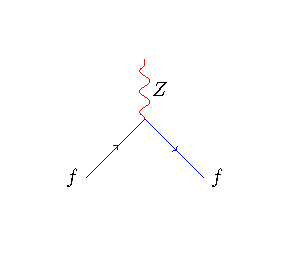
\includegraphics[width=0.5\textwidth]{weak_neut_process}
  \caption{The fundamental vertex of neutral weak interaction.\label{fig:neutral}}
\end{figure}
The fundamental vertices for the charged current are shown in
\FigureRef{fig:weak_charged}. The charged current has the unique ability to change the
flavour of quarks and leptons by the exchange of \PW bosons. The charged current
will only interact with fermions of the same generation
(\HepProcess{\Pelectron\to\Pnue} but never
\HepProcess{\Pelectron\to\Pnum}).

\begin{figure}[htbp]
  \centering
  \begin{subfigure}{0.45\textwidth}
    \centering
    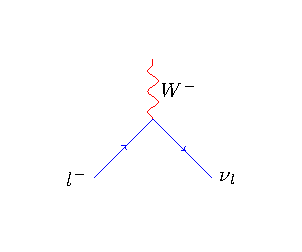
\includegraphics[width=\textwidth]{weak_charged_lepton_process}
    \caption{Leptons.}
    \label{fig:weak_charged_lepton_process}
  \end{subfigure}
  \begin{subfigure}{0.45\textwidth}
    \centering
    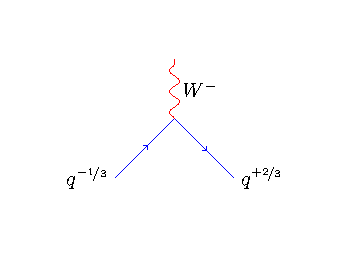
\includegraphics[width=\textwidth]{weak_charged_quark_process}
    \caption{Quarks.}
    \label{fig:weak_charged_quark_process}
  \end{subfigure}
  \caption{The fundamental vertices for charged weak interactions.}
  \label{fig:weak_charged}
\end{figure}

In a similar way to {QCD}, there is coupling of the \PW and \PZ bosons to one
another as shown in \FigureRef{fig:weak_boson}.

\begin{figure}[htbp]
  \centering
  \begin{subfigure}{0.3\textwidth}
    \centering
    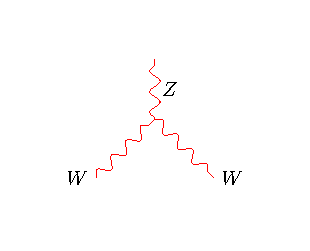
\includegraphics[width=\textwidth]{weak_WWZ}
    \caption{\HepProcess{\PW\PW\PZ}.}
    \label{fig:weak_WWZ}
  \end{subfigure}
  \begin{subfigure}{0.3\textwidth}
    \centering
    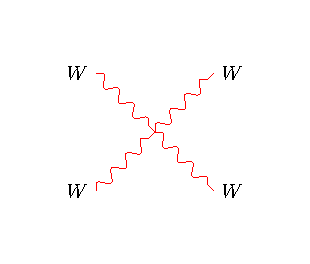
\includegraphics[width=\textwidth]{weak_WWWW}
    \caption{\HepProcess{\PW\PW\PW\PW}.}
    \label{fig:weak_WWWW}
  \end{subfigure}
  \begin{subfigure}{0.3\textwidth}
    \centering
    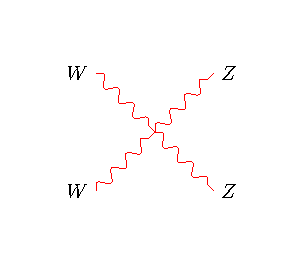
\includegraphics[width=\textwidth]{weak_WWZZ}
    \caption{\HepProcess{\PW\PW\PZ\PZ}.}
    \label{fig:weak_WWZZ}
  \end{subfigure}
  \caption{Direct couplings of the \PW and \PZ bosons to each other.}
  \label{fig:weak_boson}
\end{figure}

The weak interaction violates parity ($P$) and charge conjugation ($C$). A
well known example of parity violation in weak interactions is the Wu experiment
\cite{wu1957experimental}.
In the experiment, the $\beta$ decay of nuclei (Cobalt-60) polarised by an
external magnetic was studied, 
\begin{equation}
\begin{matrix}
\Rightarrow\Rightarrow \\
^{60}\mathrm{Co} \\
~   
\end{matrix}
\to
{^{60}\mathrm{Ni}}
+
\begin{matrix}
\Rightarrow \\
\Pelectron \\
\leftarrow 
\end{matrix}
+
\begin{matrix}
\Rightarrow \\
\APnue \\
\rightarrow 
\end{matrix},
\end{equation}
where the double arrows represent the spins and the single arrows represent the
direction of the particle produced in the decay.
The Cobalt-60 nuclei were aligned to the external magnetic field. By
conservation of angular momentum, the neutrino and electron spins must be
parallel and aligned with the magnetic field. By momentum conservation, the
electron and neutrino must be produced in opposite directions which means that
the electron and neutrino must have opposite helicity.  By changing the direction
of the magnetic field, the system undergoes a parity transformation
\begin{equation}
\begin{matrix}
\Leftarrow\Leftarrow \\
^{60}\mathrm{Co} \\
~   
\end{matrix}
\to
{^{60}\mathrm{Ni}}
+
\begin{matrix}
\Leftarrow \\
\Pelectron \\
\leftarrow 
\end{matrix}
+
\begin{matrix}
\Leftarrow \\
\APnue \\
\rightarrow 
\end{matrix}.
\end{equation}
If parity was conserved then the electron would have no preference in direction.
However, what was seen was that the electrons were preferentially emitted in the
opposite direction to their spin. The weak interaction exhibits maximal parity
violation.
More generally, the \PWpm boson is unique in that it only interacts with left-handed
particles (or right-handed antiparticles).

\subsection{Electroweak Interaction}
The electromagnetic and weak interactions can be described by a unified theory
known as the electroweak theory.
The gauge group for the electroweak theory is given by,
\begin{equation}
U(1)_{Y} \times SU(2)_{L} .
\end{equation}
The $L$ subscript on $SU(2)$ indicates that the weak force couples to the left
handed particles. 
The $Y$ indicates that the $U(1)$ group is not the gauge
group of QED but is that of the hypercharge which is connected to the electric
charge ($Q$) and the charge associated with the weak interaction, called weak
isospin ($I$), by the Gell-Mann-Nishijima relation,
\begin{equation}
Q = I_{3}+ \frac{1}{2}Y.
\end{equation}

The matter content of the theory are written as doublets or singlets. 
For the case of the leptons $l_{L}$ is a left
handed doublet,
\begin{equation}
l_{L} = \left( \begin{matrix} \nu \\ e \end{matrix} \right)_{L},
\end{equation}
and $e_{R}$ is a right-handed singlet.
For the case of the quarks, $q_{L}$ is a left-handed doublet,
\begin{equation}
q_{L} = \left( \begin{matrix} u\\ d \end{matrix} \right)_{L},
\end{equation}
and there are two right-handed singlets, the $u_{R}$ and the $d_{R}$.
In this description the left-handed fermions form isospin doublets and the right
handed fermions are singlets. Therefore, under $SU(2)_L$ gauge transformations,
\begin{align}
e_{R} &\to e_{R}^{\prime} = e_{R}\\
l_{L} &\to l_{L}^{\prime} = e^{-i \omega^{a} {T}^{a} }l_{L}
\end{align}
where $T^{a}$ are the generators of $SU(2)_L$.  The $SU(2)_L$ singlets are invariant
so do not couple with the corresponding gauge bosons.

The matter fields transform under the $U(1)_Y$ gauge transformations as,
\begin{equation}
\psi \to \psi^{\prime} = e^{-i\omega Y(\psi)}\psi
\end{equation}
where Y is the hypercharge of the particle.
\begin{equation}
Y(l_{L}) = -\frac{1}{2}, \qquad Y(e_{R}) = -1,
\end{equation}
\begin{equation}
Y(q_{L}) =  \frac{1}{6}, \qquad Y(u_{R}) =  \frac{2}{3}, \qquad Y(d_{R}) = -\frac{1}{3},
\end{equation}

The Lagrangian for the electroweak interaction can be written as the sum of the
gauge boson and the fermion parts,
\begin{equation}
\mathcal{L}_{electroweak} = 
\mathcal{L}_{fermion}
+ \mathcal{L}_{gauge}.
\end{equation}

The gauge part of the Lagrangian contains the kinetic terms and self interaction
terms for the gauge fields,
\begin{equation}
\mathcal{L}_{gauge} = 
- \frac{1}{4} B_{\mu\nu} B^{\mu\nu}
- \frac{1}{4} W^{a}_{\mu\nu} W^{a~\mu\nu}
\end{equation}
where the first term contains the hypercharge field strength and the second term 
contains the $SU(2)_L$ field strength where the index, $a$, runs from 1 to 3.
\begin{align*}
B^{\mu\nu}     &= \partial^{\mu} B^{\nu} - \partial^{\nu} B^{\mu},\\
W_{a}^{\mu\nu} &= \partial^{\mu} W_{a}^{\nu} - \partial^{\nu} W_{a}^{\mu} 
                + g \epsilon_{abc} W_{b}^{\mu} W_{c}^{\nu}.
\end{align*}

Four gauge fields have been introduced, 
three fields, ${W}^{a}_{\mu}$ , corresponding to the $SU(2)_{L}$
group and a single gauge field, $B_{\mu}$, corresponding to the $U(1)_{Y}$ group.
The physical $\PWp$ and $\PWm$ bosons are superpositions of the $W^{1}_{\mu}$
and $W^{2}_{\mu}$ gauge fields,
\begin{equation}
W^{\pm}_{\mu} = \frac{1}{\sqrt{2}} \left(W^{1}_{\mu} \mp W^{2}_{\mu}\right),
\label{eq:wgauge}
\end{equation}
and the photon and Z boson are combinations of the $B_{\mu}$ and $W^{3}_{\mu}$
gauge fields,
\begin{equation}
\left( \begin{matrix} A_{\mu}\\ Z_{\mu}\end{matrix}\right) =
\left( \begin{matrix} \cos\theta_{W} && \sin\theta_{W} \\  
                      -\sin\theta_{W} && \cos\theta_{W} \end{matrix}\right) 
\left( \begin{matrix} B_{\mu}\\ W^{3}_{\mu}\end{matrix}\right) ,
\label{eq:bgauge}
\end{equation}
where $\theta_{W}$ is the Weinberg angle which is related to the coupling
constants by
\begin{align*}
\sin\theta_{W} &= \frac{g^{\prime}}{\sqrt{g^{2}+{g^{\prime}}^{2}}},\\
\cos\theta_{W} &= \frac{g}{\sqrt{g^{2}+{g^{\prime}}^{2}}}.
\end{align*}

The fermion term has a lepton and a quark part,
\begin{equation}
\mathcal{L}_{fermion} =
 \mathcal{L}_{lepton}
+ \mathcal{L}_{quark}.
\end{equation}
The quark and lepton Lagrangians are given by,
\begin{align*}
\mathcal{L}_{lepton} &= 
\bar{l}_{L} i \gamma^{\mu} \mathbf{D}_{\mu} l_{L} +
\bar{e}_{R} i \gamma^{\mu} D_{\mu} e_{R}, \\
\mathcal{L}_{quark} &= 
\bar{q}_{L} i \gamma^{\mu} \mathbf{D}_{\mu} q_{L} +
\bar{u}_{R} i \gamma^{\mu} D_{\mu} u_{R} +
\bar{d}_{R} i \gamma^{\mu} D_{\mu} d_{R},
\end{align*}
where the covariant derivative has again been introduced.
The covariant derivative depends on the fermion field on which it acts. The covariant derivative
for the left-handed fermion, for example, is given by,
\begin{equation}
\mathbf{D}_\mu 
= \partial_\mu 
+ ig{T}^{a}W_{\mu}^{a}
+ ig^{\prime}Y(l^{L})B_{\mu},
\end{equation}
whereas the covariant derivative for the right-handed fermion, for example a
down quark, $d_R$, is given by, 
\begin{equation}
D_\mu = \partial_\mu + ig^{\prime}Y(d^{R})B_{\mu},
\end{equation}
where $g^\prime$ and $g$ and are the two coupling constants, ${T}^{a}$ are the
three generators of $SU(2)_L$ group and $W^{a}_{\mu}$ and $B_{\mu}$ are the four
gauge fields in the theory.

\subsubsection{Higgs Mechanism}

The Lagrangian, as it has been written so far, does not include terms for the
mass of any of the particles.  Adding in mass terms by hand will break the gauge
invariance rendering the theory meaningless \cite{ral}. 
Specifically, only a theory that is gauge invariant can be renormalised
\cite{t1972regularization}.

The symmetry needs to be broken in some natural way.  Spontaneous symmetry
breaking (SSB) is a method to break the symmetry by requiring that the Lagrangian of a
system remains invariant under a transformation, but the ground state is not
invariant.

An example of spontaneous symmetry breaking is a point mass in a potential,
\begin{equation}
V(r) = \mu^{2} \vec{r} \cdot \vec{r} + \lambda ( \vec{r} \cdot \vec{r} )^{2}
\end{equation}
where $\lambda$ is positive. This potential is radially symmetric. 
A point mass sits at $\vec{r}=0$. If $\mu^{2}>0$, as shown in
\FigureRef{fig:higgs_pot_mup} then $\vec{r}=0$ is the ground state and
the mass will remain at this point.
If $\mu^{2}<0$ then the potential will look like that given in
\FigureRef{fig:higgs_pot_mum}. The system remains symmetric, but $\vec{r}=0$ is no longer
the ground state. To fall to the ground state the mass has to ``choose'' a
direction to fall. The choice will break the symmetry of the system; the
potential remains symmetric, but the ground state is not. This is an example of
{SSB}.

\begin{figure}[htbp]
  \centering
  \begin{subfigure}{0.45\textwidth}
    \centering
    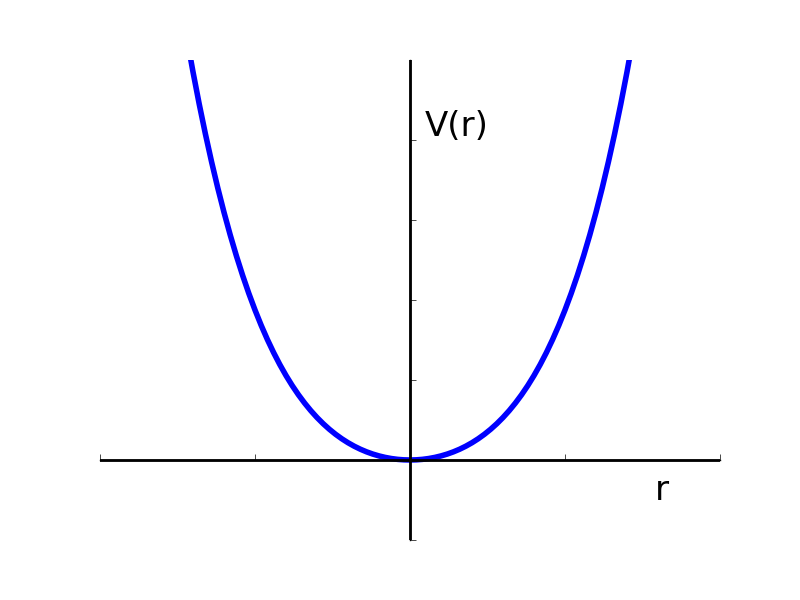
\includegraphics[width=\textwidth]{higgs_pot_mup}
    \caption{$\mu^{2}>0$.}
    \label{fig:higgs_pot_mup}
  \end{subfigure}
  \begin{subfigure}{0.45\textwidth}
    \centering
    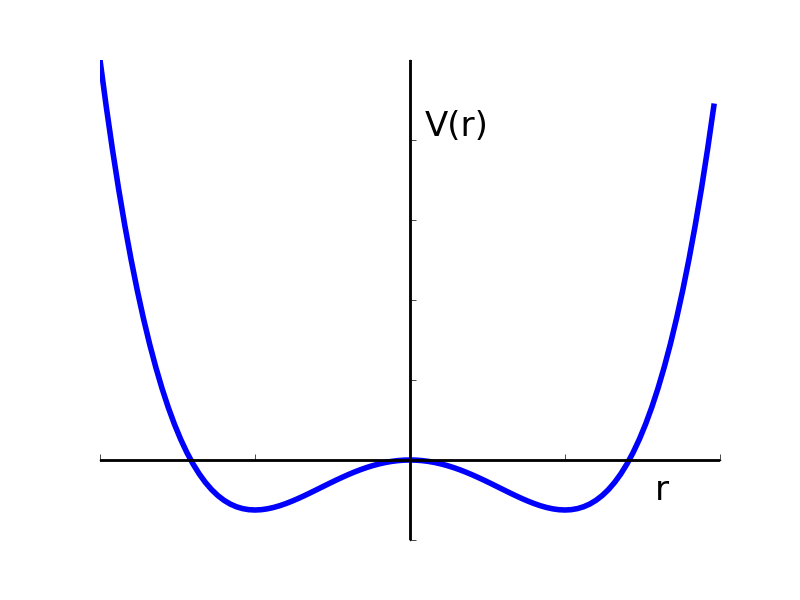
\includegraphics[width=\textwidth]{higgs_pot_mum}
    \caption{$\mu^{2}<0$.}
    \label{fig:higgs_pot_mum}
  \end{subfigure}
  \caption[The potential $ V(r) = \mu^{2} \vec{r} \cdot \vec{r} + \lambda (
\vec{r} \cdot \vec{r} )^{2}$.] {The potential $ V(r) = \mu^{2} \vec{r} \cdot
\vec{r} + \lambda ( \vec{r} \cdot \vec{r} )^{2}$. For simplicity, the potential
is shown for a single component of $\vec{r}$.}
  \label{fig:higgs_pot}
\end{figure}

The application of {SSB} to the {SM} was studied by Brout, Englert, Higgs
and others \cite{higgs1981broken, englert1964broken,
guralnik1964global,kibble1967symmetry}.
The result was a mechanism that spontaneously breaks the
 $SU(2)_{L} \times U(1)_{Y}$ symmetry called the Higgs mechanism\footnote{or the
Brout-Englert-Higgs mechanism, or even the
Englert-Brout-Higgs-Guralnik-Hagen-Kibble mechanism.}.

The Higgs mechanism introduces four real scalar fields, that can be arranged in
a complex doublet under $SU(2)$,
\begin{equation}
\Phi = \left( \begin{matrix} \phi^{+} \\ \phi^{0} \end{matrix} \right),
\end{equation}
where,
\begin{align*}
\phi^{+} &=\frac{1}{\sqrt{2}} (\phi_{1} + i \phi_{2}),\\
\phi^{0} &=\frac{1}{\sqrt{2}} (\phi_{3} + i \phi_{4}).
\end{align*}
The additional scalar part of the Lagrangian is,
\begin{equation}
\mathcal{L}_{scalar} = 
\left(D^{\mu}\Phi\right) \left(D_{\mu}\Phi\right) - V(\Phi),
\end{equation}
where the potential is,
\begin{equation}
V(\Phi) = 
\mu^{2}\Phi^{\dagger}\Phi + 
\lambda^{2} \left( \Phi^{\dagger} \Phi \right)^{2},
\end{equation}
where $\lambda$ and $\mu$ are free parameters. This Lagrangian is invariant
under $SU(2)_{L} \times U(1)_{Y}$ transformations.
By choosing  $\lambda>0$ and
$\mu^{2}<0$ there are minima at
\begin{equation}
\Phi^{\dagger} \Phi = \frac{- \mu^{2}}{2 \lambda}.
\end{equation}
The potential at $\Phi=0$ is unstable to small perturbations, and will fall
to a lower energy ground state. 
The ground state does not have the same symmetry as the Lagrangian; by
selecting a minimum the symmetry has become broken. An example choice of a minimum
could be,
\begin{equation}
\phi_{1} = \phi_{2} = \phi_{4} = 0,
\end{equation}
and
\begin{equation}
\phi_{3} = \frac{-\mu^{2}}{\lambda} \equiv v^{2}.
\end{equation}
which results in a non-zero vacuum-expectation value,
\begin{equation}
<0|\Phi|0> = \frac{1}{\sqrt{2}}\left(\begin{matrix}0\\v\end{matrix}\right),
\end{equation}
Fluctuations around the vacuum-expectation value can be 
parametrised in terms of the real scalar field, $H$,
\begin{equation}
\label{eq:phi}
\Phi = 
%\frac{1}{\sqrt{2}}
%e^{i\nicefrac{\sigma}{2}\phi_a}
%\left(\begin{matrix}0\\v+H\end{matrix}\right)
%\approx 
\frac{1}{\sqrt{2}}
\left(\begin{matrix}0\\v+H\end{matrix}\right)
\end{equation}
where $H$ is the physical Higgs field.  The Lagrangian can be now written in
terms of the $H$ field. The kinetic term,\cite{ral}
\begin{align}
\left(D_{\mu}\Phi\right) \left(D^{\mu}\Phi\right) 
&= \frac{1}{2} \left(\partial_{\mu}H\right) \left(\partial^{\mu}H\right) 
         + \frac{g^{2}v^{2}}{4} W_{\mu}^{+} W^{-~\mu} \nonumber \\
&\qquad{}+ \frac{g^{2}v^{2}}{8 \cos^{2}\theta_{W}} Z_{\mu} Z^{\mu} + 0 A_{\mu} A^{\mu} \nonumber \\
&\qquad{}+ \text{~ interaction terms},
\end{align}
now includes mass terms for the gauge bosons,
\begin{equation}
M_{W} = \frac{1}{2}gv, \qquad 
M_{Z} = \frac{1}{2}\frac{gv}{8\cos^{2}\theta_{W}} .
\end{equation}
while the photon remains massless, $M_{A}=0$.

The mechanism also introduces an additional boson with a mass
$\sqrt{-2\mu^{2}}$, called the Higgs boson.

\subsubsection{Fermion Masses and Yukawa Couplings}

Another feature of the Higgs mechanism is that it also provides a way to
introduce mass terms for the fermions, in a gauge invariant way, via the Yukawa
coupling between the leptons and the Higgs field. The Lagrangian for this
interaction for the electron can be written as, 
\begin{equation}
\mathcal{L}_{yukawa} = -Y_{e}\bar{l}_L\Phi e_R + h.c. \ ,
\end{equation}
where $Y_{e}$ is the coupling to the Higgs field known as the Yukawa coupling
and h.c. stands for the hermitian conjugate. On substitution of $\Phi$ (from
\EquationRef{eq:phi}), the Lagrangian for the Yukawa couplings becomes,
\begin{equation}
\mathcal{L}_{yukawa} = 
-\frac{Y_{e}}{\sqrt{2}} v
(\bar{e}_L e_R + \bar{e}_R e_L)
-\frac{Y_{e}}{\sqrt{2}}
(\bar{e}_L e_R + \bar{e}_R e_L)H
\end{equation}
and if $Y_e$ is chosen such that,
\begin{equation}
m_{e} = \frac{Y_{e}v}{\sqrt{2}}
\end{equation}
then the Lagrangian simplifies to,
\begin{equation}
\mathcal{L}_{yukawa} = 
- m_e \bar{e}e
- \frac{m_e}{v} \bar{e}e H
\end{equation}
which represents a mass term for the electron and a coupling of the electron to
the Higgs field proportional to the mass of the electron.
All fermion masses can also be generated in a similar way \cite{halzen1984quarks,ral}.

\subsubsection{Higgs Boson Observation}
On the fourth of July 2012, the two LHC experiments ATLAS and CMS both announced
the discovery of a new boson that is compatible with the Standard Model Higgs
boson \cite{aad2012observation,chatrchyan2012observation}. 

\begin{figure}[htbp]
  \centering
  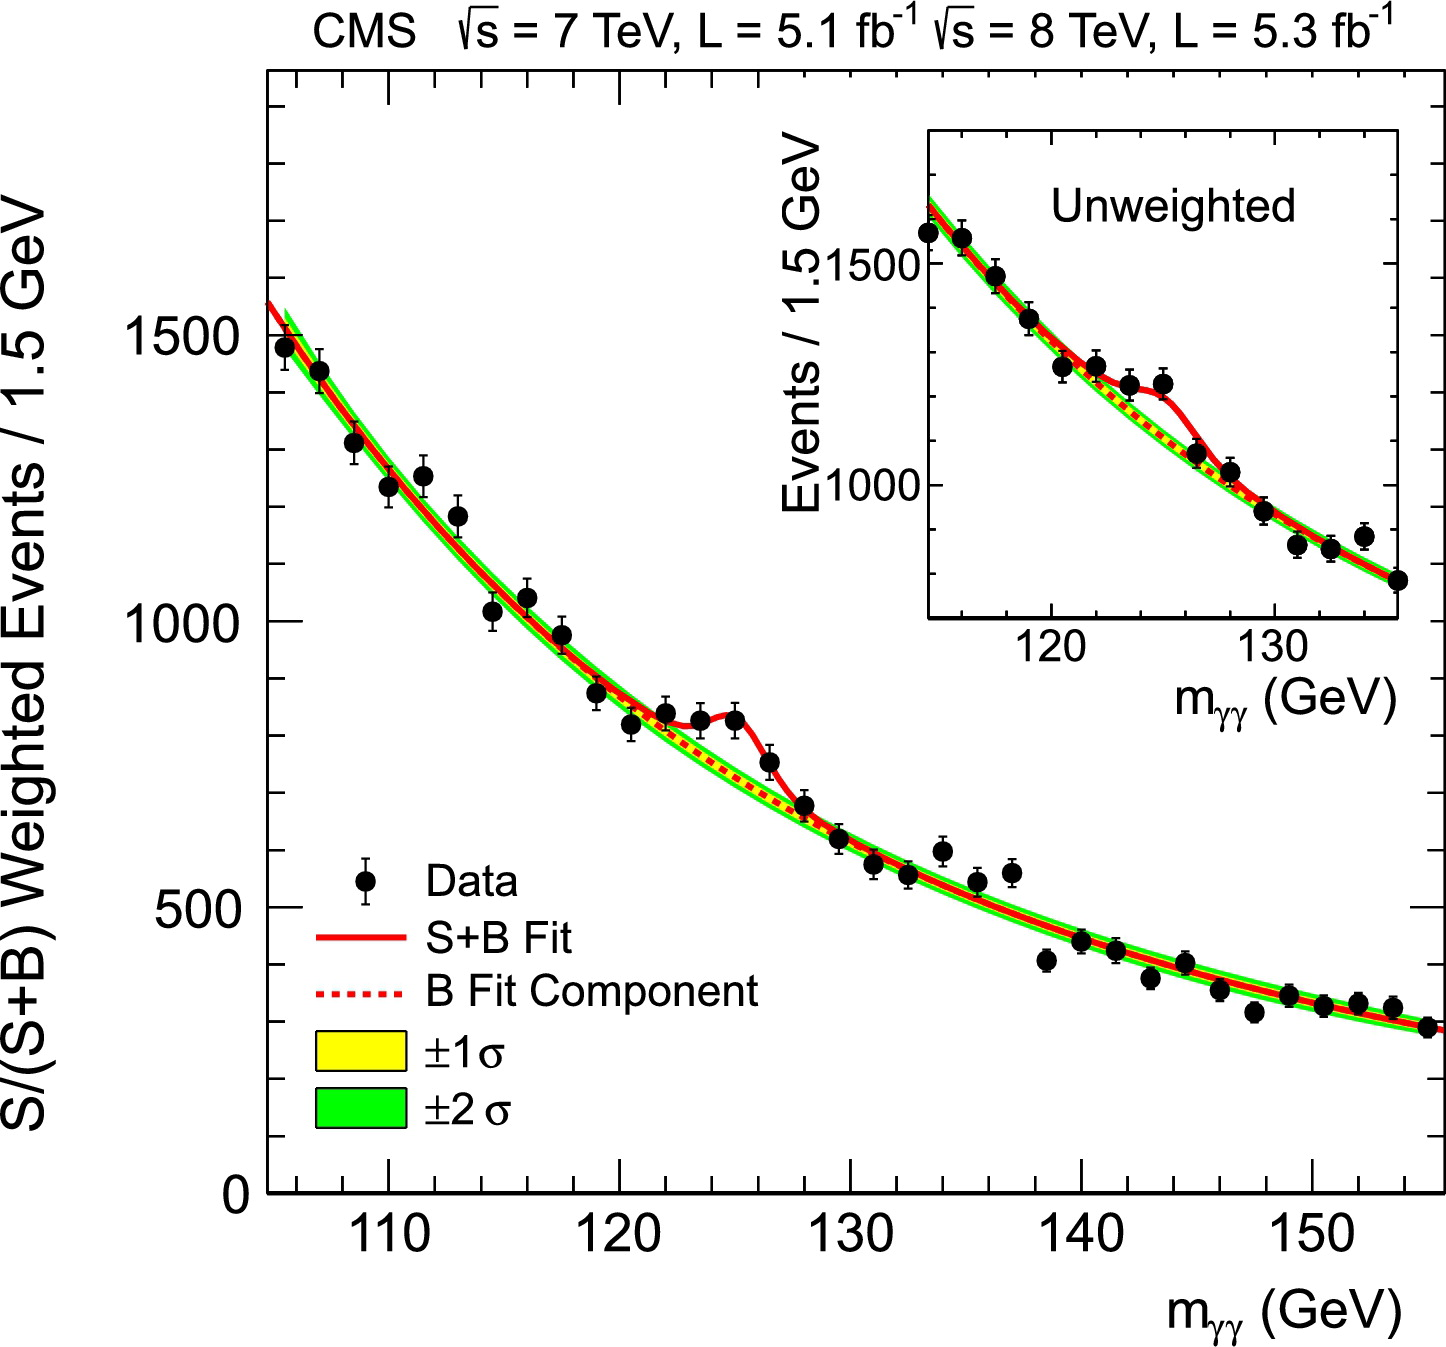
\includegraphics[width=0.8\textwidth]{higgs}
  \caption[The diphoton invariant mass distribution observed in CMS data.] {The
diphoton invariant mass distribution observed in CMS data.  Each event has been
categorised and then weighted by the S/(S + B) value of its category. The inset
is the unweighted invariant mass distribution. A peak in the region of
\unit{125}{\GeV} can clearly be seen. From \cite{chatrchyan2012observation}. }
  \label{fig:hgg}
\end{figure}

The Higgs search was performed in many different decay channels over a wide
mass range from 100 up to \unit{600}{\GeV}.
In the low-mass range, from 100 up to \unit{160}{\GeV}, a significant channel is the
diphoton channel, where the Higgs decays to a pair of photons via a top or \PW loop.
\FigureRef{fig:hgg} shows the diphoton invariant mass distribution measured in CMS.
A peak in the region of \unit{125}{\GeV} can clearly be seen. 
After combining the observations in each of the channels, an excess of events
was observed above what would be expected from only background events, with a
local significance of $\unit{5.0}{\sigma}$ at a mass near 125 GeV.


  \chapter{W Bosons at the LHC}
\label{chap:wboson}

\PW boson production is an important process for physics studies at the LHC, not
only for accurate measurements of the Standard Model, but also as a background
to many processes from new physics. 
At the {LHC}, \PW bosons are produced at a high rate while offering a clean
experimental signal with a final state consisting of, in the case of a
leptonically decaying \PW, a single high \PT lepton with a large amount of
missing transverse energy due to the neutrino in the event. 
The production of \PW bosons provides important
information on the interacting partons within the colliding
hadrons\cite{catani,kom}.

This chapter will first describe the asymmetric production of \PWp and \PWm bosons.
The next section will describe the leptonic decay of the \PW and describe the electron
charge asymmetry observable. The final section will show some theoretical
predictions of the electron charge asymmetry.

\section{W Boson Production}

The dominant production process for a \PW boson at a proton-proton collider is
given in \EquationRef{wbos:wprod},
and shown in \FigureRef{wbos:wproddiag}. 
\begin{equation}
  h_1(p_1) + h_2(p_2)
  \to 
  \PW + X
  \to
  \Plepton \Pnue + X.
  \label{wbos:wprod}
\end{equation}
The \PW boson is produced in the collision of a quark and an anti-quark from the
two incoming protons, $h_1$ and $h_2$, with momenta $p_1$ and $p_2$\footnote{In
this thesis, $p_1 = p_2 = \unit{3.5}{\TeV}. $}.  $X$ represents the accompanying
final state.

\begin{figure}[htbp]
  \centering
  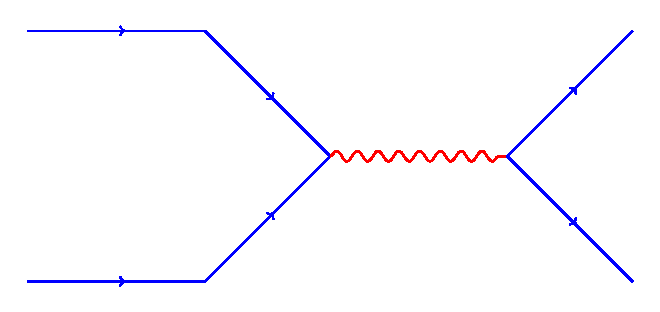
\includegraphics[width=0.6\textwidth]{w_production}
  \caption{Diagram of a W boson production and leptonic decay at a hadron-hadron collider.}
  \label{wbos:wproddiag}
\end{figure}

The \PW production cross section can given by the convolution of the cross
section at the parton level, and the parton distribution functions (PDF) of the
protons,
\begin{multline}
  d\sigma_{(\HepProcess{h_1 h_2 \to \PWpm})}(p_1,p_2;Q^{2}) = \\
  \sum\limits_{a,b}
  \int_0^1 \! \mathrm{d} x_1 
  \int_0^1 \! \mathrm{d} x_2 
  f_a^{h_1}(x_1,Q^2)
  f_b^{h_2}(x_2,Q^2) 
  d\hat{\sigma}_{(\HepProcess{a b \to \PWpm})}(x_1 p_1, x_2 p_2; Q^2),
  \label{wbos:xsec}
\end{multline}
where $\sum\limits_{a,b}$ represents the sum over the initial parton states $a$
and $b$, $f_a^{h}(x,Q^2)$ represents the proton {PDF} and
$d\hat{\sigma}_{(\HepProcess{a b \to \PWpm})}(x_1 p_1, x_2 p_2; Q^2)$
represents the partonic sub-process cross section. The ability to separate the
complicated QCD process in to a short-range perturbatively-calculable
hard-scattering process and long-range experimentally-measurable parton
densities is given by factorisation theorems. 
\todo{not sure this is enough}

\subsubsection*{Partonic Sub-Process}

At leading order (LO) the process for a \PWp is
\begin{equation}
  \HepProcess{\Pup + \APdown \to \PWp \to \Pleptonplus \Pnulepton} 
  \label{wbos:wpprod} 
\end{equation}
and for a \PWm:
\begin{equation}
  \HepProcess{\APup + \Pdown \to \PWm \to \Pleptonminus \APnulepton}
  \label{wbos:wmprod} 
\end{equation}
Tree-level Feynman diagrams representing these processes are shown in
\FigureRef{fig:w_process}.
At the {LHC} (a proton-proton collider), one parton is most to likely be a
valence quark with a high fraction of the proton's momentum, and the other
parton will tend to be a sea anti-quark with a lower fraction of the momentum
than the quark. The difference in momentum of the partons causes the \PW bosons 
to tend to be produced at high rapidities. 

\begin{figure}[htbp]
  \centering
  \begin{subfigure}{0.45\textwidth}
    \centering
    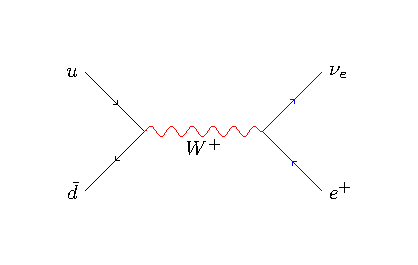
\includegraphics[width=\textwidth]{w_process_wp}
    \caption{\HepProcess{\Pup + \APdown \to \PWp \to \Pleptonplus \Pnulepton}}
    \label{fig:w_process_wp}
  \end{subfigure}
  \begin{subfigure}{0.45\textwidth}
    \centering
    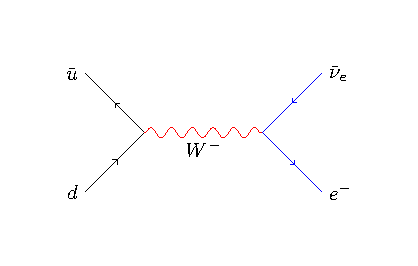
\includegraphics[width=\textwidth]{w_process_wm}
    \caption{\HepProcess{\APup + \Pdown \to \PWm \to \Pleptonminus \APnulepton}}
    \label{fig:w_process_wm}
  \end{subfigure}
  \caption{Tree-level diagrams for \PWp and \PWm boson production and electron
decay at a hadron-hadron collider.}\label{fig:w_process} 
\end{figure}

\subsubsection*{Proton Parton Distribution Function} 
The proton PDF represents the number density of
parton $a$ that has a fraction between $x$ and $x+\mathrm{d}x$ of the
momentum of the colliding hadron $h$ at a resolution scale $Q^{2}$.

\begin{figure}[htbp]
  \centering
  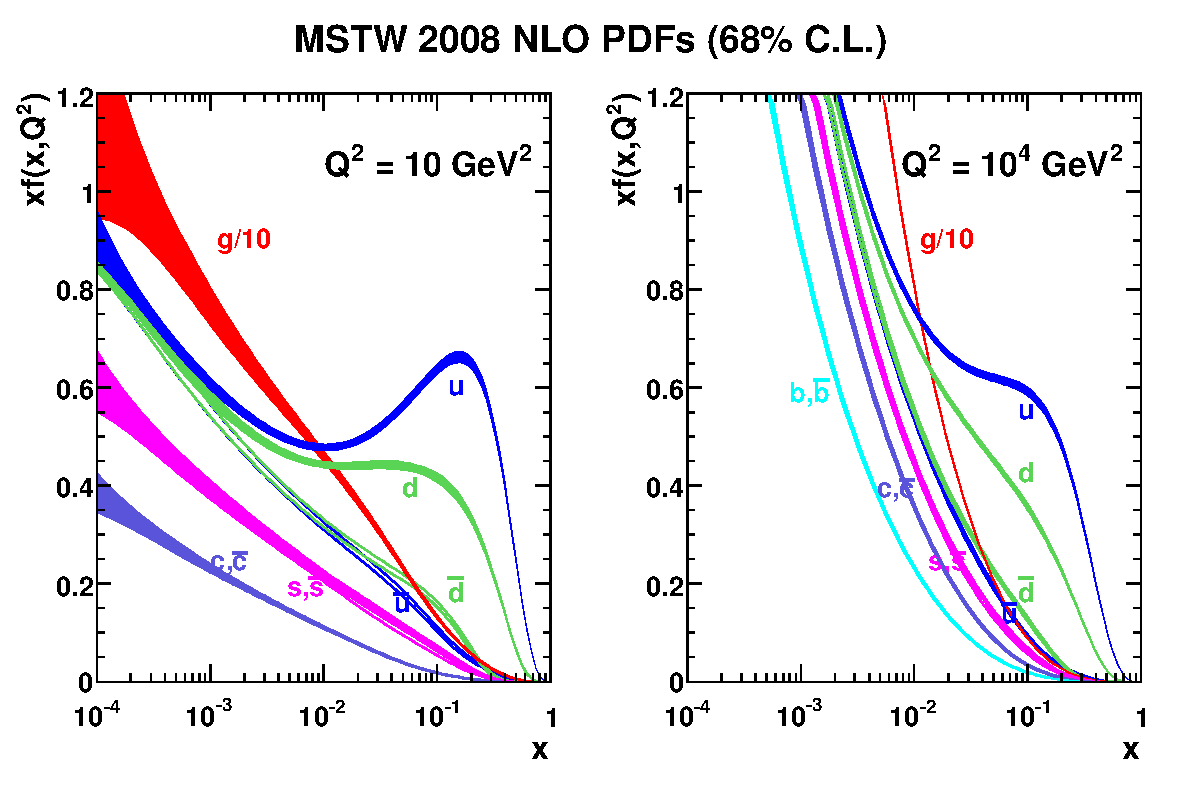
\includegraphics[width=\textwidth]{mstw2008nlo68cl_allpdfs}
  \caption
[Proton PDFs at $Q^2 = 10\ \GeV^2$ and $Q^2 = 10^{4}\ \GeV^2$.]
{Proton PDFs at $Q^2 = 10\ \GeV^2$ (left) and $Q^2 = 10^{4}\ \GeV^2$ (right) from \cite{martin2009parton}.}
  \label{wbos:pdf}
\end{figure}

The {PDFs} are obtained from global fits to experimental data
\cite{martin2009parton}.  \FigureRef{wbos:pdf} (right) shows the proton PDF at
$Q^2\approx M_{\PW}^2$ from the MSTW group.  The anti-quark parton densities
$\APup(x,Q^2)$ and $\APdown(x,Q^2)$ are relatively similar especially at the LHC
energies, where the parton momentum fraction, x, tends to be small.
However, the {PDF} for the valence quarks in the proton differ, 
the up-type quark dominates over the down-type quark.
This is due to the excess of up-type valence quarks with respect to down-type
valence quarks in the proton (\HepProcess{\Pup\Pup\Pdown}). 
This can be seen in the ratio of the up-type and the down-type {PDFs},
\begin{equation}
  R_{ud}(x,Q^2) = \frac{\Pup(x,Q^2)}{\Pdown(x,Q^2)} > 1,
\end{equation}
where $\Pup(x,Q^2)$ are the up and down quark {PDFs}.
\FigureRef{fig:pdf_plots} shows the ratio of the up-type and down-type quarks.
The ratio $R \approx 1$ for $x \ll 1$. This is due to the equal number or
up-type and down-type sea quarks in the proton. The equal number of sea quarks,
and the unequal number of valence quarks has the effect that if an up-type quark
is picked at random from the proton, it is more likely to be a higher momentum
valence quark, than if a down-type quark is picked.  Therefore, an up-type quark
will tend to have a greater fraction of the proton's momentum than a down-type
quark.

\begin{figure}[htbp]
  \centering
  %\begin{subfigure}{\textwidth}
    %\centering
    %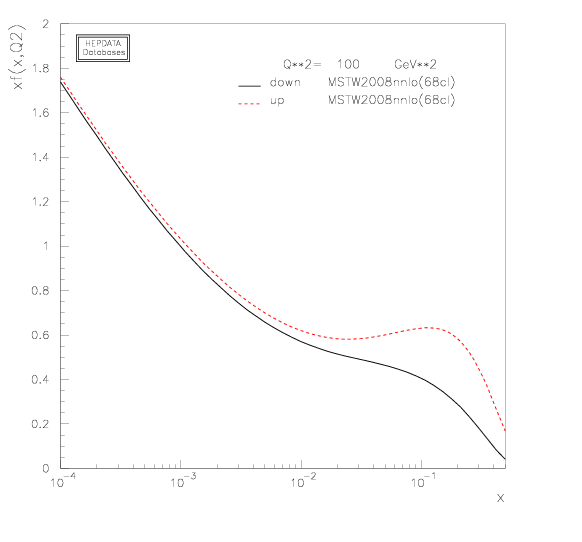
\includegraphics[width=0.75\textwidth]{plot_pdf}
    %\caption{PDF for \Pup and \Pdown}
    %\label{fig:plot_pdf}
  %\end{subfigure}
  %\begin{subfigure}{\textwidth}
    %\centering
    %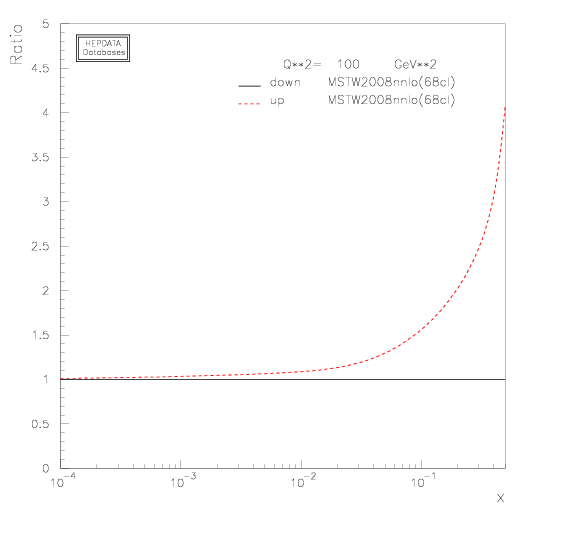
\includegraphics[width=0.75\textwidth]{plot_pdf_ratio}
    %\caption{Ratio for \Pup and \Pdown PDF}
    %\label{fig:plot_pdf_ratio}
  %\end{subfigure}
  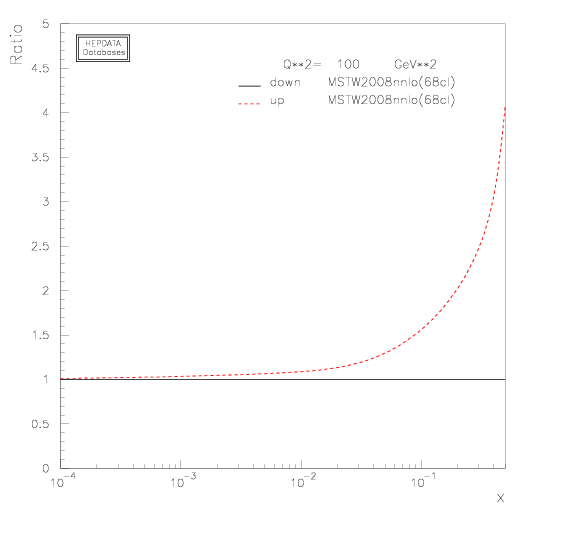
\includegraphics[width=0.75\textwidth]{plot_pdf_ratio}
  \caption[Ratio of up quarks to down quarks, $R_{ud}$ at $Q^2=\unit{100}{\GeV^2}$.] 
{Ratio of up quarks to down quarks, $R_{ud}$ at $Q^2=\unit{100}{\GeV^2}$.  Generated from \cite{hepdata} using the MSTW2008nlo
PDF sets \cite{martin2009parton}.}
  \label{fig:pdf_plots} 
\end{figure}

\subsection{\PW Boson Rapidity Distribution}
\label{wbos:wrapsec}

The rapidity of a particle is defined as,
\begin{equation}
    y = \frac{1}{2} \ln \left(\frac{E+p_\text{L}}{E-p_\text{L}}\right),
\end{equation}
where $p_{L}$ is the longitudinal component (the component along the beam axis)
of the momentum of the particle. It represents the boost along the beam axis
required to go from the lab frame to the frame where the particle is produced
perpendicular to the beam axis.
\begin{figure}[htbp]
  \centering
  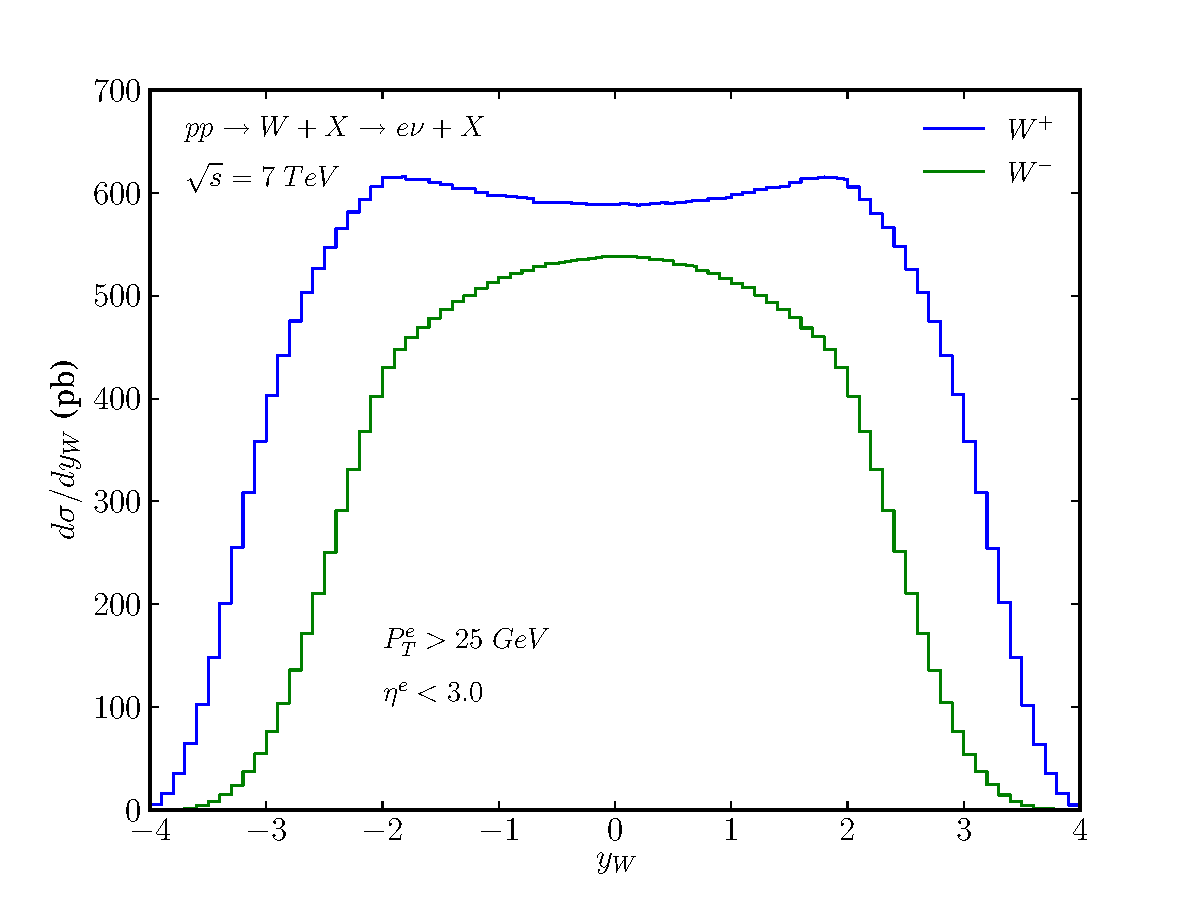
\includegraphics[width=0.8\textwidth]{w-rapidity}
  \caption[The rapidity distribution for \PWp and \PWm bosons in
${\sqrtS=\unit{7}{\TeV}}$ proton-proton collisions at the LHC.] {The rapidity
distribution for \PWp and \PWm bosons in $\sqrtS=\unit{7}{\TeV}$ proton-proton
collisions at the LHC.  Generated with the MSTW2008nlo
PDF set\cite{martin2009parton} interfaced with the MCFM generator tool \cite{campbellmcfm}.}
  \label{wbos:wrapid}
\end{figure}

The rapidity distributions, $y_W$, for \PWp and \PWm bosons produced at the
{LHC} are shown in \FigureRef{wbos:wrapid}.  The \PWp cross section is greater
than the \PWm cross section.  This is a consequence of the different production
processes for \PWp and \PWm bosons (shown in \EquationRef{wbos:wpprod} and
\EquationRef{wbos:wmprod} respectively) and the {PDF} for the valence quarks in
the proton differing as seen in \FigureRef{fig:pdf_plots}. The up-type quark
{PDF} dominates over the down-type which leads to a greater \PWp production rate
than \PWm.

It is also seen in \FigureRef{wbos:wrapid} that the \PWm tends to be produced
more centrally whereas the \PWp can be produced at larger rapidities. This is due
to up-type quarks tending to carry a greater fraction of the proton's momentum,
$x$, than the down-type quarks as seen in \FigureRef{fig:pdf_plots}.

The momentum fraction, $x$, of the interacting quarks is correlated with the
rapidity of the \PW boson. Therefore, the ratio of $\Pup$ and $\Pdown$ quarks as
a function of momentum fraction, $x$, is directly related to the difference in
the \PWp and \PWm production cross sections as a function of the boson rapidity.

Therefore a measurement of the asymmetric production of \PW bosons, as a
function of the rapidity of the boson, at the {LHC} provides important
information on the ratio of the up-type and down-type quark parton densities as
a function of $x$ ($R_{ud}(x,Q^2)$) within the proton\cite{kom}. 

\subsection{\PW Boson Charge Asymmetry}

The \PWpm boson charge asymmetry is defined as,
\begin{equation}
  A_{W}(y_{\PW})=
    \frac{ 
      \nicefrac{ d\sigma (\PWp) }{ dy_{W} } -
      \nicefrac{ d\sigma (\PWm) }{ dy_{W} }
    }
    {
      \nicefrac{ d\sigma (\PWp) }{ dy_{W} } +
      \nicefrac{ d\sigma (\PWm) }{ dy_{W} }
    }
,
\label{wbos:wasym}
\end{equation} 
where $y_{W}$ is the boson rapidity, and 
$\nicefrac{ d\sigma (\PWpm) }{ dy_{W} }$ is the \PWpm production cross section
at a fixed $y_{W}$.  
If $d\sigma(\PWp) > d\sigma(\PWm) $ then $A_{W}(y_{\PW})> 0$,
else if $d\sigma(\PWp) < d\sigma(\PWm) $ then $A_{W}(y_{\PW})< 0$,
and for symmetric \PWpm boson production, $A_{W}(y_{\PW})= 0$,

The prediction for the W boson charge asymmetry as a function of the boson
rapidity is shown in \FigureRef{wbos:chargeasym}. $A_{W}(y_{\PW})> 0$ and
increases as the rapidity increases.

\begin{figure}[htbp]
  \centering
  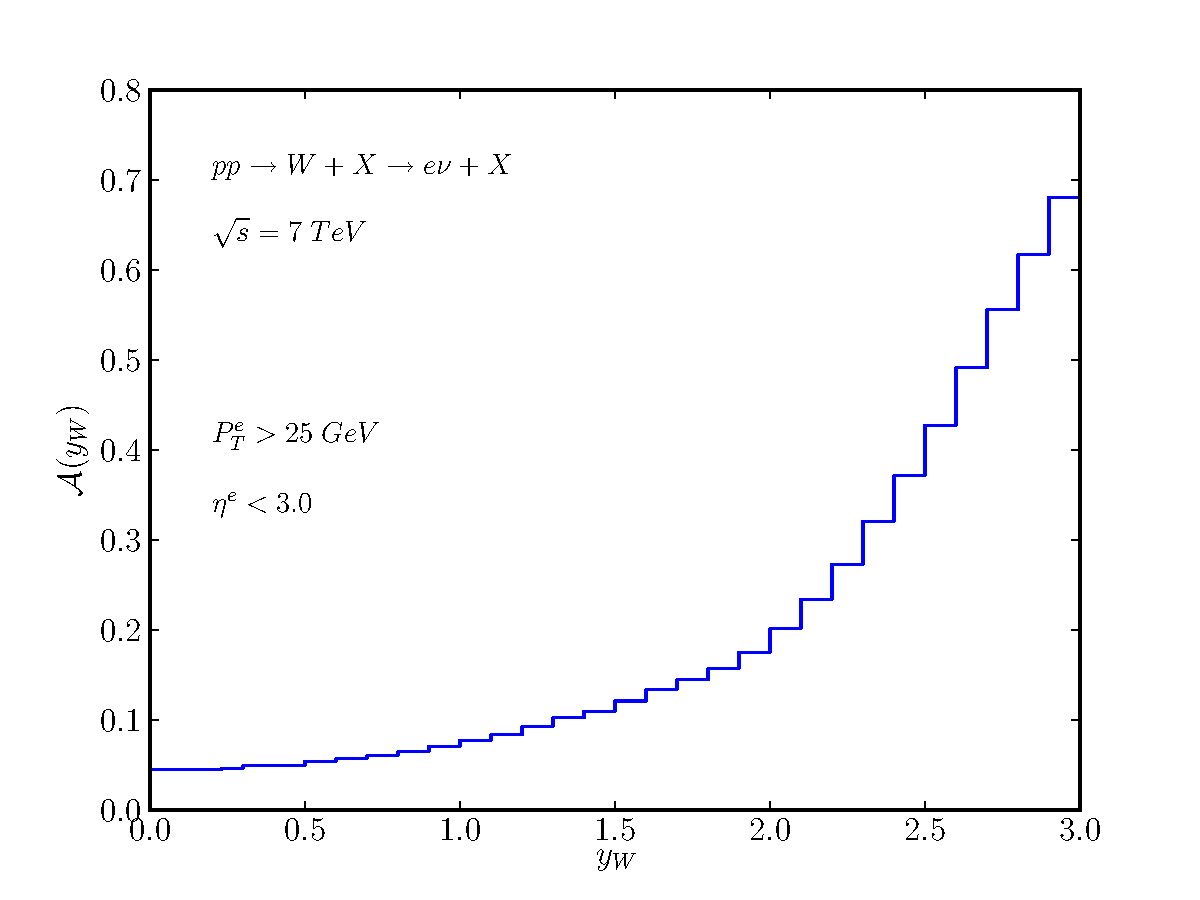
\includegraphics[width=0.8\textwidth]{w-asym}
  \caption[\PW boson charge asymmetry at LHC in ${\sqrtS=\unit{7}{\TeV}}$
proton-proton collisions.] {\PW boson charge asymmetry at LHC in
$\sqrtS=\unit{7}{\TeV}$ proton-proton collisions.  Generated with the
MSTW2008nlo PDF set\cite{martin2009parton} interfaced with the and the MCFM
generator tool \cite{campbellmcfm}.}
  \label{wbos:chargeasym}
\end{figure}

\PW bosons are identified by their decay to a lepton plus neutrino, however at
hadronic colliders the neutrino longitudinal momentum cannot be determined
which means that the \PW rapidity, $y_{W}$, cannot be measured.  Instead what
is studied is the charge asymmetry in the leptons that result from the \PW boson
decaying leptonically.

%It is possible to overcome the difficulty in determining the boson rapidity
%by extrapolating the neutrino longditudinal momentum from the lepton neutrino
%with a {MC} study. 

\section{W Boson Decay}
The \PW boson will decay to either a lepton and neutrino, or a pair of up and
down quarks. The branching fractions for the various decays are shown in
\TableRef{tab:w_decay}.
This thesis will consider the electron decay of the \PW boson which will occur
in approximately $11\%$ of \PW boson decays.

\begin{table}[htbp]
\begin{center}
\begin{tabular}{l l }
\toprule
\PWp Decay Mode & Fraction ($\Gamma_{i}/\Gamma$)\% \\
\midrule
\APelectron\Pnu & $10.75\pm0.13$ \\
\APmuon\Pnu     & $10.57\pm0.15$ \\
\APtauon\Pnu    & $11.25\pm0.20$ \\
hadrons         & $67.60\pm0.27$ \\
\bottomrule
\end{tabular}
\caption[Experimentally measured \PWp decay modes.] {Experimentally measured
\PWp decay modes. The decay modes of \PWm are the charge conjugates of the \PWp.
From \cite{beringer2012review}.\label{tab:w_decay}} 
\end{center}
\end{table}

\subsection{Electron Pseudorapidity Distribution}
The rapidity distributions of the charged leptons produced from \PWpm decay are
further complicated by the charge asymmetric decay of the \PWpm boson. 
The asymmetric decay arises due to the $V-A$ coupling of the \PW boson to the
annihilating \HepProcess{\Pquark\APquark} pair and the decaying lepton pair.

At leading order (LO) the \PWp is produced in the annihilation of a \Pup valance quark
with a \APdown sea-quark (\EquationRef{wbos:wpprod}). 
If the parton masses are neglected the \Pup is left-handed and the \APdown is
right-handed, as shown at the top of \FigureRef{wbos:wspin}. 

In the \PWp decay the \Ppositron is right-handed and the \Pnue is left-handed.
\FigureRef{wbos:wspin} shows that if the  positron is produced in the same direction
as the incoming \APdown quark angular momentum is conserved and the decay is
allowed.
However the decay where the positron is produced in the same direction as the
incoming \Pup quark is forbidden.
A similar argument holds true for \PWm decays, where the \Pelectron is produced
preferentially in the direction of the \Pdown quark.

\begin{figure}[htbp]
  \centering
  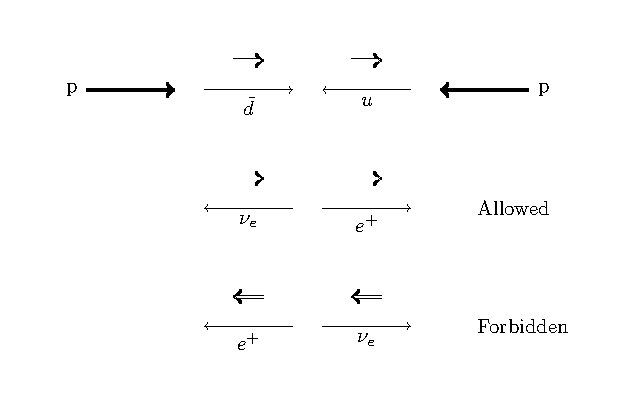
\includegraphics[width=0.8\textwidth]{w_decay_directions}
  \caption[Preferred directions of electron spins in
\HepProcess{\PWplus\to\APelectron\Pnue} decay.] {Preferred directions of
electron spins in \HepProcess{\PWplus\to\APelectron\Pnue} decay.  The heavy
arrows show the directions of the incoming protons, the thin arrows show the
directions of the incoming quarks and the outgoing electron and neutrino. The
double arrows show the spins.  Modified from \cite{aitchison2004gauge}. }
  \label{wbos:wspin}
\end{figure}

The distribution of the electron from \PWpm decay in the massless limit
is given by\cite{perkins2000introduction,aitchison2004gauge},
\begin{equation}
  \frac{1}{\sigma_{u\bar{d}}}
  \frac{d \sigma_{u\bar{d}}}{d \cos \theta_{\Plepton d}^{\ast}}
  =
  \frac{1}{\sigma_{d\bar{u}}}
  \frac{d \sigma_{d\bar{u}}}{d \cos \theta_{\Plepton d}^{\ast}}
  \propto
  (1+\cos \theta_{\Plepton d}^{\ast})^2
  \label{wbos:lepton}
\end{equation}
where $\theta_{\Plepton d}^{\ast}$ is the scattering angle of the charged
lepton with respect to the direction of the down-type quark or anti-quark, in
the centre of mass system of the two quarks. The cross section is maximised when
$\theta_{\Plepton D}^{\ast}$ is minimised and the charged lepton is produced in
the same direction as the down-type quark.

The rapidity distribution of the electron is therefore a convolution of the
{electroweak} correlations in \EquationRef{wbos:lepton} with the \PW rapidity
described in \SectionRef{wbos:wrapsec}.  In proton-proton collisions the \PWp
tends to be produced in the direction of the \Pup.  However, due to the
electroweak correlations the charged lepton from the decaying \PWp will tend to
be produced along the direction of the down-type quark and therefore will shift
the rapidity distribution of the lepton to be more central. Similarly, \PWm
bosons tend to be produced more centrally, however the electroweak correlations
will shift the charged lepton rapidity distribution to higher rapidities.

\FigureRef{fig:leptonrapidity} shows the Monte Carlo (MC) generated
pseudorapidity distribution of electrons and positrons produced in
$\sqrtS=\unit{7}{\TeV}$ proton-proton collisions.  
The pseudorapidity is defined as 
\begin{equation}
    \eta = -\ln\left[\tan\left(\frac{\theta}{2}\right)\right], 
\end{equation}
where $\theta$ is the polar angle.  In the massless approximation, the
pseudorapidity of the electron is equal to the rapidity.

\begin{figure}[htbp]
  \centering
  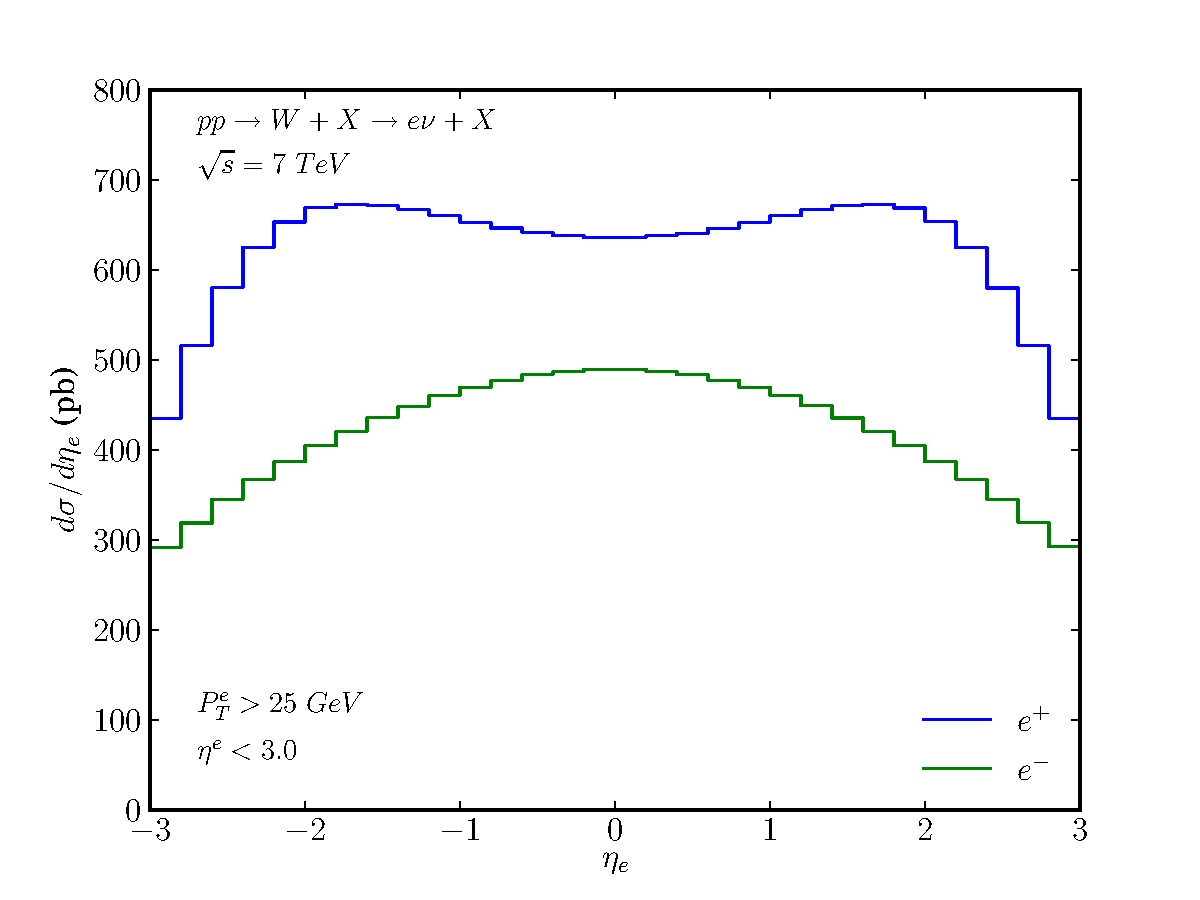
\includegraphics[width=0.8\textwidth]{lepton-rapidity}
  \caption[Electron and positron pseudorapidity, $\eta_e$, distributions in
$\sqrtS=\unit{7}{\TeV}$ proton-proton collisions.] {Electron and positron
pseudorapidity, $\eta_e$, distributions in $\sqrtS=\unit{7}{\TeV}$ proton-proton
collisions. Generated with the MSTW2008nlo PDF set\cite{martin2009parton}
interfaced with the MCFM generator tool \cite{campbellmcfm}.}
  \label{fig:leptonrapidity}
\end{figure}

\subsection{Electron Charge Asymmetry}

The electron asymmetry is defined in \EquationRef{eq:AsymThe} analogously to the
\PW boson asymmetry in \EquationRef{wbos:wasym}, as the difference in the
\HepProcess{\PWplus \to \APelectron} and \HepProcess{\PWminus \to \Pelectron}
over the total \inclusiveWe cross section.
\begin{equation}
A_{the}(\eta)=\frac
  { \frac{d\sigma}{d\eta}(\Wpenu) - \frac{d\sigma}{d\eta}(\Wmenu) }
  { \frac{d\sigma}{d\eta}(\Wpenu) + \frac{d\sigma}{d\eta}(\Wmenu) }
\label{eq:AsymThe}
\end{equation} 

The electron charge asymmetry has previously been studied in $p\bar{p}$
collisions by the CDF and D0 experiments at the Fermilab Tevatron collider
\cite{cdfWAsym,d0WAsym}. 

\FigureRef{wbos:asym_simple} shows the electron charge asymmetry prediction for
electron transverse momentum cuts of \unit{25}{\GeV}. The prediction was
produced using the MSTW2008NLO PDF\cite{martin2009parton} set.
Unlike the \PW asymmetry, the electron asymmetry turns over at $\eta\approx
2.25$. This effect is due to the electroweak correlations in the leptonic decay of
the \PW boson.

\begin{figure}[htbp]
  \centering
  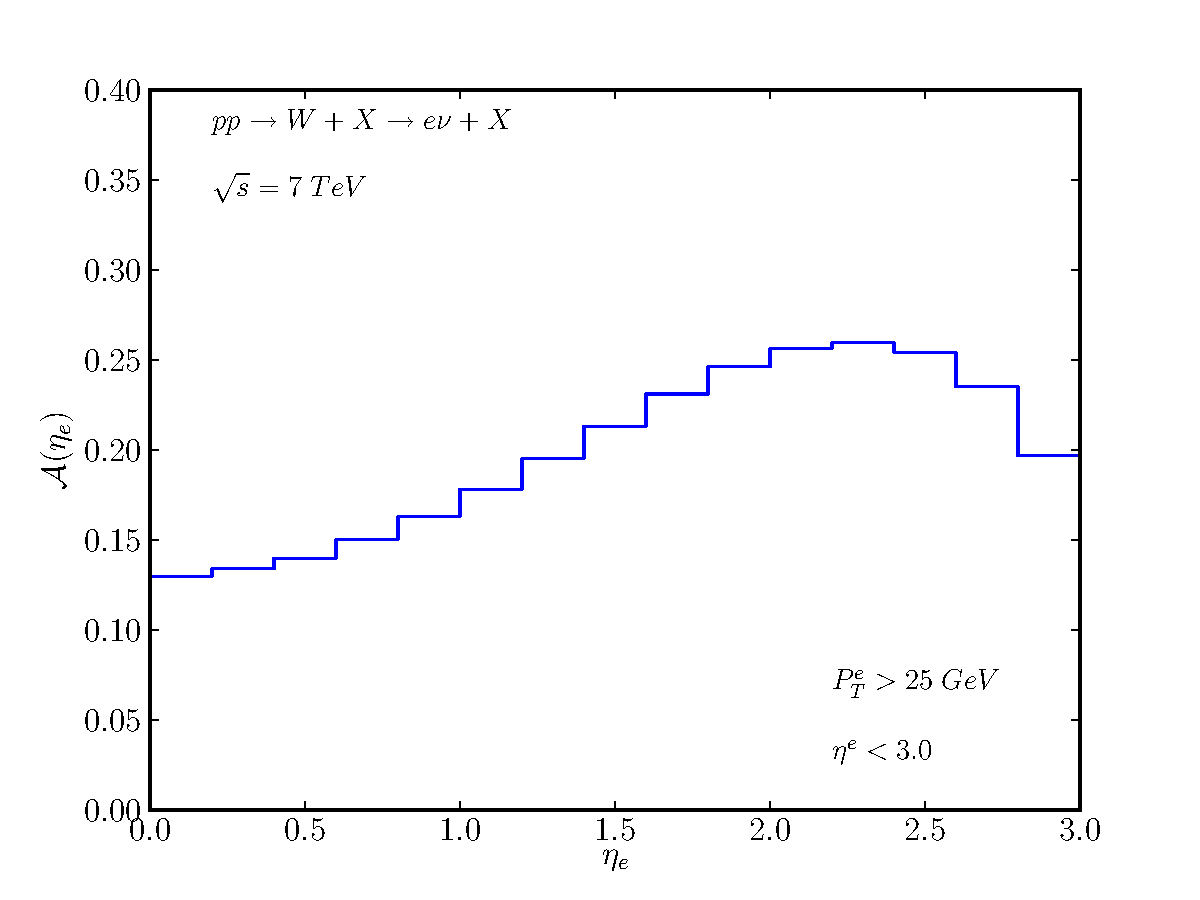
\includegraphics[width=0.8\textwidth]{lepton-asym}
  \caption[Electron charge asymmetry at LHC in ${\sqrtS=\unit{7}{\TeV}}$
proton-proton collisions.] {Electron charge asymmetry at LHC in
$\sqrtS=\unit{7}{\TeV}$ proton-proton collisions.  Generated with the
MSTW2008nlo PDF set\cite{martin2009parton} interfaced with the MCFM generator tool
\cite{campbellmcfm}.}
  \label{wbos:asym_simple}
\end{figure}

In an experiment, the cross section is not measured directly, instead what is
measured are the electron and positron yields.  The experimentally measured
asymmetry is given by \EquationRef{eq:AsymExp},
\begin{equation}
A_{exp}(\eta)=\frac{  \frac{dN}{d\eta}(\APelectron) -
\frac{dN}{d\eta}(\Pelectron)}{\frac{dN}{d\eta}(\APelectron) +
\frac{dN}{d\eta}(\Pelectron)}
\label{eq:AsymExp}
\end{equation} 

To get from the experimentally measured asymmetry to the lepton charge
asymmetry, \EquationRef{eq:NumEve} must be used, which takes into
account the experimental effects such as the luminosity (${\cal L}$), high
level trigger ($\epsilon_{HLT}$), offline efficiency ($ \epsilon_{off}$) and
the acceptance ($\epsilon_{acc}$).

\begin{equation}
\frac{dN}{d\eta} = {\cal L } \frac{d\sigma}{d\eta}  \epsilon_{HLT}
\epsilon_{off} \epsilon_{acc}
\label{eq:NumEve}
\end{equation} 
As the asymmetry is a ratio, the luminosity, high level trigger and the
offline efficiency can be cancelled out assuming that they are not asymmetric
with respect to charge. 

The acceptance cannot be cancelled, it is a function of transverse momentum of
the electron, and these distributions will differ for \Pelectron and \APelectron.
A correction due to acceptance effect could be included, but would be highly
dependent on the choice of PDF set used to generate the corrections \cite{cdfWAsym}.
The measurements presented in this thesis do not correct for acceptance effects.

%\begin{align} 
%A_{exp}(\eta) &= \frac{ \frac{dN}{d\eta}(\Pelectron) -
%\frac{dN}{d\eta}(\APelectron) }{\frac{dN}{d\eta}(\Pelectron) +
%\frac{dN}{d\eta}(\APelectron) }\\   
              %&= \frac{ \frac{d\sigma}{d\eta}(\Wpenu) -
%\frac{\epsilon^{-}_{acc}}{\epsilon^{+}_{acc}} \frac{d\sigma}{d\eta}(\Wmenu) }{
%\frac{d\sigma}{d\eta}(\Wpenu) + \frac{\epsilon^{-}_{acc}}{\epsilon^{+}_{acc}}
%\frac{d\sigma}{d\eta}(\Wmenu) }
%\label{eq:AsymExpCorr}
%\end{align}

\section{ Theoretical Predictions of the Electron Charge Asymmetry }
\label{sec:asymuncert}

In this section predictions for the electron charge asymmetry are investigated in
detail.  The predictions are calculated using the MCFM\cite{campbellmcfm} {MC} tool
interfaced with the LHAPDF package\cite{whalley2005houches}.  LHAPDF provides an
interface to many different {PDF} sets. For the following predictions, PDF sets from
the MSTW \cite{martin2009parton} and CTEQ \cite{lai2010vv} collaborations are
used.

Corrections for final state radiation (FSR) are not included in the predictions.
In the measurements presented in the later chapters, FSR in considered as an
additional contribution to the electron energy resolution and is corrected for, so the
comparison of the measured asymmetry to the theoretical predictions is valid.

\subsection{Uncertainty on Theoretical Predictions}
The theoretical predictions of the electron charge asymmetry will have an error
associated with the uncertainty on the {PDF}.
The uncertainty on the {PDF} originates from the experimental errors on the
data used in the global fits performed by each of the {PDF} collaborations.

Each {PDF} collaboration produces a set of {PDFs} that include the
central value, or best fit to experimental data, and $2N$ error {PDFs}, where
$N$ is the number of free parameters used in the global
fit\cite{Bourilkov:2006cj}.
For each of the free parameters there is a PDF produced with the parameter at its upper
error and another with the parameter at its lower error. 

The uncertainty on the observable, in this case the lepton asymmetry, is found
by producing $2N+1$ theoretical predictions, one for each member of the {PDF}
set. The predictions are then used to approximate the {PDF} uncertainty by
using the `master equation'\cite{Bourilkov:2006cj,campbell2006hard}.
For the upper uncertainty,

\begin{equation}
\Delta A^{+}_{max}
= \sqrt{ \sum^{N}_{i=1} \left[ max( A^{+}_i-A_{0}, A^{-}_i-A_{0}, 0 ) \right]^{2}}
\end{equation}
and for the lower uncertainty,
\begin{equation}
\Delta A^{-}_{max}
= \sqrt{ \sum^{N}_{i=1} \left[ max( A_{0}-A^{+}_i, A_{0}-A^{-}_i, 0 ) \right]^{2}}
\end{equation}
where $A^{\pm}_{i}$ is the asymmetry prediction using the {PDF} with the
positive/negative fluctuation of parameter $i$ and $A_{0}$ is the prediction
using the central value.

\subsection{Prediction of the Electron Charge Asymmetry above \unit{25}{\GeV}}

\begin{figure}[htbp]
  \centering
  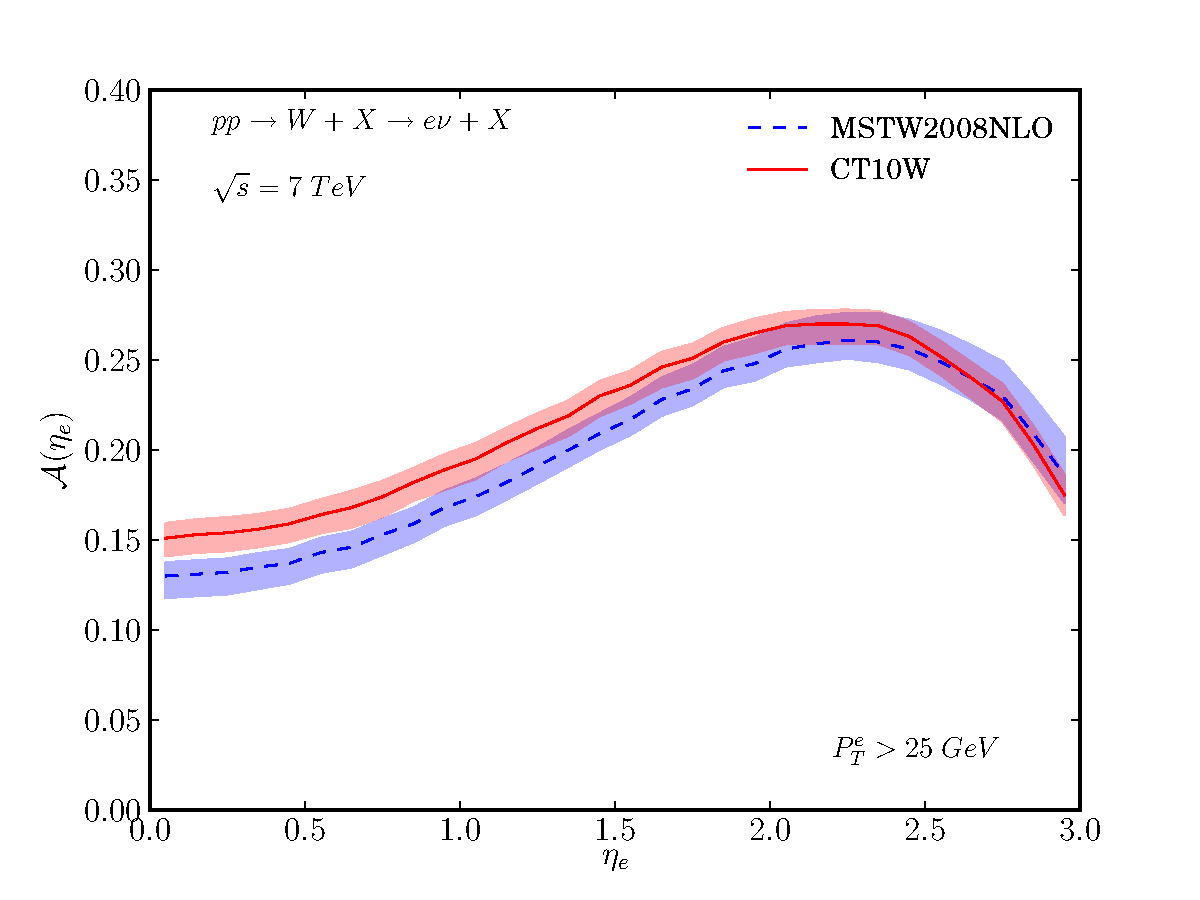
\includegraphics[width=0.8\textwidth]{asym-uncert}
  \caption[The theoretical electron charge asymmetry for a ${\pT>\unit{25}{\GeV}}$
with the {PDF} uncertainties.] {The theoretical electron charge
asymmetry\cite{monchenault2011predictions} for a $\pT>\unit{25}{\GeV}$ with the
{PDF} uncertainties for the MSTW08NLO\cite{martin2009parton} and
CT10W\cite{lai2010vv} {PDF} sets. The uncertainties are $68\%$ confidence level. The
predictions are generated using the {MCFM} \cite{campbellmcfm} generator.}
  \label{fig:asym-uncert}
\end{figure}

\FigureRef{fig:asym-uncert} shows the theoretical predictions for the electron
charge asymmetry for $\pT>\unit{25}{\GeV}$ with PDF sets from the MSTW
collaboration\cite{martin2009parton} and the CTEQ collaboration\cite{lai2010vv}.
The uncertainty due to the PDFs is included.  The predictions show a
disagreement at low rapidities. The CTEQ prediction tends to be higher and the
MSTW prediction lower. The disagreement is greater than the PDF uncertainty on
the prediction.

\subsection{Prediction of the Electron Charge Asymmetry above \unit{30}{\GeV}}

\begin{figure}[htbp]
  \centering
  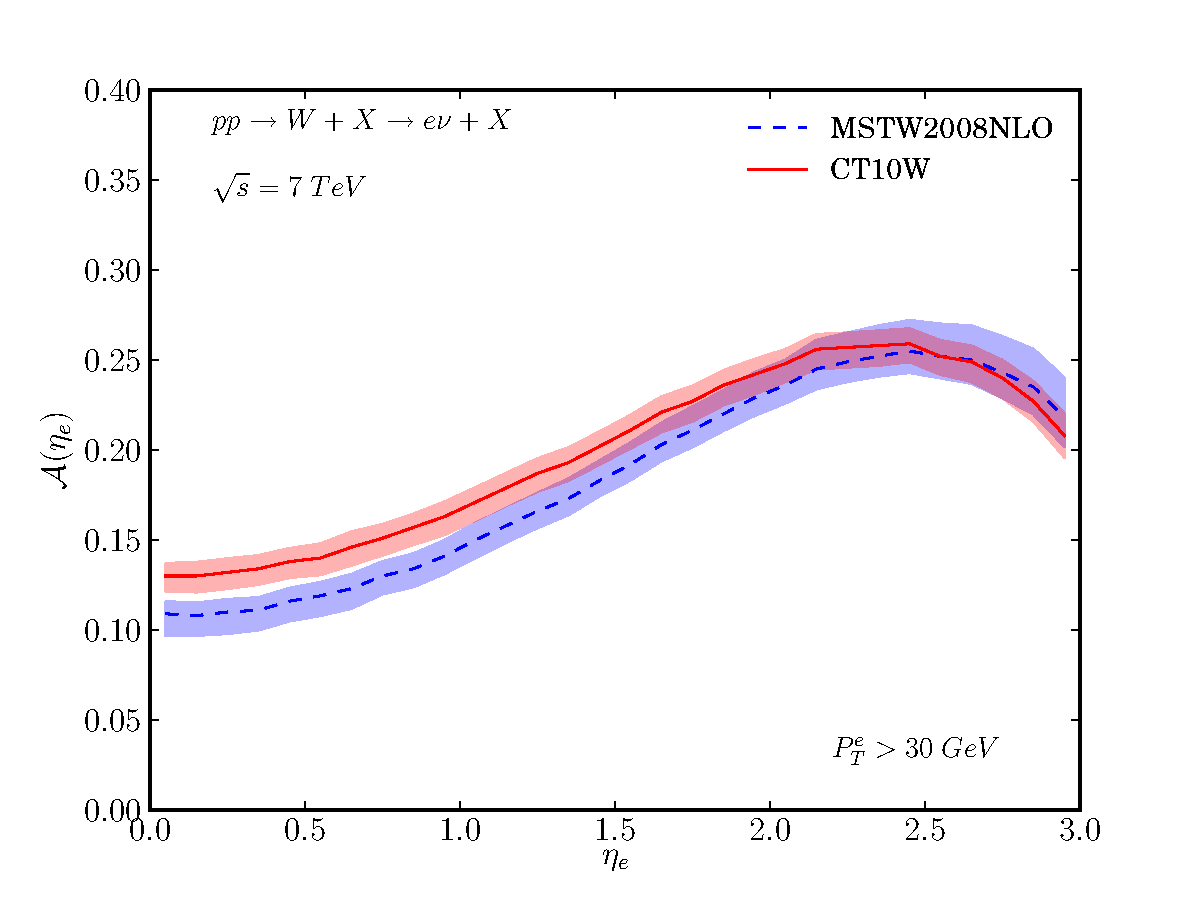
\includegraphics[width=0.8\textwidth]{asym-uncert-30}
  \caption[The theoretical electron charge asymmetry for a ${\pT>\unit{25}{\GeV}}$
with the {PDF} uncertainties.] {The theoretical electron charge
asymmetry\cite{monchenault2011predictions} for a $\pT>\unit{30}{\GeV}$ with the
{PDF} uncertainties for the MSTW08NLO\cite{martin2009parton} and
CT10W\cite{lai2010vv} {PDF} sets. The uncertainties are $68\%$ confidence level. The
predictions are generated using the {MCFM} \cite{campbellmcfm} generator.}
  \label{fig:asym-uncert-30}
\end{figure}

\FigureRef{fig:asym-uncert-30} shows the theoretical predictions for the
electron charge asymmetry for $\pT>\unit{30}{\GeV}$ with PDF sets from the MSTW
collaboration\cite{martin2009parton} and the CTEQ collaboration\cite{lai2010vv}.
Similar disagreement between the predictions at low rapidities is seen.

The asymmetry prediction at low rapidities is lower than the prediction with an
electron cut at \unit{25}{\GeV}. The turning point in the asymmetry is also
shifted to higher rapidities.




  \chapter{The LHC and the CMS Detector}
\label{chap:LHC}
\section{Large Hadron Collider}
The Large Hadron Collider (LHC)\cite{lhc} is a circular synchrotron with a
circumference of \unit{27}{\kilo\meter}.  It has been constructed in the
existing tunnel \unit{40-170}{\meter} beneath the border of France and
Switzerland that was previously home to the LEP collider \cite{myers1990design}.

When operating at its design energy and luminosity it will collide beams of
protons at a centre of mass energy of \unit{14}{\TeV} and a luminosity of
\unit{$10^{34}$}{\rpsquare\cm\reciprocal\second}.  It is also designed to
collide two \unit{5.5}{\TeV} beams of lead ions, and other species\cite{lhc}.
\TableRef{tab:lhcparam} summarises the machine parameters relevant to the {CMS}
detector.

\begin{table}[htbp]
\begin{center}
\begin{tabular}{ l l l }
\toprule
Parameter & p-p & Pb-Pb \\
\midrule
Energy per nucleon ($\TeV$)& 7 & 2.36 \\
Dipole field at \unit{7}{\TeV} ($\tesla$)& 8.33 & 8.33\\
Design luminosity ($\lumiunits$)& $10^{34}$ & $10^{27}$ \\
Bunch separation ($\ns$)& 25 & 100\\
No. of bunches & 2808 & 592 \\
No. particles per bunch& $1.15\times10^{11}$ & $1.15\times10^{11}$\\
\midrule
$\beta$-value at IP ($\metre$)& 0.55 & 0.5 \\
RMS beam radius at IP ($\micron$)& 16.7 & 15.9 \\
Luminosity lifetime (hr)& 15 & 6 \\
Average number of collisions/crossing & 20 & - \\
\bottomrule
\end{tabular}
\caption[The machine parameters relevant for the LHC detectors.]
{The machine parameters relevant for the LHC detectors. From \cite{chatrchyan2008cms}.}
\label{tab:lhcparam}
\end{center}
\end{table}

The main motivation for the LHC is to determine the mechanism that is
responsible for electroweak symmetry breaking, of which the most favoured is the
Higgs mechanism.  The LHC is also designed to test the Standard Model at the
$\TeV$ scale at high precision and to search for new particles predicted by
theories beyond the Standard Model such as supersymmetric theories and theories
involving extra dimensions.  \FigureRef{fig:LHCxsec} shows various cross
sections for several physics processes as a function of the centre of mass
energy. The cross section for many physics processes of interest, such as the
Higgs cross section, $\sigma_{Higgs}$, are many orders of magnitude lower than the
total inelastic cross section, $\sigma_{tot}$, and increase as a function of
centre of mass energy.  The large centre of mass energy and high luminosity of
the LHC is needed to be able to probe the physics processes of interest with
small cross sections.

\begin{figure}[htbp]
  \centering
  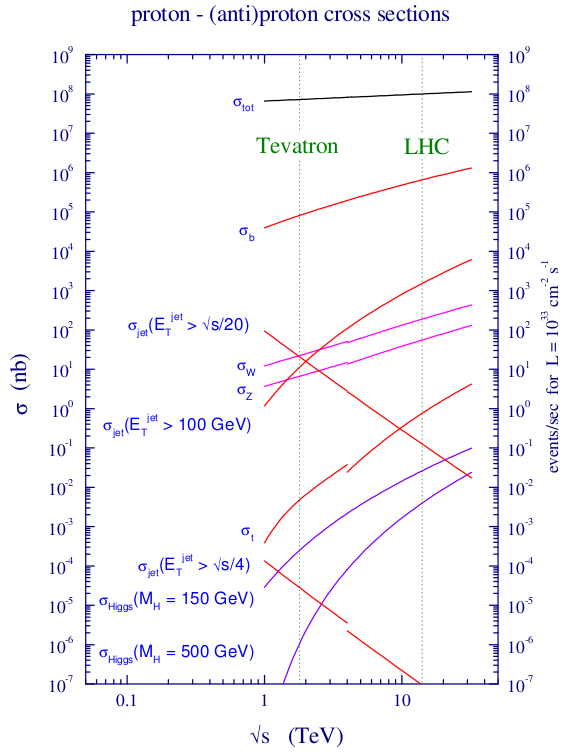
\includegraphics[width=0.85\textwidth]{xsec.png}
  \caption[The theoretical production cross sections as a function of centre of
mass energy for several Standard Model processes.] {The theoretical production
cross sections as a function of centre of mass energy for several Standard Model
processes such as the b quark production cross section, $\sigma_{b}$, and the
Higgs boson production cross sections, $\sigma_{Higgs}$.  $\sigma_{tot}$ is the
total inelastic cross section.  The cross sections that are of relevance to this
thesis analysis are the \PW and \PZ boson cross sections $\sigma_{\PW}$ and
$\sigma_{\PZ}$ respectively.  From \cite{campbell2006hard}.}

  \label{fig:LHCxsec}
\end{figure}

The LHC is part of a larger accelerator complex as shown in 
\FigureRef{fig:LHCcomplex}. Hydrogen gas is first ionised to produce a cloud of
protons, which are then accelerated by the LINAC2 linear accelerator to
\unit{50}{\MeV}.  Before being injected into the Proton Synchrotron (PS) the
protons are injected into the Proton Synchrotron Booster (PSB) and accelerated
to \unit{1.4}{\GeV}. In the PS the protons are grouped into bunches and the
energy is increased to \unit{25}{\GeV}. The bunches are then accelerated in the
Super Proton Synchrotron (SPS) to \unit{450}{\GeV} and then injected into the
LHC.

\begin{figure}[htbp]
  \centering
  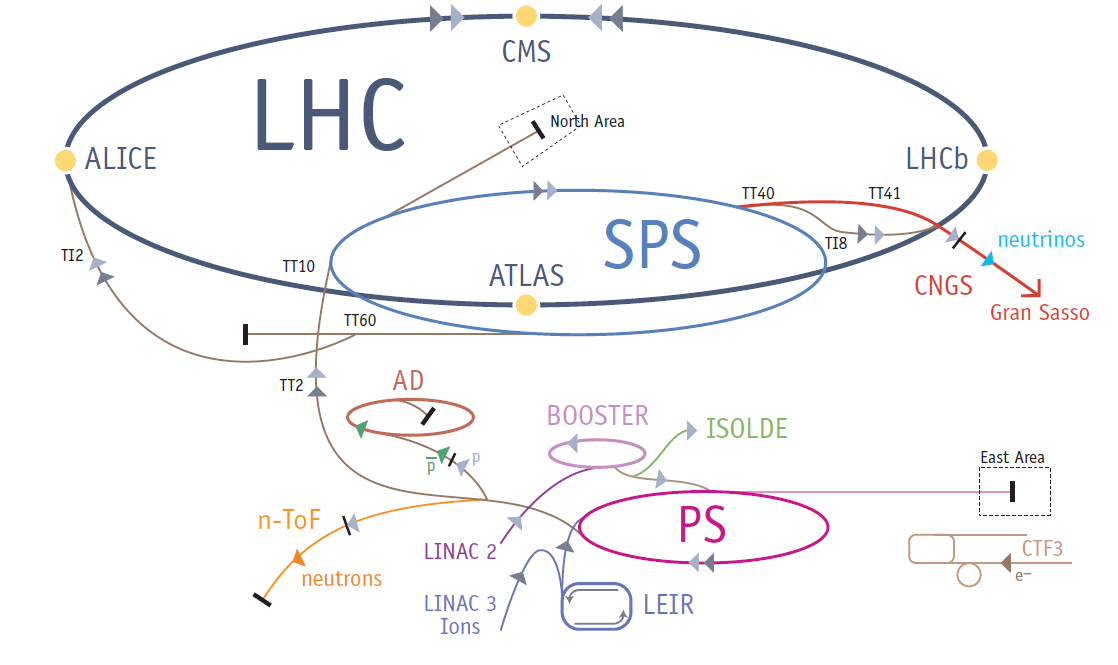
\includegraphics[width=0.96\textwidth]{accelerators.png}
  \caption{The LHC complex.}
  \label{fig:LHCcomplex}
\end{figure}

There are four main experiments studying the collisions at the
{LHC}.  
ALICE\footnote{A Large Ion Collider Experiment.} is designed to study the quark
gluon plasma that will be produced in the heavy ion collisions
\cite{aamodt2008alice}.
The LHCb\footnote{Large Hadron Collider beauty.} experiment is designed to study
B-meson decays to measure CP violation \cite{alves2008lhcb}.
ATLAS\footnote{A Toroidal LHC Apparatus.} and CMS\footnote{Compact Muon
Solenoid.} are general purpose detectors that are designed to search for a wide
range of new physics \cite{chatrchyan2008cms,aad2008atlas}.

In addition there are two smaller special-purpose detectors.
The LHCf \footnote{Large Hadron Collider forward.} is an experiment designed to
measure the neutral particles emitted in the very forward region of LHC
collisions.  The goal of the experiment is to provide data for hadron
interaction models that are used in the study of extremely high-energy
cosmic-rays \cite{adriani2008lhcf}.
The goal of the TOTEM\footnote{TOTal Elastic and diffractive cross section
Measurement.} experiment is to measure the total proton-proton
cross section and study the elastic and diffractive scattering at the LHC. The
detector is located at either side of the CMS detector \cite{anelli2008totem}.

\subsection{Operational History}
In September 2008 the {LHC} was commissioned and the first beams were
circulated.  Before the first collisions could be delivered an interconnection
between two of the dipole magnets failed. This led to
a large amount to helium rapidly evaporating which caused considerable damage to
the machine \cite{lebrun2009sector}.  Due to this incident it was decided that,
after the repairs,
the {LHC} should be run at a lower centre of mass energy of \unit{7}{\TeV} until
the quench protection system could be upgraded and the interconnections
thoroughly verified for higher currents \cite{myers2010lhc}.

The {LHC} was repaired by the end of 2009 and the first collisions at a record
energy of \unit{2.36}{\TeV} were delivered in November.  From March to November
2010 the {LHC} operated at \unit{7}{\TeV} delivering \unit{46.4}{\invpb} of
proton-proton collisions of which \unit{36.1}{\invpb} was certified for analysis
\cite{myers1990design}.  In November and December 2010 the {LHC} produced lead
ion collisions at \unit{2.36}{\TeV}.

\begin{figure}[htbp]
  \centering
  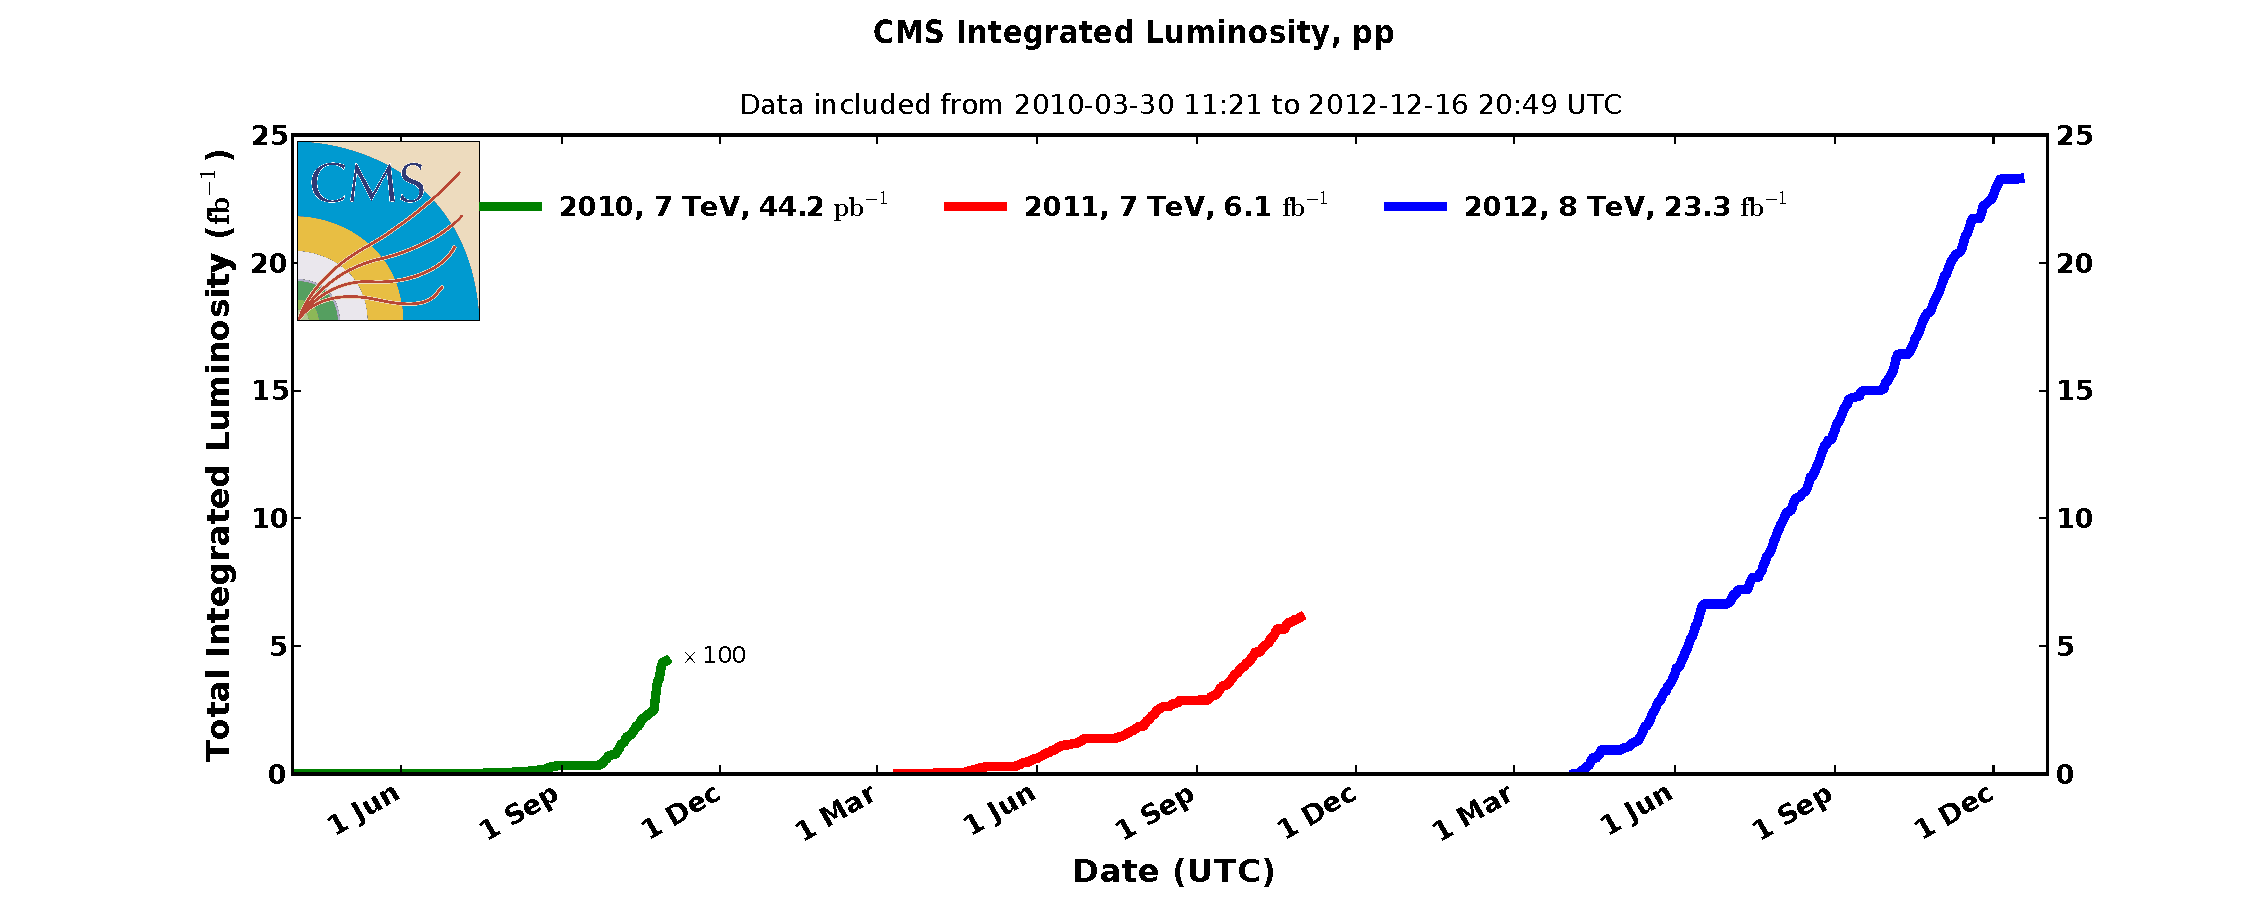
\includegraphics[width=\textwidth]{int_lumi_cumulative_pp_1}
  \caption[The luminosity delivered by LHC and recorded by CMS in 2010, 2011 and
2012.] {The luminosity delivered by LHC and recorded by CMS in 2010, 2011 and
2012. From \cite{intlumi}.}
  \label{fig:LHC2010}
\end{figure}

The target for running in 2011 was to deliver \unit{1}{\invfb} of data. This was
achieved by June. The target was increased to \unit{5}{\invfb} of data for 2011 which was achieved by October. 
In 2012 the {LHC} was operated at a centre of mass energy of \unit{8}{\TeV}
and a total of \unit{22.1}{\invfb} of data was collected by December.
The luminosity delivered by LHC and recorded in CMS in 2010, 2011 and 2012 is
shown in \FigureRef{fig:LHC2010} \cite{intlumi}.

The analysis presented in the following chapters is based on the
\unit{36.1}{\invpb} of data from  2010 and \unit{840}{\invpb} of data from the first half of 2011.

\section{CMS Detector}
{CMS}\cite{chatrchyan2008cms} is one of the two general purpose
detectors designed to study LHC collisions. The main design parameters for the
{CMS} detectors  are listed in \TableRef{tab:cmsparam}.

\begin{table}[htbp]
\begin{center}
\begin{tabular}{ l l }
\toprule
Parameter & CMS \\
\midrule
Total weight (tons)                 & $12,500$  \\
Overall diameter (m)                & $15$  \\
Overall length (m)                  & $20$  \\
Magnetic field for tracking (T)     & $4$  \\
Solid angle for energy measurements ($\Delta\phi \times \Delta\eta$)   
                                    & $2\pi \times 9.6$  \\
Solid angle for precision measurements ($\Delta\phi \times \Delta\eta$)   
                                    & $2\pi \times 5.0$  \\
Total cost (CHF)                    & $550\times 10 ^{6}$  \\
\bottomrule
\end{tabular}
\caption[Main design parameters of the CMS detector.]{Main design parameters of
the CMS detector. From \cite{froidevaux2006general}.\label{tab:cmsparam}}
\end{center}
\end{table}

The design goals of the CMS detector are:
\begin{itemize}
  \item Good muon identification and momentum resolution and the ability to
unambiguously assign charge to muons with $\PT < \unit{1}{\TeV}$
  \item Good charged particle momentum resolution and reconstruction in the
tracker.
  \item Good electromagnetic energy resolution. 
  \item Good resolution of missing transverse energy and dijet mass.
\end{itemize}

The design of CMS meets these requirements while overcoming significant
experimental challenges.  At design luminosity, approximately 1 billion
inelastic events will occur in CMS every second, whereas CMS is limited to
storing the data of only $\approx 100 $ events within that time.  The detector
must be able to reduce this rate with a trigger to accept events that are
interesting from a physics perspective and reject events otherwise.

In addition to this challenge, each event of interest will have on average 20
inelastic events superimposed on it. This results in around 1000 charged
particles produced every \unit{25}{\ns}, which require the detectors to
have a high granularity with a good time resolution to ensure a low occupancy.
The large flux of particles will also produce high radiation levels which 
required radiation hard detectors and electronics.

\begin{figure}[htbp]
  \centering
  \includegraphics[width=0.98\textwidth]{cms_120918_02}
  \caption[Diagram of the CMS detector.] {Diagram of the CMS detector. From
\cite{SketchUpCMSGallery}.}
  \label{fig:CMSnc}
\end{figure}

An overview of the detector is shown in \FigureRef{fig:CMSnc}.  Starting at the
interaction point in the centre of the detector and moving radially outwards,
CMS comprises the pixel tracker, the silicon microstrip tracker, the
lead-tungstate electromagnetic calorimeter, the sampling brass-plate hadronic
calorimeter, a \unit{4}{\tesla} superconducting solenoid magnet, an outer
hadronic calorimeter and four muon chambers.


\subsection{Magnet}
A large superconducting solenoid provides the basis for the design of the CMS
detector, and is the main structural support for the detector components in the
barrel region.

The superconducting magnet in CMS produces a \unit{4}{\tesla} field in a bore of
\unit{6}{\meter} diameter and \unit{12.5}{\meter} length.  While operating at
full current the magnet stores \unit{2.6}{\giga\joule} of energy.  A large
magnetic field is needed to give CMS a large bending power and the ability to
precisely measure the momentum of high-energy charged particles.  The solenoid
bore is large enough that the tracking detectors and the calorimetry can fit
inside it\cite{chatrchyan2008cms}.

The magnetic flux is returned through a \unit{1.8}{\meter} thick saturated iron
yoke which is interleaved with the muon detector.

\subsection{Tracking}
The inner tracker is designed to accurately and efficiently measure the
trajectories of charged particles produced in collisions at the centre of CMS.
The tracker is also required to be able to reconstruct secondary vertices from
the decay of long-lived particles.  At the design luminosity of the LHC it
is expected that every \unit{25}{\ns} an average of 1000 particles will traverse
the inner detector; therefore, it is required that the tracker has a high
granularity and a fast response while remaining resilient to radiation damage. 

\begin{figure}[htbp]
  \centering
  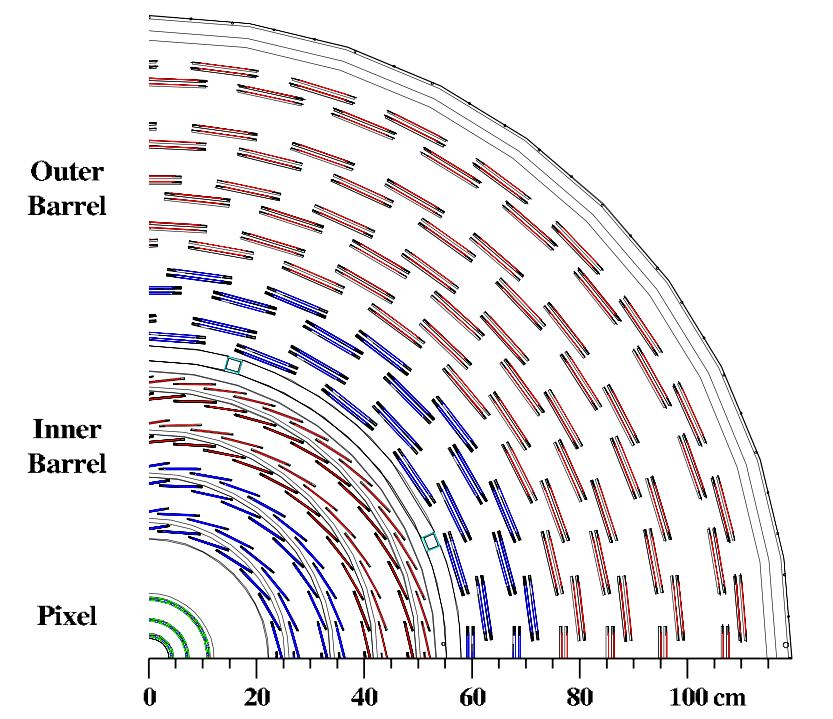
\includegraphics[width=0.6\textwidth]{tracker}
  \caption[A quadrant of the cross section of the barrel part of the {CMS}
tracker.]{A quadrant of the cross section of the barrel part of the {CMS}
tracker. From \cite{cmsgsf}.}
  \label{fig:tracker}
\end{figure}

A quadrant of the cross sections of the barrel part of the {CMS}
tracker is shown in \FigureRef{fig:tracker}.
The tracker utilises silicon pixel detectors in the innermost layers where the
particle flux is the highest.  Outside of the pixel detector, the tracking
detector comprises several layers of silicon microstrip detectors where the
particle flux is smaller.  The total active area of silicon in the CMS tracker
is over \unit{200}{\meter\squared} \cite{chatrchyan2008cms}.

\subsubsection{Pixel Tracker}
The pixel tracker consists of three layers of hybrid silicon pixel detectors in
the barrel region and two in the endcap region. 
The barrel layers are positioned at radii of 4.4, 7.3 and \unit{10.2}{\cm} and have
a length of \unit{53}{\cm}. The two layers in each endcap are located at
$|z|=34.5$ and \unit{46.5}{\cm} with an inner radius of \unit{6}{\cm} and an
outer radius of \unit{15}{\cm}.

\begin{figure}[htbp]
  \centering
  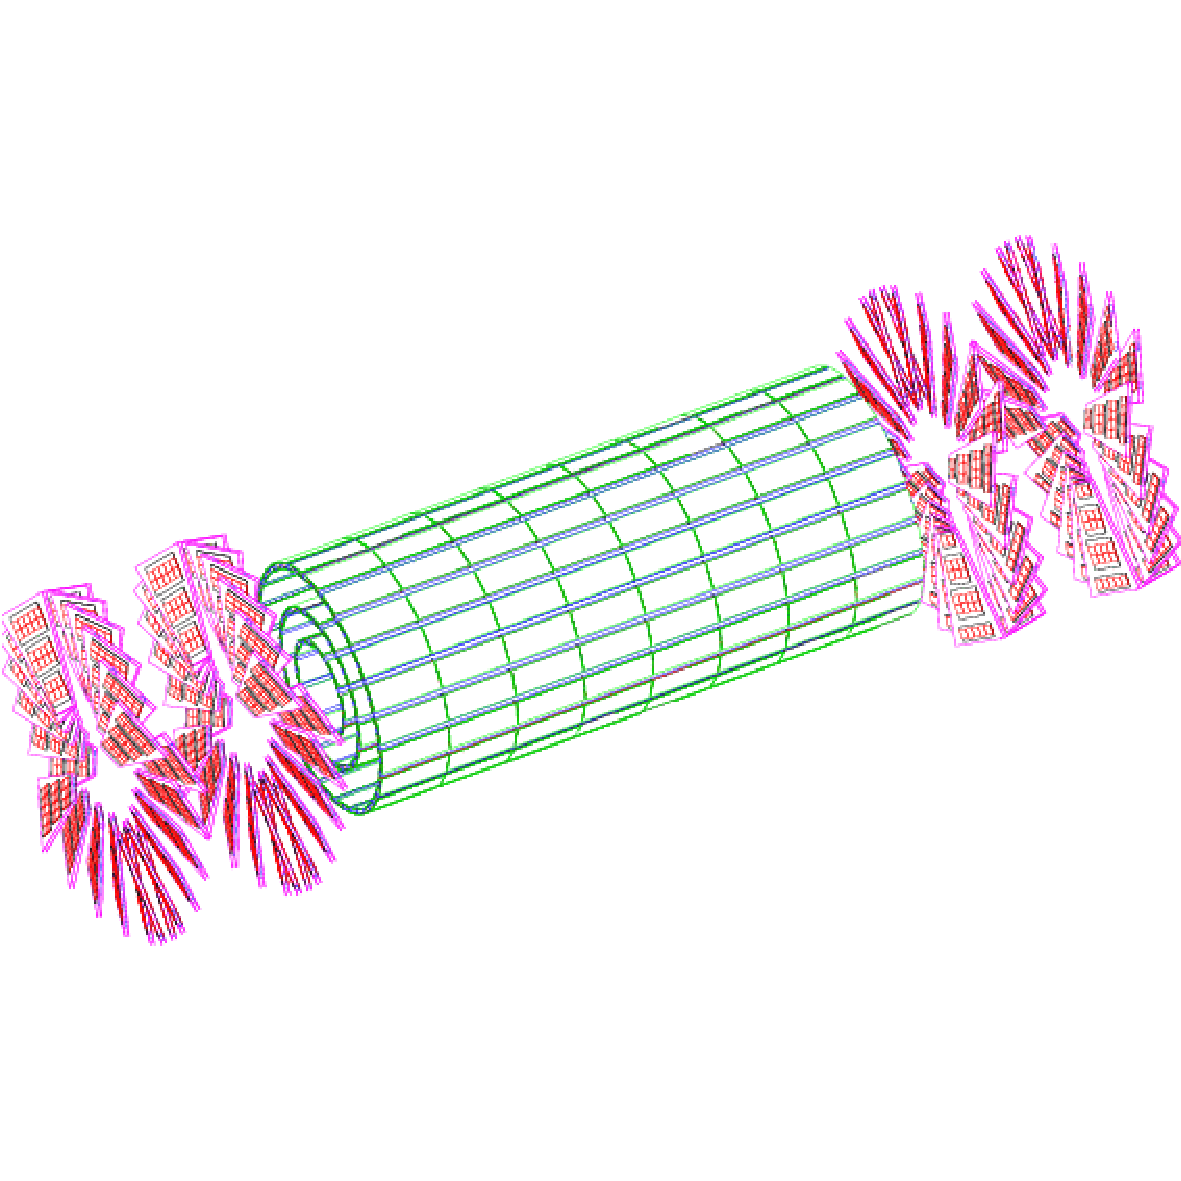
\includegraphics[width=0.75\textwidth]{pixel}
  \caption[The layout of pixel detector in the CMS tracker.]
  {The layout of pixel detector in the CMS tracker. From \cite{chatrchyan2008cms}.}
  \label{fig:pixel}
\end{figure}

A close up view of the pixel tracker is shown in \FigureRef{fig:pixel}.  
Each pixel has a surface area of \unit{$100\times150$}{\micron} which results in
an average particle occupancy of $\mathcal{O}(10^{-4})$ per pixel per crossing.

\subsubsection{Strip Tracker}
The barrel strip tracker comprises two parts, the inner (TIB) and outer (TOB)
trackers.  The TIB is made of 4 layers and covers the longitudinal region $|z|
< \unit{65}{\cm}$ and the region \unit{$20<r<55$}{\cm} in the radial direction.
The TIB utilises microstrip detectors with a cell size of
$\unit{10}{\cm}\times\unit{80}{\micron}$ with an average occupancy of
$\approx\unit{2-3}{\%}$.

The TOB is formed of 6 layers with a half-length of $|z| < \unit{110}{\cm}$. In
this region the flux is low enough to allow for the use of larger pitch
silicon microstrips with a cell size of
$\unit{25}{\cm}\times\unit{180}{\micron}$ with an average occupancy of
$\approx\unit{1}{\%}$.

The endcaps are separated into the Tracker End Cap (TEC) and the Tracker Inner
Disks (TID). The TEC is split into nine disks and covers the region
$\unit{120}{\cm} < |z| < \unit{280}{\cm}$. The TID comprises three rings
and fills the gap between the TEC and the TIB.

%\subsubsection{Performance}

\subsection{Electromagnetic Calorimeter}
The electromagnetic calorimeter (ECAL) is designed to measure the energy of
electrons and photons with a high resolution. It has a fine lateral granularity
to help with shower separation. It is a hermetic, homogeneous calorimeter
comprising 61200 individual lead tungstate ($PbWO_{4}$) scintillation crystals
in the barrel region ($|\eta|<1.479$) closed by 7324 crystals in each of the two
endcap parts ($1.479<|\eta|<3.0$) \cite{ecal1997technical}.

Lead tungstate crystals are ideally suited for this since the scintillation
decay time is similar to the LHC bunch crossing time, 
with $80\%$ of light being produced within \unit{25}{\ns}.
They also have a short radiation length ($X_0=\unit{0.89}{\cm}$) 
and Moliere radius (\unit{2.2}{\cm}) as well as being radiation hard
(up to \unit{10}{\mrad}).

A disadvantage to using lead tungstate is that the light output of the crystals
is relatively low and changes with temperature. This is overcome by using
photodetectors with an intrinsic gain and maintaining a stable temperature
(within \unit{0.1}{\degreecelsius}).

Silicon avalanche photodiodes (APDs) are used to detect the scintillation light
in the barrel and vacuum phototriodes (VPTs) are used in the endcap parts.

The barrel section of the ECAL (EB) surrounds the inner tracker. It comprises 36
identical supermodules that each cover a half length of the barrel
($0<|\eta|<1.479$) and \unit{20}{\degree} in $\phi$. Each supermodule contains 1700
crystals arranged in a $\phi$-$\eta$ grid with each crystal mounted in a
``semi-projective'' geometry, and aligned \unit{3}{\degree} off the nominal
interaction vertex.  The alignments in the longitudinal and transverse planes
are shown in \FigureRef{fig:crystaltilt} and \FigureRef{fig:crystallong}
respectively. The non-pointing geometry prevents particles escaping through the
gaps between the crystals \cite{ecal1997technical}.  Each crystal has a
cross section of \unit{$22 \times 22$}{\mm\squared} and a length of
\unit{230}{\mm} ($\unit{25.8}{X_0}$).

\begin{figure}[p]
  \centering
  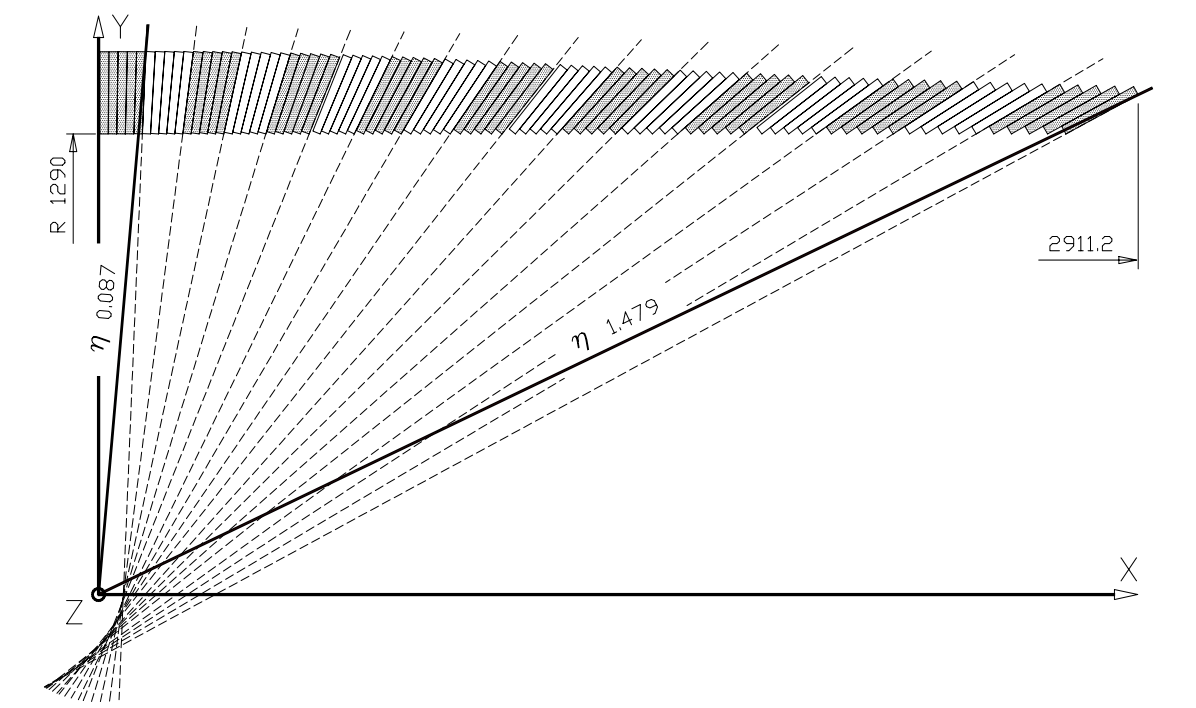
\includegraphics[width=0.7\textwidth]{crystallong}
  \caption[The crystal alignment in the longitudinal view.]{The crystal
alignment in the longitudinal view. The dotted lines show the alignment of the
edge of the crystals. A single supermodule is shown. From \cite{ecal1997technical}.}
  \label{fig:crystallong}
\end{figure}

\begin{figure}[p]
  \centering
  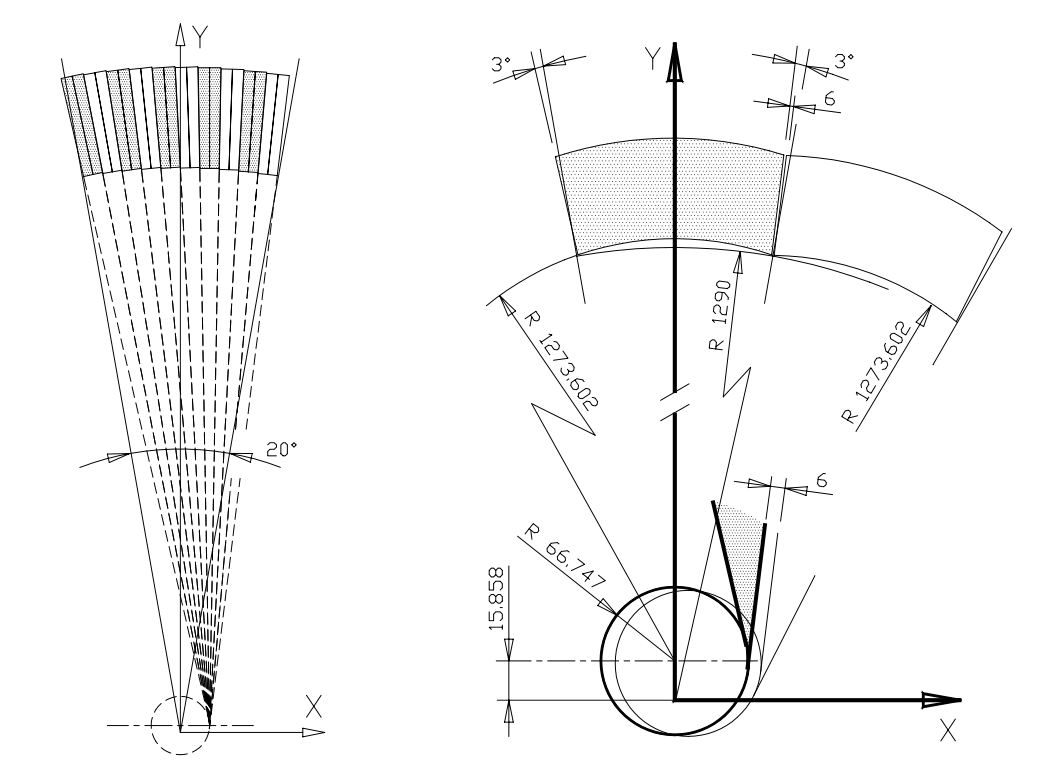
\includegraphics[width=0.7\textwidth]{crystaltilt}
  \caption[The tilt of the ECAL crystals in the transverse plane and the
alignment of the supermodules.] {The tilt of the ECAL crystals in the transverse
plane (left) and the alignment of the supermodules (right). The dotted lines
show the alignment of the crystal edges. From \cite{ecal1997technical}.}
  \label{fig:crystaltilt}
\end{figure}

The endcaps (EE) are formed of two ``Dees'', semi-circular aluminium plates
which support the ``supercrystals'', $5\times5$ arrays of crystals. The crystals are
mounted to point away from the nominal interaction vertex by a small angle in a similar way
to the barrel. 
Unlike the barrel the crystals are arranged in an $x$-$y$ grid.
Installed in front of the endcap ECAL is a preshower system which helps with
the rejection of \Ppizero \cite{chatrchyan2008cms}.

\subsubsection{Performance}

Using a \unit{100}{\GeV} test beam, the energy resolution of the {ECAL} was
found to be\cite{chatrchyan2008cms},
\begin{align}
\left(\frac{\sigma}{E}\right)^{2} 
&= \left(\frac{S}{\sqrt{E}}\right)^{2} + \left(\frac{N}{E}\right)^{2} + C^{2}\\
&=
\left(\frac{\unit{2}{\%}}{\sqrt{E}}\right)^{2} +
\left(\frac{\unit{124}{\MeV}}{E}\right)^{2} + 
\left(\unit{0.26}{\%}\right)^{2}  
\end{align}
where $S$ is the stochastic term, $N$ is the noise term and $C$ is the constant
term. The measured {ECAL} energy resolution is shown in \FigureRef{fig:ECAL}. The
stochastic term is due to the statistical fluctuations in the particles produced
in the electromagnetic shower. The noise term is due to electronic noise and
pile-up. The constant term is due to errors such as non-uniform signal
generation and calibration errors \cite{chatrchyan2008cms}.

\begin{figure}[htbp]
  \centering
  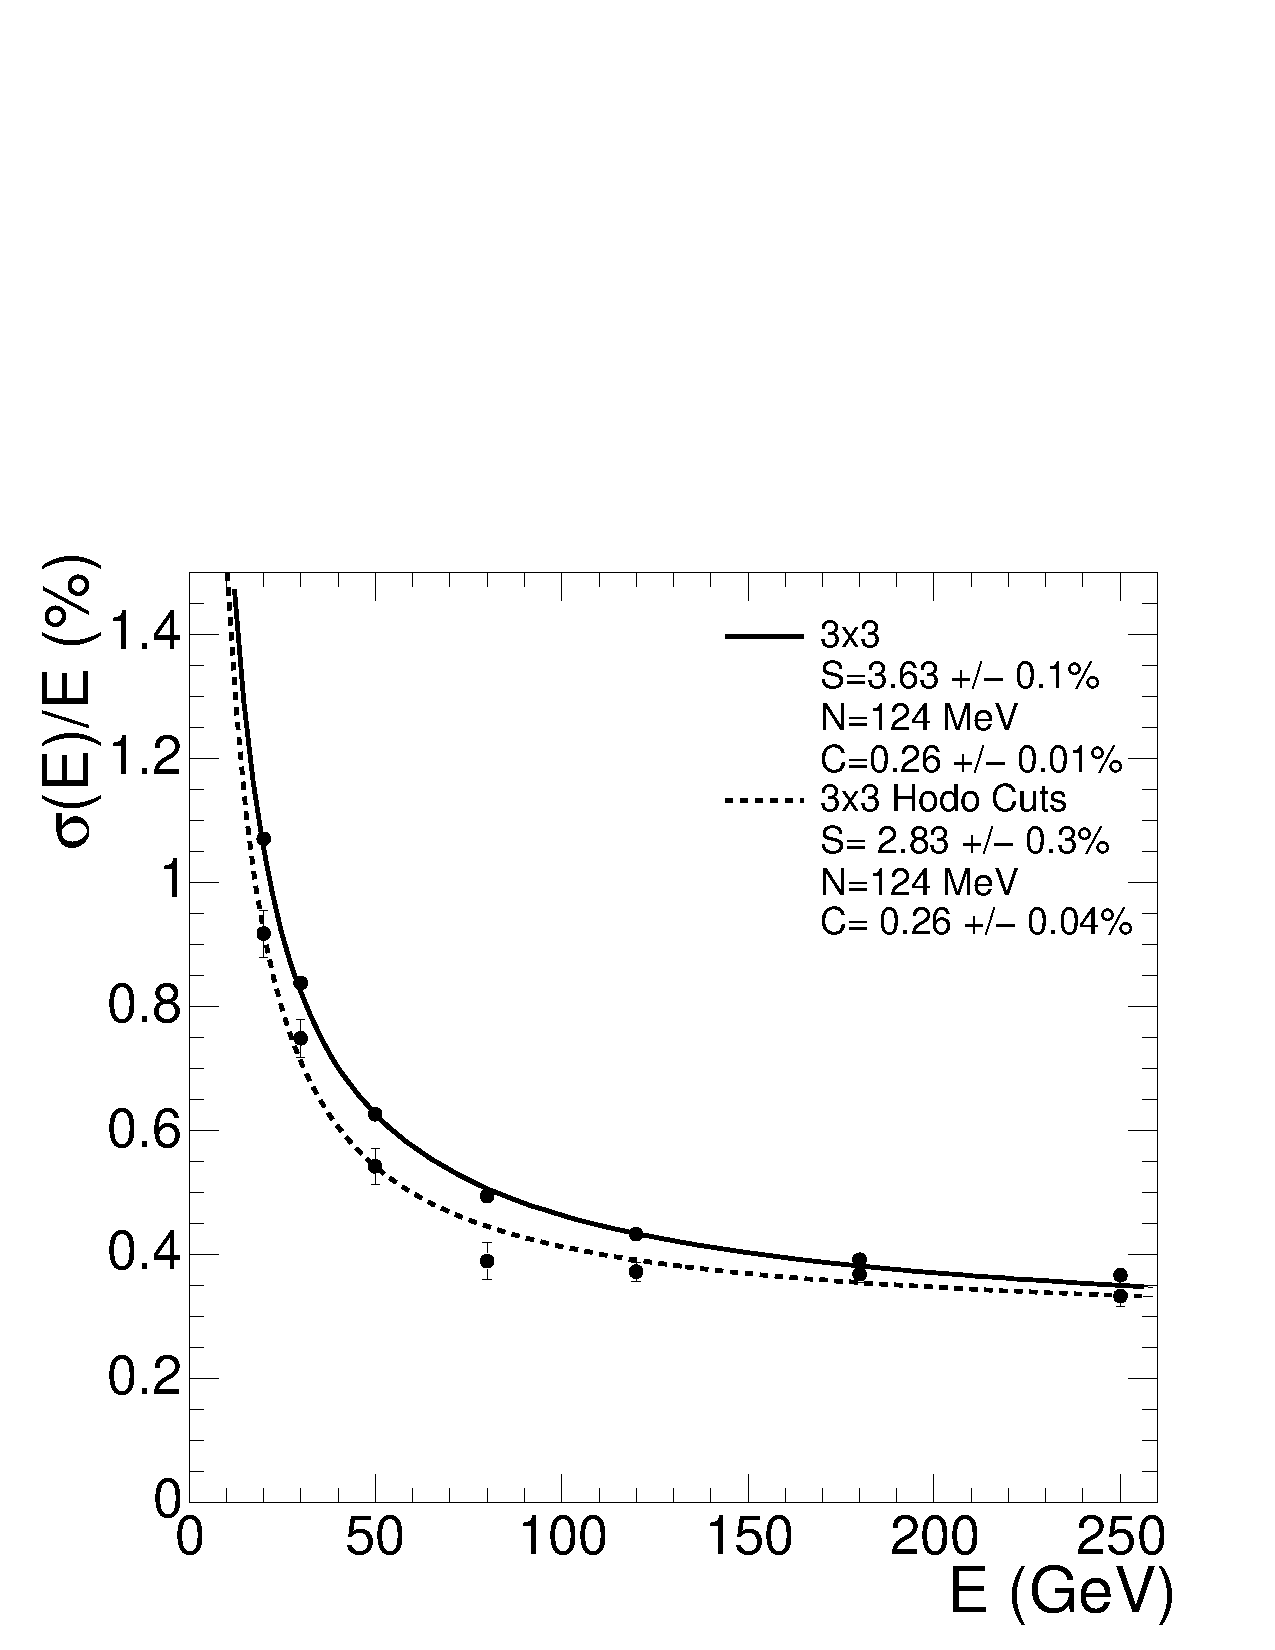
\includegraphics[width=0.7\textwidth]{ecal_performance}
  \caption[Energy resolution $\nicefrac{\sigma}{E}$ of ECAL as a function of
electron energy $E$]{Energy resolution $\nicefrac{\sigma}{E}$ of ECAL as a
function of \label{fig:ECAL} electron energy $E$. From
\cite{chatrchyan2008cms}.}
\end{figure}

\subsection{Hadronic Calorimeter}
The hadronic calorimeter (HCAL), in addition to the electromagnetic calorimeter,
is designed to measure the energy of hadron jets and the missing transverse
energy (\met) which are important signatures in many physics studies at the LHC.

The {HCAL} is a brass/scintillator
sampling hadron calorimeter that covers the region up to $|\eta|<3.0$.  The
scintillation light is channelled by wavelength shifting fibres, that are
embedded in the scintillation tiles, to hybrid photodiodes that can operate in
the high axial magnetic field \cite{chatrchyan2008cms}.

The barrel hadron calorimeter (HB) covers the region ($|\eta| < 1.4$)
and the hadron endcap covers the region $1.4 < |\eta| < 3.0$.

The barrel hadron calorimeter is positioned between the ECAL and the inside of
the solenoid magnet coil ($\unit{1.77}{\meter}<r<\unit{2.95}{\meter}$).  The
strong constraints imposed by the dimensions of the solenoid magnet results in
the HB having an insufficient amount of material to absorb the hadronic shower
in the central region.  To overcome this limitation the outer hadronic
calorimeter (HO) or tail catcher, has been added around the solenoid magnet to
increase the effective thickness of the hadron calorimetry to over 10
interaction lengths.  This provides better protection against punch-through to
the muon system.

\subsubsection{The Forward Calorimeter}
In the forward region ($|\eta| > 3$) energy measurements are made with the
forward hadronic calorimeter, situated \unit{11}{\meter} from the interaction
point. The main role of the forward calorimeter is to improve the \ETm
measurement and to tag jets in the forward direction.

The forward hadronic calorimeter is an iron/quartz-fibre calorimeter where the
Cherenkov light is detected by photomultipliers.  The calorimeter needs to be
radiation hard due to the very large flux in the forward region. However, it is
still expected that after 10 years of operation the light output will be reduced by
about $30\%$ due to the level of radiation \cite{chatrchyan2008cms}. 

\subsubsection{Performance}

\FigureRef{fig:hcalperform} shows the jet energy resolution for three parts of
the {HCAL} measured in test beams. The granularity of the sampling in each
region of the HCAL is such that the resolution is similar in each.

\begin{figure}[htbp]
  \centering
  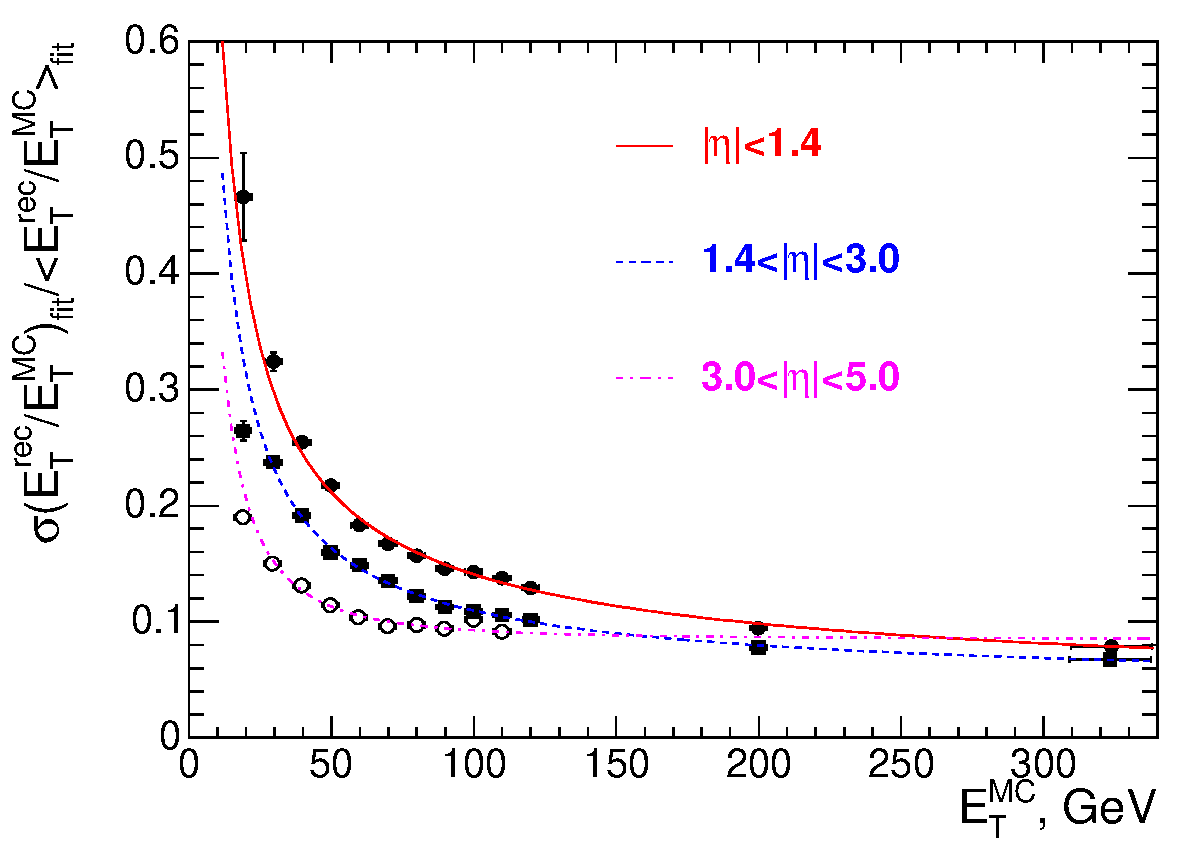
\includegraphics[width=0.7\textwidth]{hcal_performance}
  \caption[The jet transverse energy resolution as a function of jet transverse
energy.] {The jet transverse energy resolution as a function of jet transverse
energy for barrel jets ($|\eta| < 1.4$), endcap jets ($1.4<|\eta| < 3$) and
forward jets ($3<|\eta| < 5$). From \cite{chatrchyan2008cms}. }
  \label{fig:hcalperform}
\end{figure}

\begin{figure}[htbp]
  \centering
  \begin{subfigure}{0.48\textwidth}
    \centering
    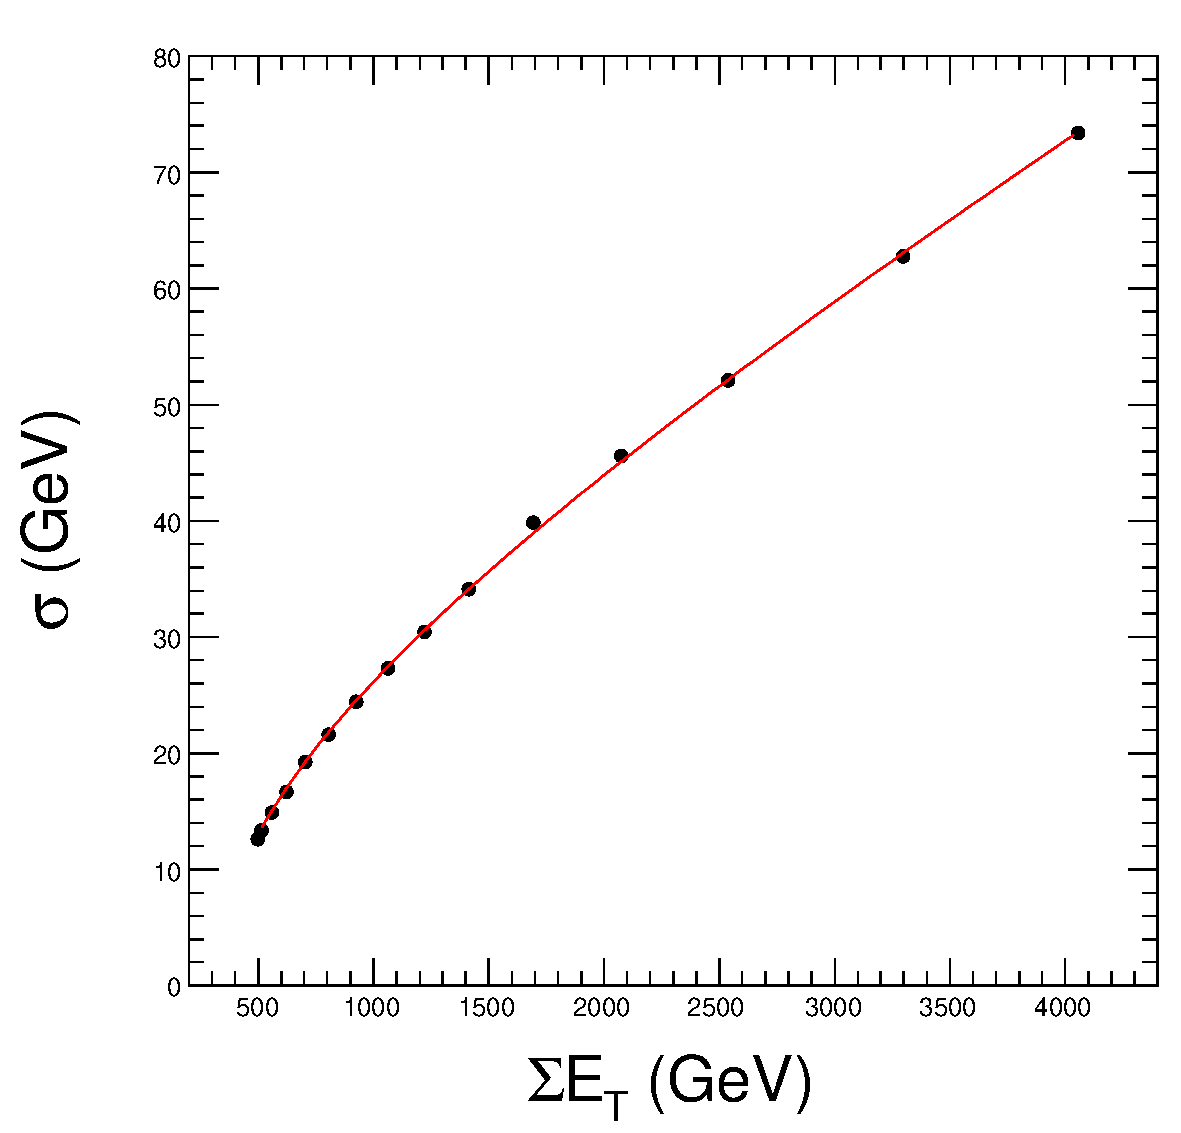
\includegraphics[width=\textwidth]{met_res}
    \caption{\ETm resolution.}
    \label{fig:met_res}
  \end{subfigure}
  \begin{subfigure}{0.48\textwidth}
    \centering
    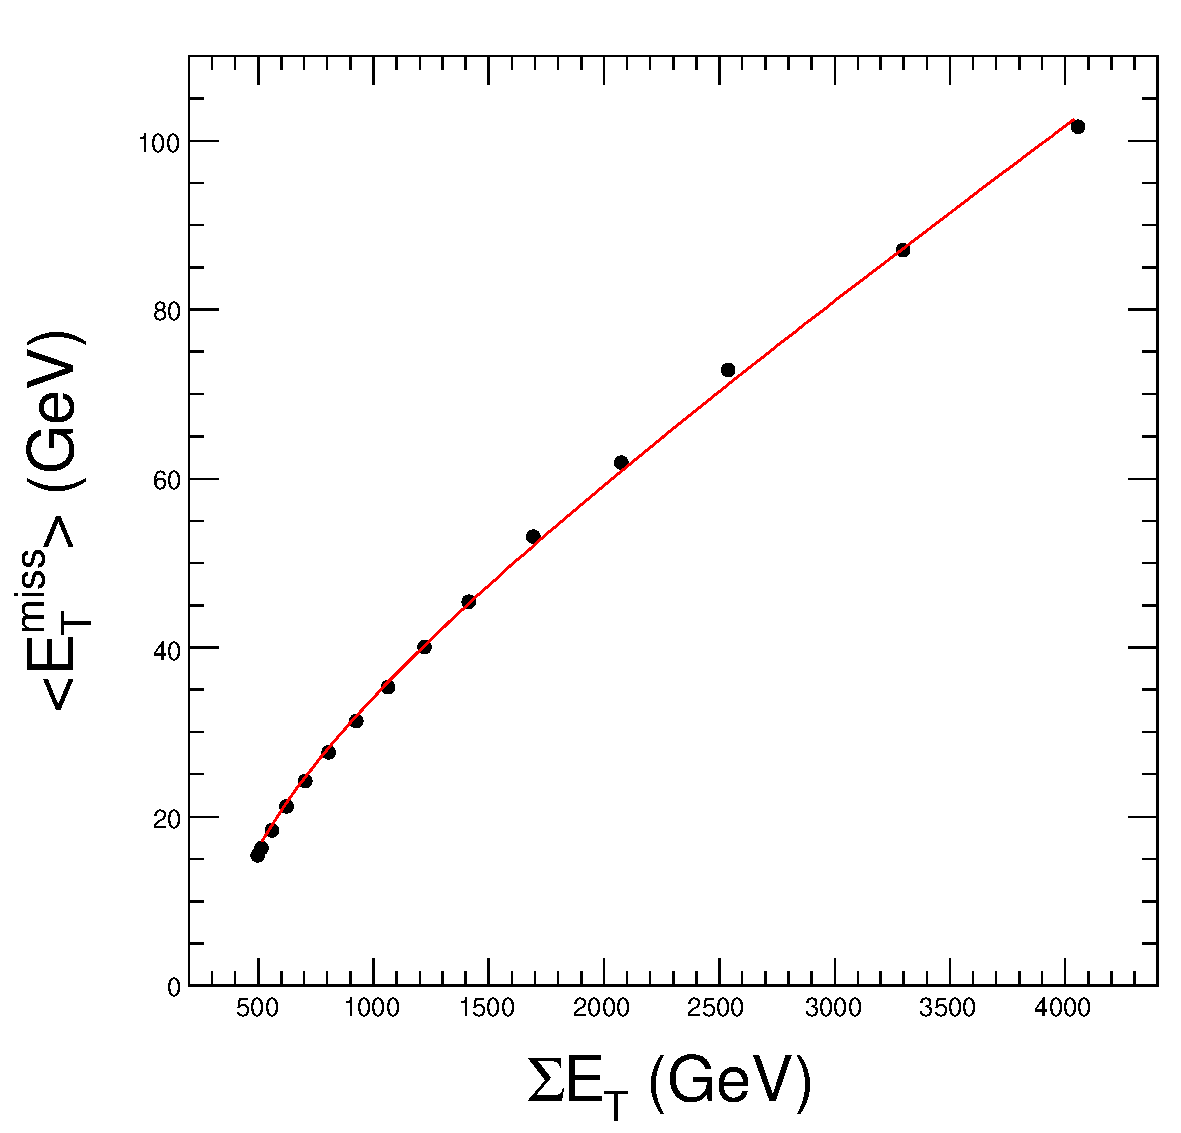
\includegraphics[width=\textwidth]{met_mean}
    \caption{Average reconstructed \ETm.}
    \label{fig:met_mean}
  \end{subfigure}
  \caption[The missing transverse energy performance as a function of the $\sum
E_T$ for QCD events.] { The missing transverse energy performance as a function
of the $\sum E_T$ for QCD events with pile-up. From \cite{chatrchyan2008cms}. }
  \label{fig:met_performance} 
\end{figure}

The performance of the missing transverse energy (\ETm) is shown in
\FigureRef{fig:met_performance} in QCD events. The \ETm resolution is
$\sigma(\ETm) \approx 1.0 \sqrt{\ET}\GeV$ and the average \ETm is
$\langle \ETm \rangle \approx 1.25 \sqrt{\ET}\GeV$
\cite{chatrchyan2008cms}.

\subsection{Muon System}
The muon system lies outside of the CMS solenoid and the outer HCAL detectors.
It is designed to have three functions; to identify muons, measure the momentum
of muons and trigger on muons. To perform these functions the muon system
consists of several different types of detectors due to the different background
rates and magnetic fields in each region of the detector.
The layout of the {CMS} muon system is shown in \FigureRef{fig:muon_system}.

\begin{figure}[htbp]
  \centering
  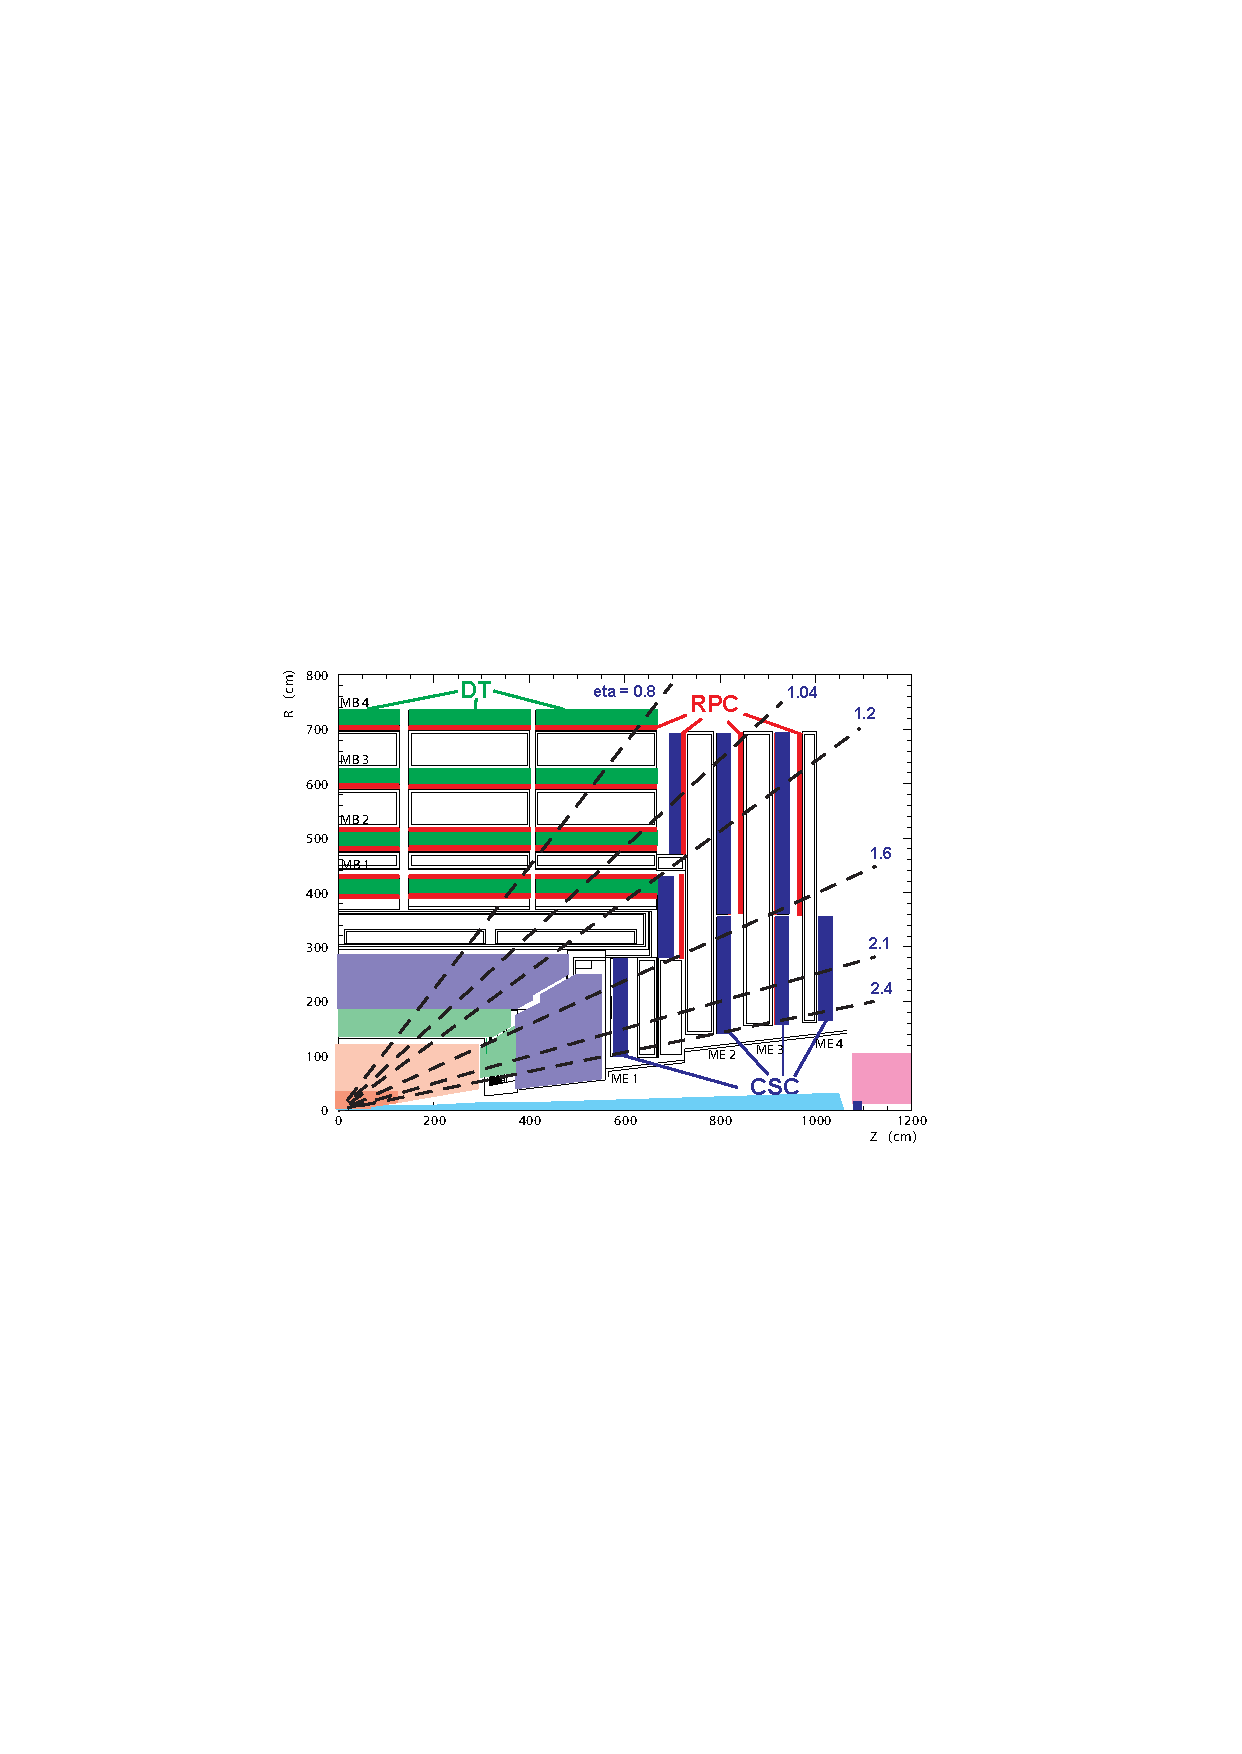
\includegraphics[width=0.8\textwidth]{muon_system}
  \caption[The layout of a quarter of the CMS muon system.] {The layout of a
quarter of the CMS muon system. From \cite{chatrchyan2008cms}.}
  \label{fig:muon_system}
\end{figure}

\subsubsection{Drift Tubes}
In the barrel region ($|\eta| < 1.2$)
where the background rate is low and the residual magnetic field is small,
 aluminium drift tubes (DT) are used,
arranged in four stations interleaved in the flux return
plates. 
Each station contains 12 layers, eight to measure the coordinate in the
$r$-$\phi$ plane and four to measure the $z$ direction (except the fourth station
which only measures the $r$-$\phi$ plane). 

\subsubsection{Cathode Strip Chambers}
In the endcaps ($0.9<|\eta|<2.4$), where the muon and background rate is high and
the magnetic field is also high,
cathode strip chambers (CSC) are used. The
CSCs are arranged in four stations in each endcap. Their faces are perpendicular
to the beam line, and are placed between the flux return plates.  The cathode
strips of each chamber run radially away from the beam line whereas the anode
wires run perpendicular to the strips; both are read out which gives information
on both the $r$-$\phi$ plane (from the cathode) and the $\eta$ direction (from the
anode). \cite{chatrchyan2008cms}

\subsubsection{Resistive Plate Chambers}
In addition to DT chambers and CSCs a complementary trigger system is also used
consisting of resistive plate chambers (RPC) in the endcap and barrel regions.
The RPCs are able to provide a fast and independent trigger over a large range
($|\eta| < 1.6$). In the barrel region, 6 layers of RPCs are used, 2 in each of
the first 2 muon stations and 1 in each of the last 2 stations. In the endcap
there is a layer of RPCs in each of the first 3 stations.

\subsubsection{Alignment}
An optical alignment system, that uses lasers and LEDs, measures the position
of each muon station with respect to each other and the CMS inner tracker to
ensure an accurate and high resolution measurement of the muon
momentum.\cite{chatrchyan2008cms}

\subsubsection{Performance}
The performance of the muon system and inner tracker is shown in 
\FigureRef{fig:muon_performance}. The best resolution for low-momentum muons
is obtained from the measurement in the silicon tracker. However, as the momentum
increases the best resolution is best obtained by combining information
from both the inner tracker and the muon detector.

\begin{figure}[htbp]
  \centering
  \begin{subfigure}{0.48\textwidth}
    \centering
    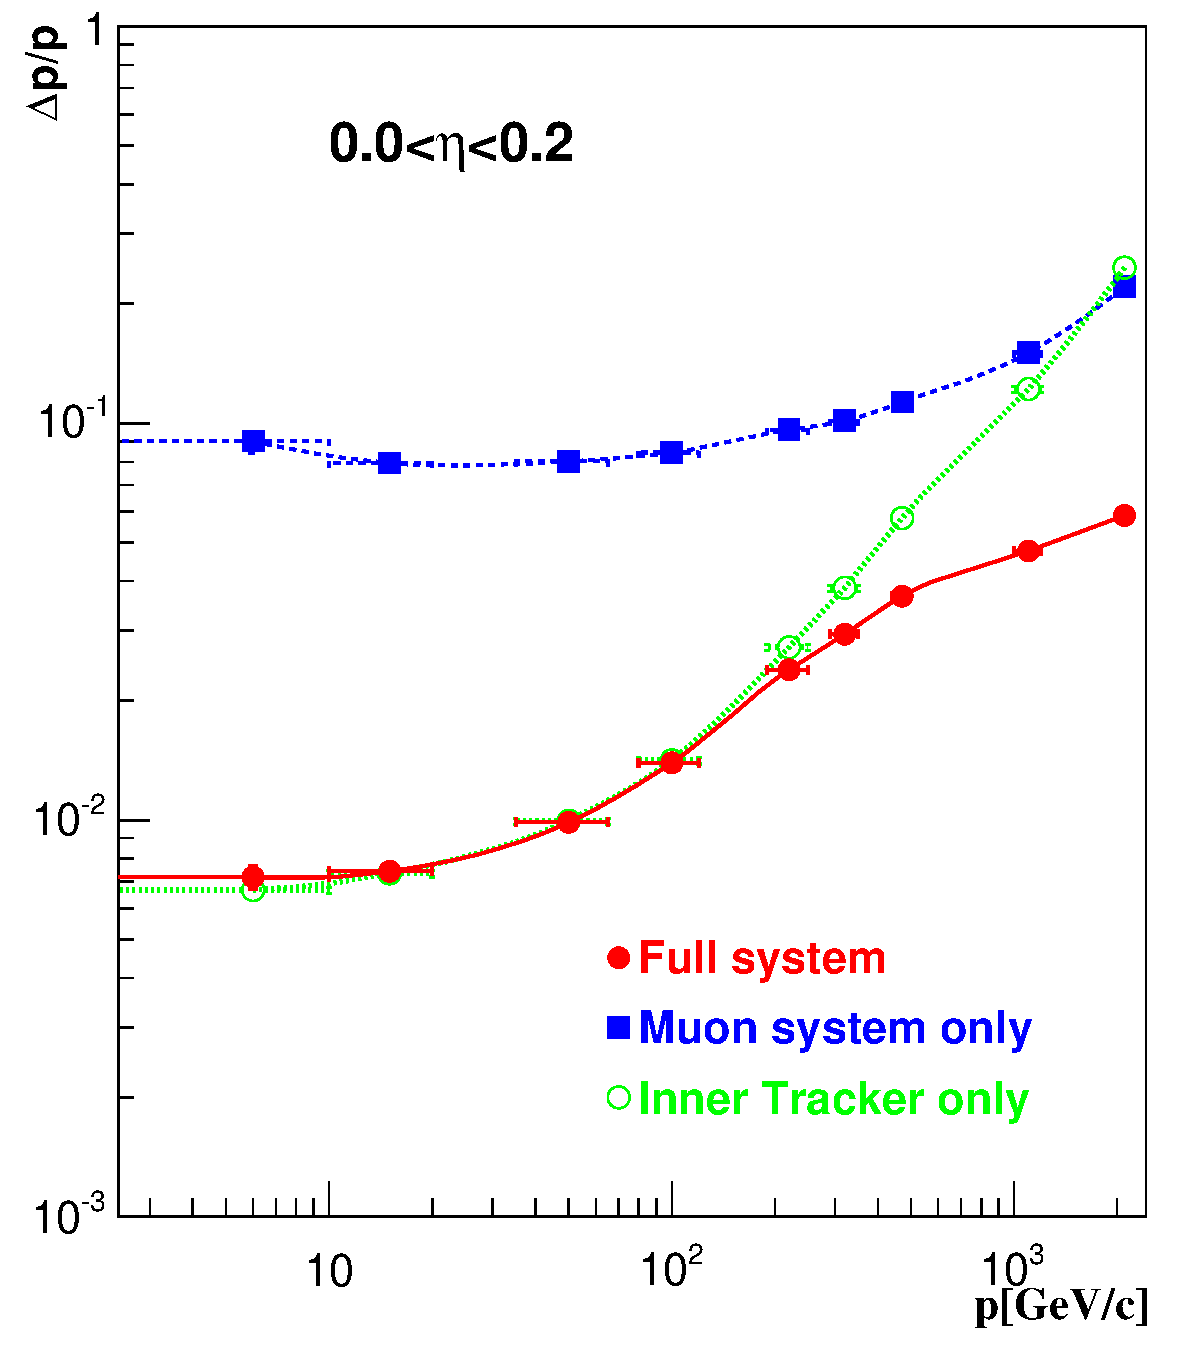
\includegraphics[width=\textwidth]{muon_barrel}
    \caption{Barrel.}
    \label{fig:muon_barrel}
  \end{subfigure}
  \begin{subfigure}{0.48\textwidth}
    \centering
    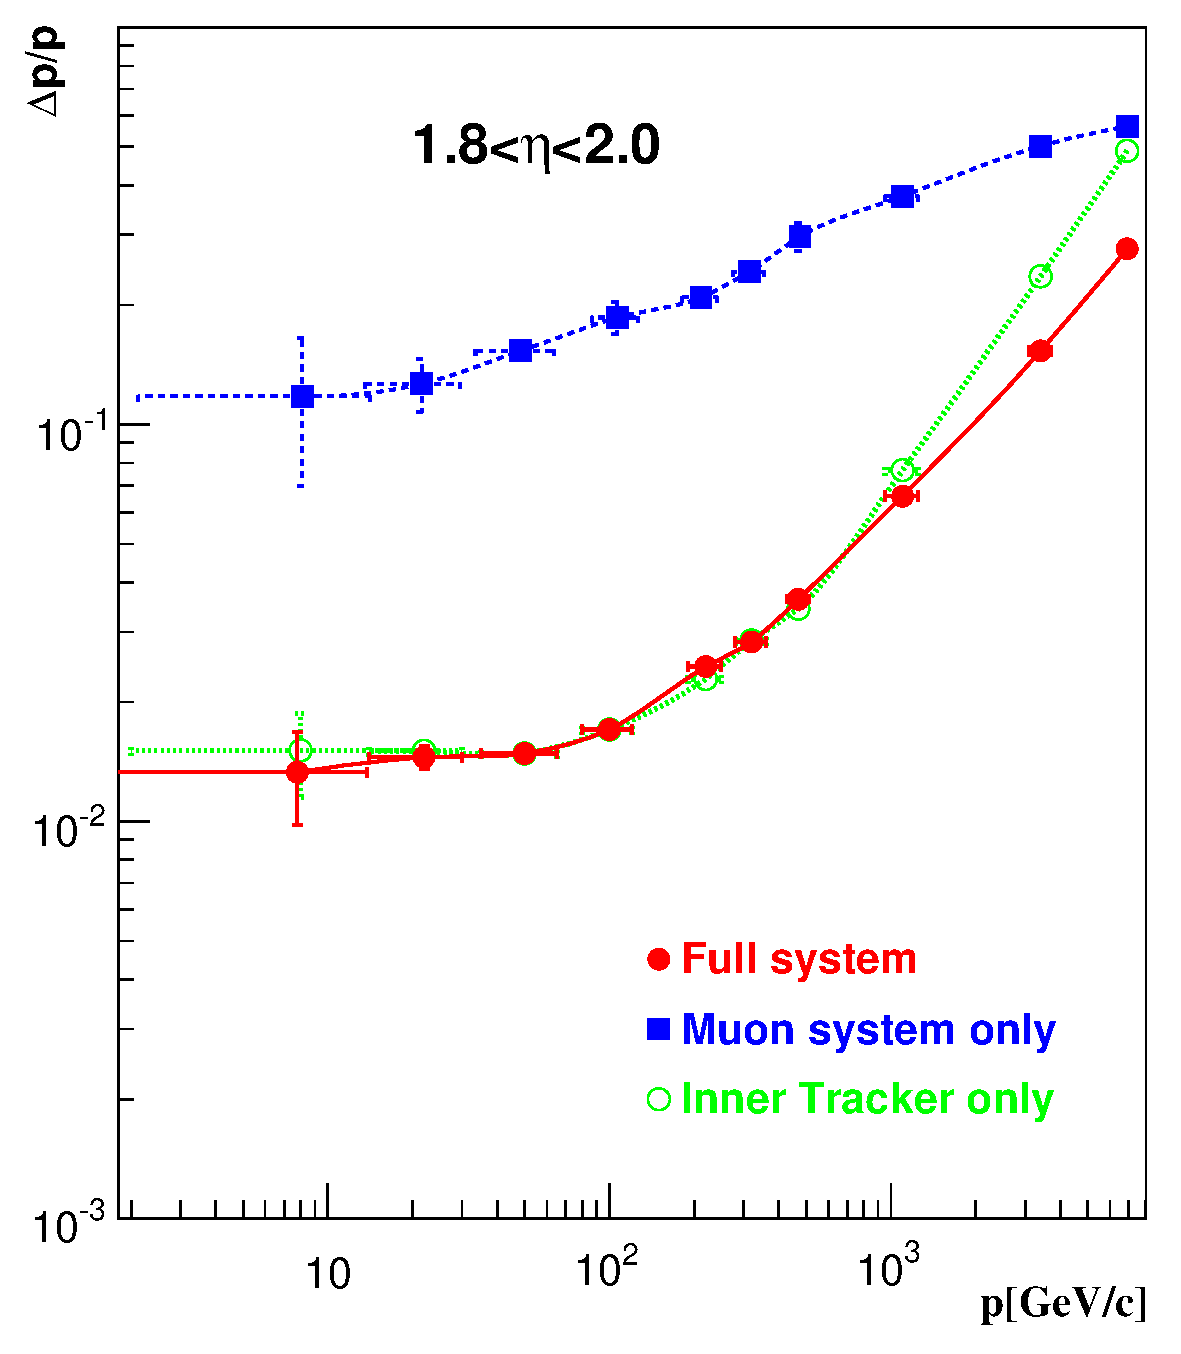
\includegraphics[width=\textwidth]{muon_endcap}
    \caption{Endcap.}
    \label{fig:muon_endcap}
  \end{subfigure}
  \caption[Muon transverse momentum resolution as a function of the muon
momentum.] {Muon transverse momentum resolution as a function of the muon
momentum using only the muon system, only the tracker and both, for barrel muons
($|\eta| < 0.2$) and endcap muons ($1.8<|\eta| < 2.0$). From
\cite{chatrchyan2008cms}.\label{fig:muon_performance}}
\end{figure}

\subsection{Trigger and Data Acquisition}
At design luminosity, the high bunch crossing frequency of the LHC means that
each crossing will contain an average of 20 superimposed inelastic
events every \unit{25}{\nano\second}, a rate of $10^{9}$ interactions per
second.
The size of an event is approximately \unit{1}{\mega\bel} after zero-suppression.
The total data output rate from CMS is $\approx \unit{80}{\tera\bel\per\second}$.
These figures are many orders of magnitude larger than the storage and offline
processing capability available to CMS, which corresponds to about
\unit{250}{\mega\bel\per\second} or about $\approx 10^{2}$ crossings written to the tape
storage every second. 

The vast majority of events will contain only glancing inelastic collisions and
may not be of interest from a physics perspective and can be discarded.  It is
the job of the trigger to reduce the rate of events by a factor of $10^6$ by
rejecting the uninteresting events while keeping as many interesting events as
possible.

An overview of the {DAQ} and trigger is shown in \FigureRef{fig:CMSDAQ}.
The trigger is separated into two parts; the Level-1 trigger and the High
Level Trigger.\cite{chatrchyan2008cms}

\begin{figure}[htbp]
  \centering
  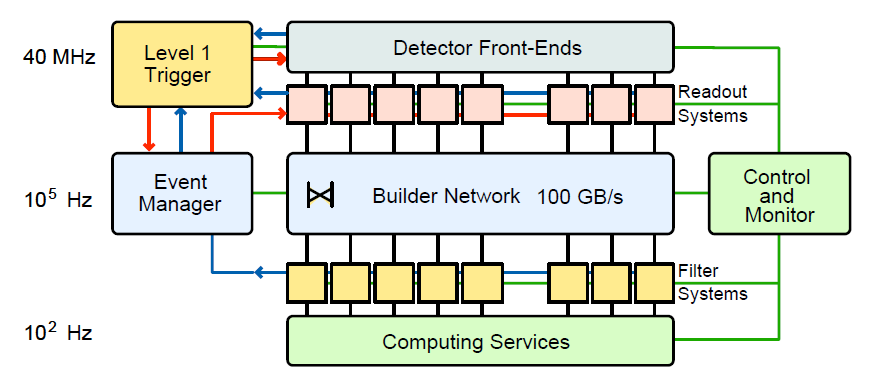
\includegraphics[width=0.85\textwidth]{CMSDAQ}
  \caption[Overview of the architecture of the CMS DAQ and trigger.] {Overview
of the architecture of the CMS DAQ and trigger. From \label{fig:CMSDAQ}
\cite{chatrchyan2008cms}.}
\end{figure}

\subsubsection{Level-1 Trigger}

The Level-1 trigger (L1) is designed to reduce the event rate from the bunch
crossing frequency of \unit{40}{\mega\hertz} to a maximum output rate of
\unit{100}{\kilo\hertz}.  The L1 trigger is implemented with custom-designed
fast programmable electronics that take as input coarse data from the
calorimeters and muon systems; the high resolution data are placed in pipe-lined
memories awaiting a Level-1 decision. The reduced resolution and granularity data are used to form ``trigger
primitives'', such as isolated high energy electromagnetic deposits that pass a
certain \PT or \ET threshold, upon which the L1 Trigger bases its decision. It
also receives information on event-wide variables such as the total sum of
transverse energy and the missing transverse energy.

\subsubsection{High-Level Triggers}
After a fixed time interval of \unit{3.2}{\micro\second} the high resolution
event data held in the pipeline memories are either read out or discarded
depending on the decision at the Level-1 trigger.  The data are transferred to a
processor running the high-level trigger software.

The high-level trigger (HLT) is a software system which runs on a server farm
with over one thousand commercial multicore processors with access to the
complete event data allowing it to make more complex calculations. 
Objects are reconstructed in the HLT as they are needed and events are discarded
as soon as possible to avoid wasting processing time.
The decision to accept an event is based on the requirements on the datasets
used in {CMS} analyses. A typical data-set requires a high \pT
HLT-reconstructed object or an amount of missing transverse energy in the event.
For example, the data-sets relevant to this thesis require a single high \pT
electron, as is described in \SectionRef{sec:trigger1} and
\SectionRef{sec:trigger2}.

\subsubsection{Computing}

The {CMS} data are available in several different file formats that contain
different levels of details \cite{grandi2004cms},
\begin{itemize}
\item Raw data, is the output of the events that pass the {HLT}. The files
contain the detector data, the {L1} trigger results, the {HLT} trigger
results and the higher-level objects that are created during the {HLT}
process.
\item Reconstructed (RECO) data, is the output of the reconstruction process.
The files contain the reconstructed physics objects and reconstructed hits and
clusters.
\item Analysis Object Data (AOD), is the reduced event representation and
contains only the reconstructed objects. This is the format that is used to
perform physics analyses.
\end{itemize}

CMS utilises a distributed computing model called the ``Grid''.  The Grid
consists of several clusters of computers distributed around the world and
organised into several tiers \cite{grandi2004cms}.  Events that pass the {HLT}
are sent to the primary Tier-0 centre where the raw data are stored on tape
before undergoing prompt reconstruction. The reconstructed data are distributed
to Tier-1 and Tier-2 centres at national laboratories and universities around the
world. The roles of the Tier-1 and Tier-2 sites are to run the physics analyses
and to reprocess the data when updated calibrations are available. This is
typically done once or twice a year.


  \chapter{Physics Objects}
\label{chap:objects}

In this chapter the algorithms used to reconstruct analysis objects and
quantities from individual measurements from different parts of the CMS detector
are described.

\begin{figure}[htbp]
  \centering
  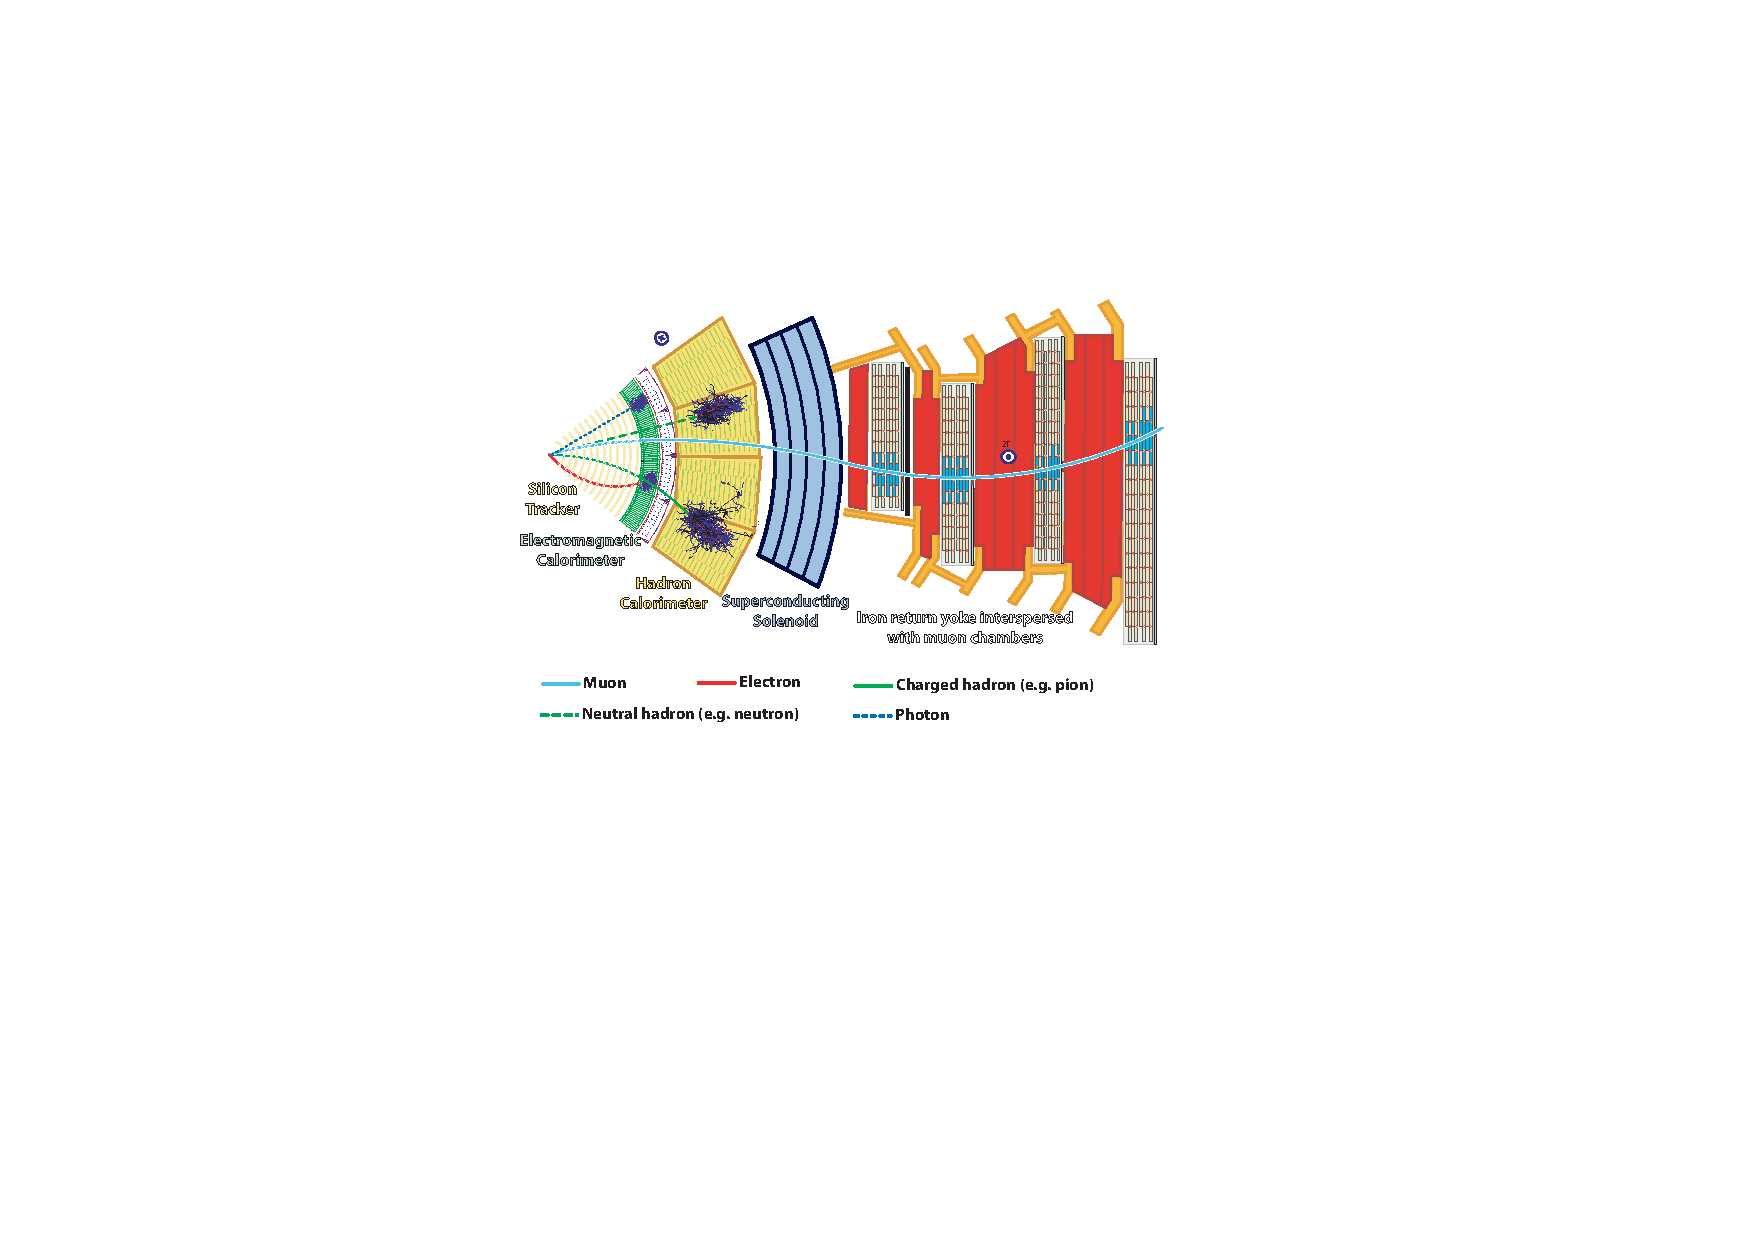
\includegraphics[trim=8cm 8cm 9cm 5cm, width=\textwidth]{slice}
  \caption[The path of different particles through a cross section of the CMS
detector.] {The path of different particles through a cross section of the CMS
detector. From \cite{cmsslice}.}
  \label{reco:crosssec}
\end{figure}

\FigureRef{reco:crosssec} shows a cross section of {CMS} superimposed with the
typical paths of several different particles and their interactions with the
sub-detectors of {CMS}.  This chapter describes how the information
from each sub-detector is combined to identify and reconstruct the particles.

\section{Electrons}
Electrons are important physics objects in CMS as they provide easy-to-identify
signatures and their energy can be measured with a good resolution. This section
will describe the electron reconstruction algorithms used to produce electron
candidates, and the identification variables used to discriminate between real
electron candidates and their backgrounds.

\subsection{Reconstruction}
Electrons are reconstructed in CMS using information from the pixel detector,
silicon strip tracker and the ECAL.  The first step of the reconstruction is to
collect together energy deposits in the ECAL. Next, the path of the electron
though the tracker is reconstructed and matched to the energy deposits in the
ECAL\cite{baffioni2007electron,adam2009electron}.

\subsubsection{Electron Clustering}

In addition to ionisation energy losses and multiple Coulomb scattering,
electrons will suffer large energy losses while traversing the inner detector by
a process called bremsstrahlung.  As electrons interact with the atomic nuclei,
the nuclear electric field accelerates the electron, and the energy change
appears in the form of a photon \cite{perkins2000introduction}.  The photon may
then undergo pair production, in the field of a nucleus, to produce an
electron-positron pair.  As the electron traverses the CMS tracker, the strong
magnetic field causes the path to be curved in the azimuthal, $\phi$, direction,
so that the electron is accompanied by a ``spray'' of electromagnetic energy
that is spread in the ECAL over a narrow strip in the $\phi$ direction. 
\FigureRef{fig:brem} shows the fraction of energy radiated by bremsstrahlung for
electrons of energy 10, 30 and \unit{50}{\GeV} \cite{baffioni2007electron}.

\begin{figure}[htbp]
  \centering
  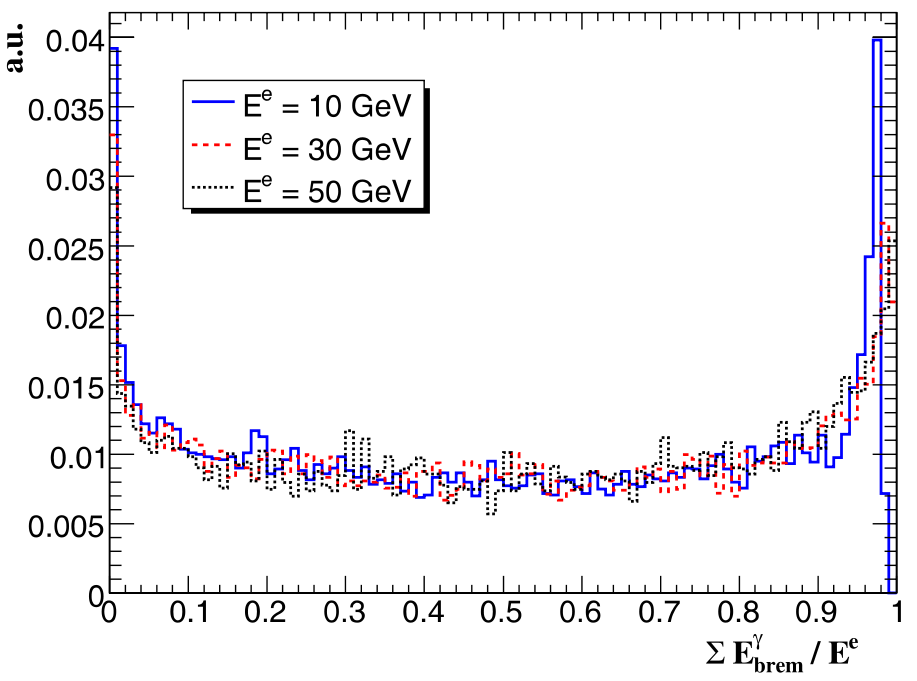
\includegraphics[width=0.7\textwidth]{brem}
  \caption[Distribution of the fraction of electron energy radiated away as
bremsstrahlung photons.] {Distribution of the fraction of electron energy,
$E^{e}$, radiated away as bremsstrahlung photons, $\sum E_{brem}^{\gamma}$. From
\cite{baffioni2007electron}.}
\label{fig:brem}
\end{figure}

To measure the electron energy, the separated deposits of energy need to be
collected together, using ``super-clustering'' algorithms. 
In the barrel a ``hybrid'' algorithm is used. The hybrid algorithm proceeds by
identifying crystals with energies above a certain threshold, that will act as
seeds. The algorithm then forms $5\times1$ or $3\times1$ crystal ``dominos'' in
$\eta\times\phi$, centred on the seed crystal, depending on the
energy within the domino. The dominos are then collected together in the $\phi$
direction, up to an angle of \unit{0.3}{\rad}, to form clusters of dominos,
as demonstrated in \FigureRef{fig:hybrid} \cite{meschi2001electron}

\begin{figure}[htbp]
  \centering
  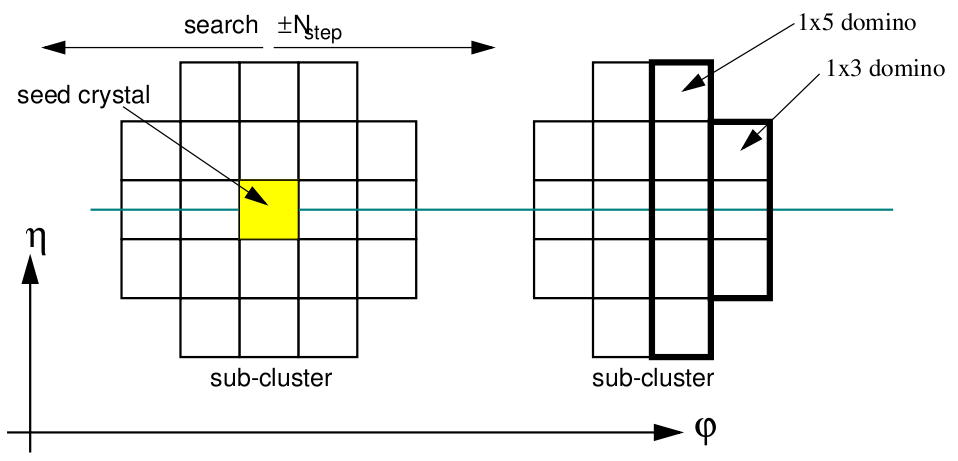
\includegraphics[width=0.85\textwidth]{hybridalgo}
  \caption[Demonstration of the clustering of dominos in the hybrid algorithm.]
{Demonstration of the clustering of dominos in the hybrid algorithm.  From
\cite{meschi2001electron}. The algorithm starts on the seed crystal and clusters
$3\times1$ and $5\times1$ dominos to form the first subcluster. The algorithm
continues to search by stepping in $\phi$ and identifies a second subcluster.}
  \label{fig:hybrid}
\end{figure}

A ``multi5x5'' algorithm is used in the ECAL endcaps. Energy is collected in
$5\times5$ crystal arrays which are then collected together, if their position lies on
a narrow $\phi$ road, to form superclusters \cite{meschi2001electron}.

\subsubsection{Electron Seeding}
The superclusters are then used to select seeds for the track reconstruction.
Starting with a supercluster that passes a \pt threshold,
the trajectory of the electron is propagated back through the magnetic field and
matched to pairs or triplets of hits in the inner tracker that act as trajectory
seeds.  If the trajectory seeds fall within a window of the supercluster path
under either charge hypothesis, they are selected and used to seed the track
reconstruction.  This ECAL-driven seeding is complemented by a tracker-driven
seeding algorithm.  This starts with high purity tracks and extrapolates them
outwards to the ECAL, and is more effective for lower \pt electrons
\cite{baffioni2007electron,adam2009electron}.

Seeds from both of the algorithms are collected and merged into a single
collection, which is then used to seed the electron track reconstruction.

\subsubsection{Electron Track Reconstruction}
The track reconstruction is based on a combinatorial Kalman filter \cite{kalman},
with the electron energy losses described using Bethe-Heitler
modelling \cite{bethe}.
The track reconstruction starts from a trajectory seed, from which a tree of
possible track candidates is built. 

The Kalman filter has two steps, the propagation step and the update step. In
the propagation step, track candidates are extrapolated to the next layer of the
detector, while taking into account energy losses due to bremsstrahlung and
Coulomb scattering.  In the update step, the extrapolated track candidate is
combined with the observed track hit in that layer and the track parameters are
updated. 

The collected hits are passed to the Gaussian Sum Filter (GSF) for a final
fitting and estimation of the track parameters \cite{cmsgsf}. The {GSF}
algorithm is similar to the Kalman filter but energy losses are now described by
a weighted sum of Gaussian distributions \cite{gsf}.
% corrections

\subsection{Backgrounds to Prompt Electrons}
In addition to prompt electrons, the electron candidates from the reconstruction
algorithms will contain background signatures, either fake electrons or unwanted
real electrons produced via some background process.

There are two main processes that may produce signatures in the detector that
may be mistakenly identified as an electron and an additional
two processes that may produce real electrons \cite{nikos}.

\subsubsection{Charged hadrons that shower early in the ECAL}
A charged pion will leave a track, that will appear similar to a non-radiating
electron track.
If the pion were to produce a hadronic shower early in the ECAL
the energy deposits in the ECAL could be wrongly identified as an
electromagnetic shower.
As an example, the charge exchange process,
\begin{align}
\Ppiminus + \Pproton \to &\Ppizero + \Pneutron \nonumber \\
                         &\to \Pphoton\Pphoton
\end{align}
would be almost indistinguishable from an electron shower.
The electron reconstruction algorithm would combine the
track and electromagnetic shower to form an electron candidate\cite{nikos}.

\subsubsection{\HepProcess{\Ppipm \Ppizero} overlap}
A charged pion within a jet will produce a charged track whereas a neutral pion
will quickly decay to a pair of photons. If the electromagnetic clusters from
the \Ppizero are matched to the track from the charged hadron, the electron
reconstruction algorithm may form an electron candidate\cite{nikos}.

\subsubsection{Electrons from hadronic decays}
Heavy flavour quarks may decay semi-leptonically to produce real electrons. These
electrons will tend to be less well isolated than prompt electrons from \PW
decays\cite{nikos}.

\subsubsection{Electrons from conversions}
As stated previously, a neutral pion will quickly decay to a pair of photons. As
the photons traverse the tracker material they may convert to produce a pair of
real electrons\cite{nikos,barge2009conversion}.  \FigureRef{fig:conversion}
shows an example of a prompt electron and a pair of electrons from photon
conversion.  Electrons from photon conversions will appear to have a large
distance of closest approach to the beam spot, $d_0$.  The electrons will also
tend to have missing hits in the inner tracker close to the interaction point.
There may also be a partner track nearby with opposite charge.

\begin{figure}[htbp]
  \centering
  \begin{subfigure}{0.49\textwidth}
    \centering
    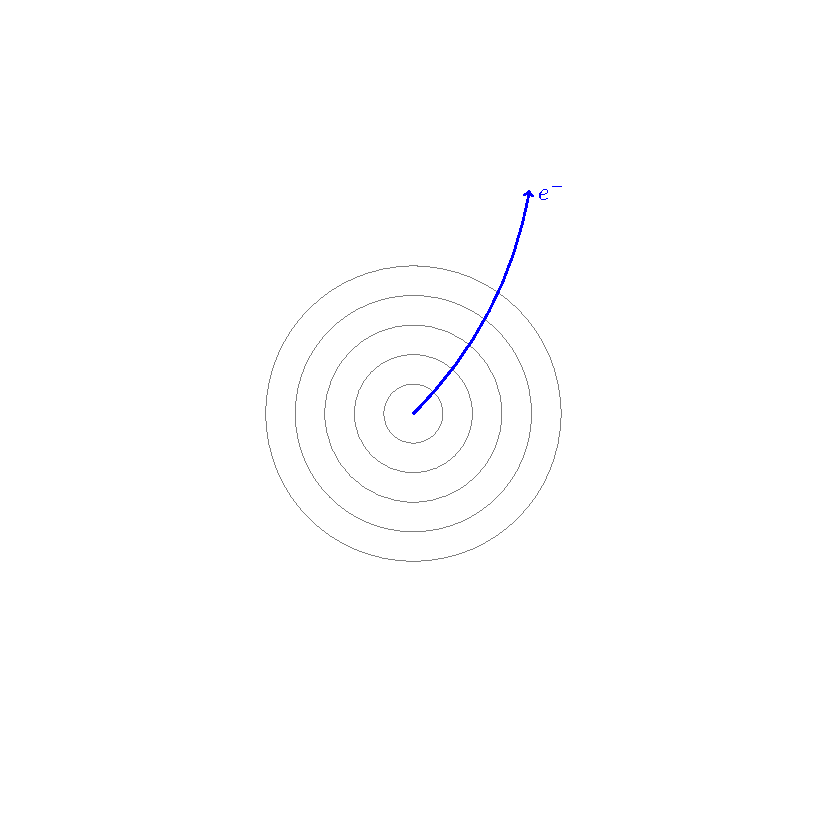
\includegraphics[trim = 35mm 40mm 30mm 30mm, clip,width=\textwidth]{doca_electron}
    \caption{Prompt electron.}
    \label{fig:electron_path}
  \end{subfigure}
  \begin{subfigure}{0.49\textwidth}
    \centering
    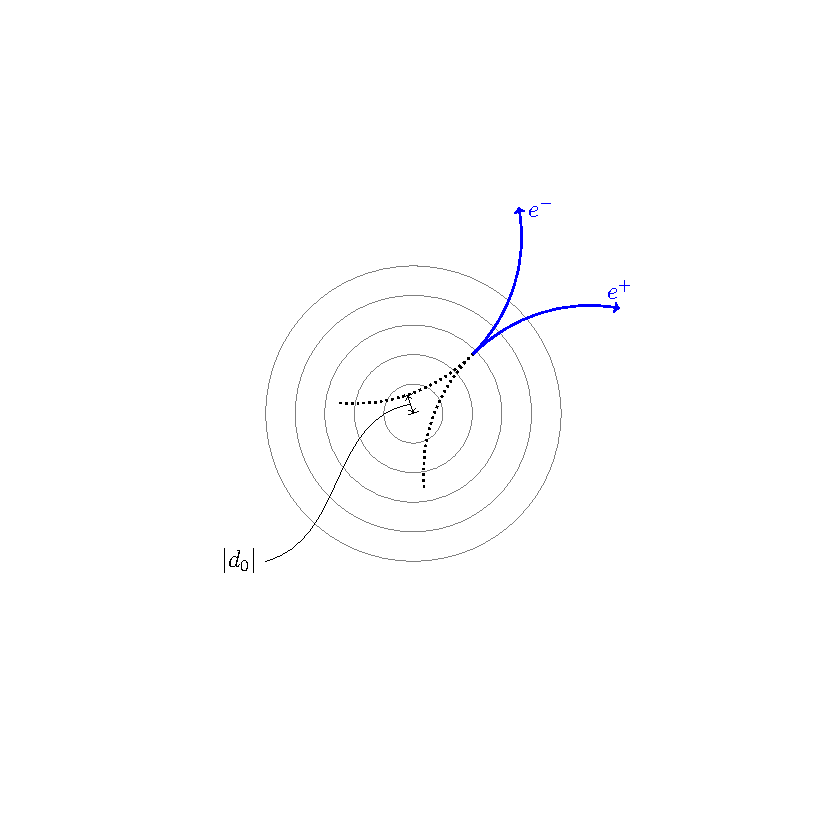
\includegraphics[trim = 35mm 40mm 30mm 30mm, clip,width=\textwidth]{doca}
    \caption{Converted photon.}
    \label{fig:photon_path}
  \end{subfigure}
  \caption[Tracks from an electron and a converted photon in the inner tracker.]
{Tracks from an electron and a converted photon in the inner tracker. Modified
from \cite{barge2009conversion}.}
  \label{fig:conversion}
\end{figure}


\subsection{Electron Identification}
\label{sec:eid}
Electron identification is based on a limited number of variables
\cite{daskalakis2009data,baffioni2009identification}.

\subsubsection{Shape variable}

$\sigma_{\eta\eta}$ is the width of the electron shower in the $\eta$
direction,
\begin{equation}
\sigma_{\eta\eta} = 
\sum_{\text{crystals}} \left(\eta_{i} - \eta_{s}\right)^{2}
\frac{E_{i}}{E_{\text{seed cluster}}}.
\end{equation}
where $\eta_{i}$ and $\eta_{s}$ are the crystal indices in the $\eta$
direction of the $i^{\mathrm{th}}$ crystal and the seed crystal respectively.
$E_i$ is the energy deposited in the $i^{\mathrm{th}}$ crystal.  This variable
discriminates between electrons and jets, as a hadronic shower from a jet or a
pair of photons from a \Ppizero will tend to produce a wider electromagnetic
shower in the $\eta$ direction than a prompt electron.

\subsubsection{Hadronic energy}
The variable $\nicefrac{H}{E}$ is the ratio of the energy deposited in the HCAL
tower behind the electromagnetic seed cluster to the energy of that seed
cluster. This variable offers some discrimination against early showering
hadrons as some of the energy will tend to leak into the HCAL
\cite{baffioni2009identification}.

\subsubsection{Angular separation of track and supercluster}
$\Delta\phi$ and $\Delta\eta$ represent the angular separation between the
trajectory of the reconstructed {GSF} track, extrapolated to the ECAL, and
the ECAL supercluster in the $\phi$ and $\eta$ direction respectively.

\begin{align}
|\Delta\eta| &\equiv |\eta_{\text{SC}} - \eta_{track}|\\
|\Delta\phi| &\equiv |\phi_{\text{SC}} - \phi_{track}|
\end{align}

These variables provide discrimination against accidental matching to the track and
supercluster \cite{baffioni2009identification}. 

%The $\Delta\phi$ variable is symmetric with respect to the charge of the
%electron. If there is a misalignment of the tracker, or some detector effect,
%the cut may introduce an difference in the relative efficiency of electrons
%and positrons. 
%dphi-bar
%dphi-end

\subsubsection{Isolation quantities}
For the calorimeter quantities, the isolation is defined as the sum of energy in
a cone of $\Delta R = 0.3$ centred on the supercluster, where $\Delta R$ is
defined in \EquationRef{eq:dR} and the energy deposits associated with the
electron have been removed, divided by the candidate electron \Pt.

The track isolation is defined as the sum of the \Pt of Kalman filter tracks in
a cone of $\Delta R = 0.3 $ centred on the candidate electron, divided by the
candidate electron \Pt.

Isolation offers very good discrimination between electrons and hadrons, as
hadrons that are mistakenly identified as an electron will tend to be
accompanied by other particles, whereas prompt electrons will usually be well
isolated \cite{baffioni2009identification,nikos}.

\subsubsection{Conversion rejection}
Three further variables are included to reject electrons that are produced from
photon conversions. They are the number of missing hits, $\Delta\cot\theta$ and
$dist$. 

The number of missing hits is simply the number of layers in the inner
tracker where an expected hit from the track reconstruction is not detected by
the detector.

The other two variables are based on conversion partner tracks.
Conversion partner tracks are track candidates that are within a cone of $\Delta
R < 0.3$ around the electron candidate track, and have an opposite charge. 
$\Delta\cot\theta$ is defined as,
\begin{equation}
\Delta \cot \theta \equiv \cot(\theta_{\text{KF}}) - \cot(\theta_{\text{{GSF}}}),
\end{equation}
where $\theta_{KF}$ and $\theta_{{GSF}}$ are the polar angle of the conversion
partner track and the {GSF} track of the electron respectively.
The $dist$ variable is the distance between the two tracks at the point where
they are parallel to one another in the $x-y$ plane as shown in
\FigureRef{fig:dist} \cite{baffioni2009identification,barge2009conversion}.
\begin{figure}[htbp]
  \centering
  \begin{subfigure}{0.45\textwidth}
    \centering
    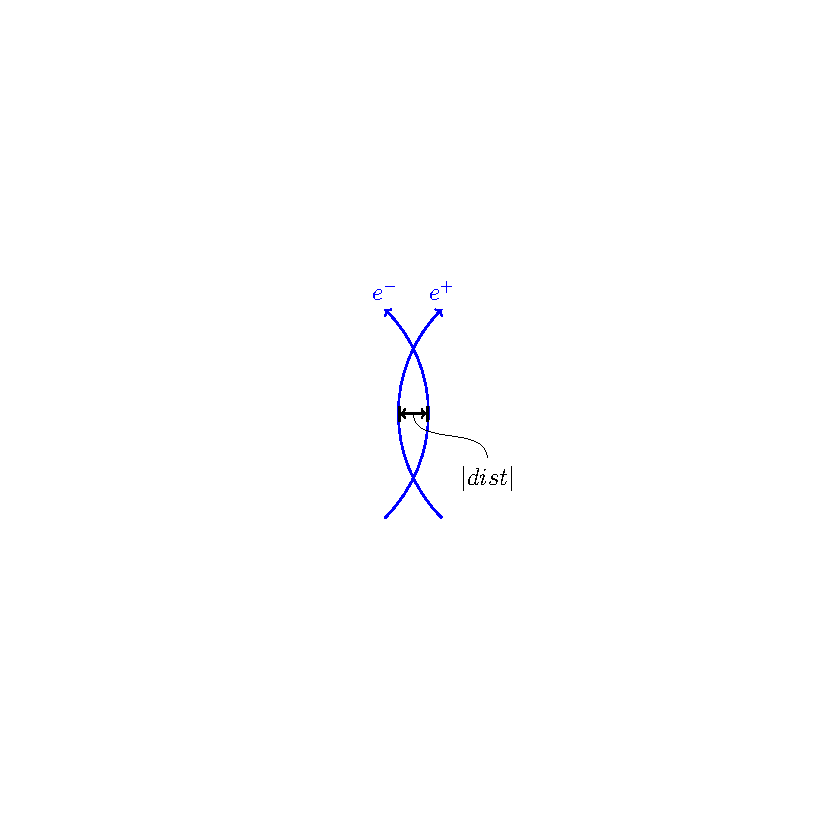
\includegraphics[trim = 40mm 40mm 40mm 40mm, clip,width=\textwidth]{dist_m}
    \caption{$dist<0$.}
    \label{fig:dist_m}
  \end{subfigure}
  \begin{subfigure}{0.45\textwidth}
    \centering
    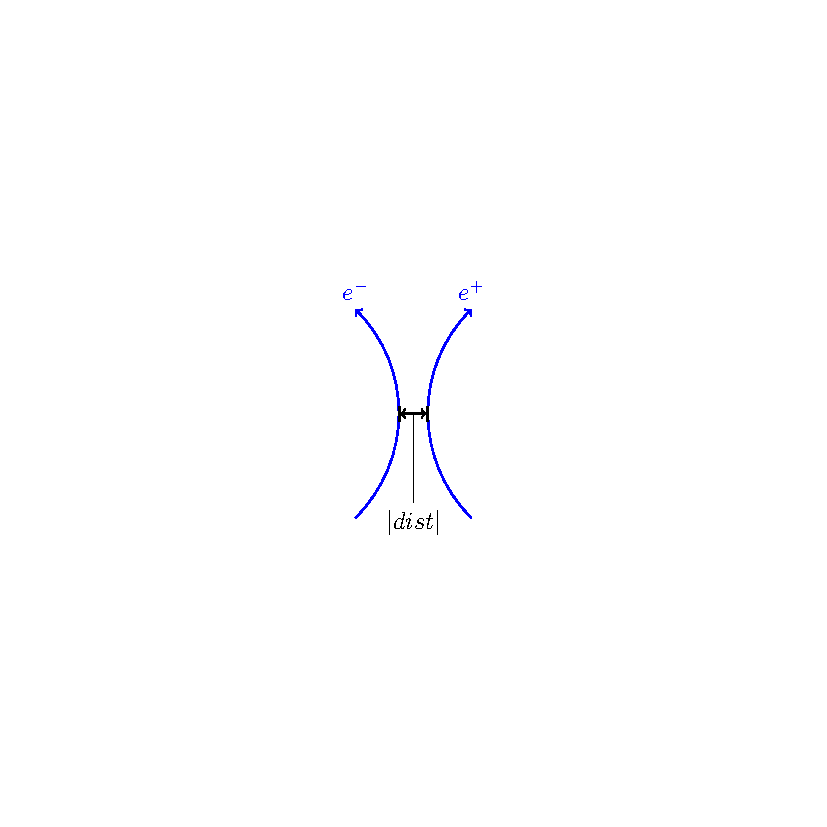
\includegraphics[trim = 40mm 40mm 40mm 40mm, clip,width=\textwidth]{dist_p}
    \caption{$dist>0$.}
    \label{fig:dist_p}
  \end{subfigure}
  \caption[$dist$ is the distance between the two tracks where they are
parallel.]{$dist$ is the distance between the two tracks where they are
parallel. $dist$ is defined to be negative in the case that the tracks overlap
and positive otherwise. Modified from \cite{barge2009conversion}. } 
\label{fig:dist}
\end{figure}

\subsubsection{Electron identification working points}

Several sets of cuts have been produced for CMS analyses. Each set of cuts has
been optimised for a specific efficiency value, or working point
\cite{nikos,daskalakis2009data,simplecutbasedeleid}.  The cut values are
summarised in \TableRef{tab:electronwp}. The cuts can be split into three
categories, ID Cuts, isolation cuts and conversion rejection cuts. Different
sets of cut values are used for electrons in the ECAL barrel and endcap. The cut
values are obtained by simultaneous optimisation for an electron with
$\ET=\unit{25}{\GeV}$. Although the efficiency and background rejection of the
cuts is dependent on the \ET of the electron, the cut values obtained are found
to be effective in the range \unit{15-100}{\GeV} \cite{nikos,daskalakis2009data}.

\begin{table}[htbp]
  \begin{center}
    \begin{tabular}{lllllll} 
\toprule
Efficiencies& $95\%$& $90\%$& $85\%$& $80\%$& $70\%$& $60\%$\\
\midrule
\multicolumn{7}{l}{\emph{Conversion Rejection Cuts}}\\ 
Missing Hits $\leq$& 1& 1& 1& 0& 0& 0\\
$\vert \text{Dist} \vert$ (cm) & N/A& 0.02& 0.02& 0.02& 0.02& 0.02\\
$\vert\Delta\cot\theta\vert$& N/A& 0.02& 0.02& 0.02& 0.02& 0.02\\
\midrule
\multicolumn{7}{l}{Barrel}\\ 
\multicolumn{7}{l}{\emph{Relative Isolation Cuts}} \\
Track    & 0.15& 0.12& 0.09& 0.09& 0.05& 0.04\\
ECAL     & $-$ & 0.09& 0.08& 0.07& 0.06& 0.04\\
HCAL     & 0.12& 0.10& 0.10& 0.10& 0.03& 0.03\\
\multicolumn{7}{l}{\emph{Electron ID Cuts}} \\
$\sigma_{i\eta i\eta}$& 0.01& 0.01& 0.01& 0.01& 0.01& 0.01\\
$\Delta \phi$& $-$ & $-$ & 0.06& 0.06& 0.03& 0.025\\
$\Delta \eta$& 0.007& 0.007& 0.006& 0.004& 0.004& 0.004\\
H/E& 0.15& 0.12& 0.04& 0.04& 0.025& 0.025\\
\midrule
\multicolumn{7}{l}{End Cap}\\ 
\multicolumn{7}{l}{\emph{Relative Isolation Cuts}} \\
Track    & 0.08& 0.05& 0.05& 0.04& 0.025& 0.025\\
ECAL     & 0.06& 0.06& 0.05& 0.05& 0.025& 0.02\\
HCAL     & 0.05& 0.03& 0.025& 0.025& 0.02& 0.02\\
\multicolumn{7}{l}{\emph{Electron ID Cuts}} \\
$\sigma_{i\eta i\eta}$& 0.03& 0.03& 0.03& 0.03& 0.03& 0.03\\
$\Delta \phi$& $-$ & $-$ & 0.04& 0.03& 0.02& 0.02\\
$\Delta \eta$& 0.01& 0.009& 0.007& 0.007& 0.005& 0.005\\
H/E& 0.07& 0.05& 0.025& 0.025& 0.025& 0.025\\
\bottomrule
    \end{tabular}
    \caption[Electron selection variables and corresponding cut values for
several different efficiency working points.] {Electron selection variables and
corresponding cut values for several different efficiency working points
\cite{nikos,daskalakis2009data,simplecutbasedeleid}.\label{tab:electronwp} }
  \end{center}
\end{table}

\subsection{Charge Identification}
\label{sec:charge}
The charge of an electron can be identified by studying how the electron
trajectory is bent in the magnetic field as the electron passes through the
silicon tracker. This can be made difficult by conversion of bremsstrahlung
photons when they are radiated early.

Within CMS, three methods of charge identification have been developed based on
the {GSF} track charge, the general track charge and the supercluster charge
\cite{adam2009electron}. 

The {GSF} track charge is simply the sign of the curvature of the {GSF} fit of
the electron track.  The general track charge is found by matching the {GSF}
track with a general Kalman filter track by asking for shared hits in the pixel
tracker; the charge is the sign of the curvature of the Kalman filter track.
The supercluster charge is obtained by finding the sign of the $\phi$ difference
between the supercluster position and the first hit of the electron track.

At the \PZ peak, an incorrect charge identification rate of \unit{3}{\%}
\cite{adam2009electron} is measured when using the electron trajectory from the
{GSF} fit.  A sample with improved charge identification can be obtained by
using a majority method, that combines the three measurements and assigns the
sign from the two estimates out of three that are in agreement.  A sample with
even greater improved charge identification can be obtained by requiring that
all three methods for assigning charge are in agreement and discarding the event
otherwise \cite{adam2009electron}.

\section{Muons and Taus}
Muons and taus are not used in the analyses presented in
this thesis. Their reconstruction is only briefly described here.  Muons are
reconstructed from information in the muon chambers and the silicon tracker.
Full details of the muon reconstruction are described in reference
\cite{collaboration2010muon}.

Taus may decay leptonically or hadronically. Leptonically decaying taus will
decay to muons or electrons and may be indistinguishable from prompt
leptons. The reconstruction algorithms for taus are described in reference
\cite{collaboration2012tau}.

\section{Missing Energy} 
Neutrinos are weakly interacting neutral particles that escape the
detector without being directly detected by any of the detector components. 
Instead they can be indirectly detected by measuring the total momentum of the
reconstructed particles in an event.
An imbalance in the total momentum of the event can be assigned to undetected
particles. 
This is called the missing energy in the event.

In a hadron collider, the initial longitudinal momentum in the parton
interaction is not
known, so only the kinematic quantities in the transverse place are usually
considered.  One of these is the missing transverse energy, \ETm, and is defined
as the magnitude of the negative vector sum of the momentum of all final state particles in an
event,
\begin{equation}
\vec{E}^{\text{miss}}_{\text{T}} = -\sum_i^{\text{particles}} \vec{p}_{T}^{i},
\end{equation}
where ${E}^{\text{miss}}_{\text{T}} = \vert \vec{E}^{\text{miss}}_{\text{T}}
\vert $.
There are several ways of measuring missing transverse energy.
Calo \ETm is measured by creating pseudo-particles from the energies and
direction of the deposits in the calorimeter towers. The muons are included by
adding their \Pt to the calculation and removing their energy deposited in the
calorimeters. The calo \ETm is then the sum of the transverse energy of the
pseudo-particles.
Track \ETm extends calo \ETm to include the track \Pt in the calculation.  The
corresponding energy deposited in the calorimeters by each track is removed.
Particle flow \ETm (PFMET) is the sum of the transverse energies of all the
reconstructed particle flow particles (see \SectionRef{sec:pf}) \cite{PF}.

\subsection{Particle Flow at CMS}
\label{sec:pf}
The particle-flow event reconstruction attempts to reconstruct and identify all
stable particles in an event by combining information from all CMS
sub-detectors. The particle reconstruction and identification starts with
collecting information from each sub-detector to form elements such as tracks
and energy clusters in the calorimeters. These basic `elements' are then
combined to form blocks which are then interpreted in terms of particles by the
particle flow algorithm. A list of individual particles is then returned from
the algorithm which can be used to study the event in greater detail by,
amongst other things, building jets, tagging b quarks and calculating missing
transverse energy\cite{PF}.

The first step of the particle-flow reconstruction algorithm is to collect the
fundamental elements. The elements consist of charged particle tracks from the
tracker, clusters of energy deposition in the calorimeters and muon tracks.

As a particle traverses the detector it may interact with many CMS sub-detectors
creating several particle-flow elements. A link algorithm is used to connect
the elements together to form blocks that typically contain 1, 2 or 3 elements.
The algorithm returns a distance between the elements as a measure of the
quality of the link. The final step of the particle flow algorithm is to
reconstruct and identify particles from each block of linked elements\cite{PF}.

Once the event has been fully reconstructed with the particle flow technique
the missing transverse energy in the event is computed by
summing up the transverse momentum of all the reconstructed particles\cite{PF}.

\section{Jets}
Jets are reconstructed from information in the tracker and the calorimeters.
Jets are clustered using an anti-$k_t$ algorithm \cite{cacciari2008anti}
with a size of $R=0.5$\cite{collaboration2011determination}.

There are four collections of jets produced by the event reconstruction
algorithms at CMS, Calorimeter (Calo) jets, Particle Flow (PF) Jets, Jet Plus
Tracks (JPT) jets and track jets \cite{collaboration2011determination} . Calo
jets are jets reconstructed from energy deposits in the ECAL and HCAL. JPT jets
extend the Calo jets to include information from the tracker to give an enhanced
\pT resolution. PF jets are produced by the particle flow algorithm\cite{PF}.
Track jets are reconstructed from tracks in the silicon tracker
\cite{collaboration2011determination}.

  \chapter[Measurement of the Electron Charge Asymmetry]{Measurement of the Electron Charge Asymmetry with \unit{36}{\invpb} }
\label{chap:analysis}

In this chapter the measurement of the electron charge asymmetry is presented.
The analysis is performed on the full 2010 dataset, which corresponds to a
luminosity of \unit{36.1}{\invpb} at $\sqrtS = \unit{7}{\TeV}$
\cite{asym36,baisini2010electron}.

The results are presented in 6 bins of absolute value of pseudorapidity with a
fixed width of 0.4. To avoid the gap between the ECAL barrel and the ECAL endcap the
region $1.4<|\eta|<1.6$ is excluded.

\section{Event Selection}

The event selection is performed on single electron datasets formed of events
that are selected using various single photon and single electron triggers. From
these datasets, electrons are selected that pass a limited number of cuts.
Events that contain only a single electron are then selected for the analysis.

\subsection{Trigger}
\label{sec:trigger1}

Several high-level triggers (HLT) were used to select the events due to the
increasing luminosity during the {LHC} 2010 run.  In the initial runs, events
were selected using only a single photon trigger.  As the instantaneous
luminosity was increased and these triggers became prescaled, it was necessary
to use electron triggers to select events.  As the luminosity increased even
further, it was necessary to use electron triggers that included cuts on certain
electron ID variables.

In the following analysis, a control region is obtained by inverting the
selection on the $\Delta\phi$ and $\Delta\eta$ variables (see
\SectionRef{sec:eid}).
To ensure that this inverted selection is effective and will actually
select events, it is necessary to avoid using triggers that apply a selection on
these variables.

The triggers used to select the events are summarised in \TableRef{tab:triggers}
where ``HLT\_Ele$X$'' indicates a high-level trigger selection requiring an
electron with  $\Pt > \unit{X}{\GeV}$.  ``Photon'' in the name indicates that
the selection was applied to ECAL superclusters rather than a reconstructed
electron.  ``SW'' stands for small window, where window refers to the electron
pixel-matching window.  ``Cleaned'' indicates that spikes in the {ECAL} have
been removed.  

``CaloEleId'' and ``TighterCaloIdIso'' represent increasingly tighter selection
based on the shower shape ID and isolation variables from only the {ECAL},
and not the $\Delta\phi$ or $\Delta\eta$ variables.  


``TightEleId'' indicates a tight selection based on all ID variables. 
This nullifies the inverted cuts used for the control region but
it was the only trigger available for these runs without a prescale applied.
To compensate for the missing events in the control region, a looser prescaled
trigger was also applied in these runs.

\begin{table}[htbp]
  \centering
  \begin{tabular}{ l l }
    \toprule
    Run Ranges & Trigger String\\
    \midrule
    132440-137028 & \verb=HLT_Photon10_L1R= \\
    138564-140401 & \verb=HLT_Photon15_Cleaned_L1R= \\
    141956-144114 & \verb=HLT_Ele15_SW_CaloEleId_L1R= \\
    146428-147116 & \verb=HLT_Ele17_SW_CaloEleId_L1R= \\
    147196-148102 & \verb=HLT_Ele17_SW_TightEleId_L1R= \\
                  & \verb=HLT_Ele17_SW_L1R (prescaled)= \\ 
    148822-149063 & \verb=HLT_Ele22_SW_TighterCaloIdIso1_L1R_v1= \\
    149181-149442 & \verb=HLT_Ele22_SW_TighterCaloIdIso1_L1R_v2= \\
    \bottomrule
  \end{tabular}
  \caption{The triggers used to select the data used in this analysis.}
  \label{tab:triggers}
\end{table}

\subsection{Electron Selection}
The available high-level triggers place a lower limit on the electron \pT
threshold.
To avoid a changing HLT efficiency caused by the trigger-turn-on efficiency
curve the electron \PT is required to be
greater than \unit{25}{\GeV} in the analysis. 
The results are presented with an electron \pT cut of 25, 30
and \unit{35}{\GeV}. 

Electron candidates are identified using a cut-based approach on a limited
number of variables \cite{daskalakis2009data}.  The cut values used correspond
to the $80\%$ working point from \TableRef{tab:electronwp}, and are summarised
again in \TableRef{tab:electronselection}. The $80\%$ working point was chosen
as a compromise between ensuring high-enough statistical accuracy while maintaining
a high-enough purity of the sample.

\begin{table}[htbp]
  \begin{center}
    \leavevmode
    \begin{tabular}{lll} 
    \toprule
     Selection Variable & \multicolumn{2}{c}{Cut Value}\\
                        & Barrel & Endcap\\
\midrule 
  \multicolumn{3}{l}{\emph{ID Cuts}}\\
   H/E & 0.04 & 0.025 \\
  $\Delta\phi$ & 0.06 & 0.03 \\
  $\Delta\eta$ & 0.004 & 0.007  \\
  $\sigma_{\eta\eta}$ & 0.01 & 0.03 \\
  \midrule \multicolumn{3}{l}{\emph{Isolation Cuts}}\\
  $ISO_{trk} / E_T $  & 0.09 & 0.04 \\ 
  $ISO_{ecal}/ E_T$  & 0.07 & 0.05 \\
  $ISO_{hcal}/ E_T$  & 0.10 & 0.025 \\ 
  \midrule
   \multicolumn{3}{l}{\emph{Conversion Rejection Cuts}}\\
    Missing Hits  & \multicolumn{2}{c}{$\leq 0$}\\
    Dist (cm) $||$ Dcot   & \multicolumn{2}{c}{$>0.02$}\\
  \bottomrule 
  \end{tabular} 
  \caption[The electron selection variables and corresponding cut values.]
{\label{tab:electronselection}The electron selection variables and corresponding
cut values \cite{simplecutbasedeleid}.} 
  \end{center} 
\end{table}

Incorrectly assigning the charge of an electron will lead to a dilution of the
measured charge asymmetry.  An additional requirement is applied to the charge
of the reconstructed electron to reject events where the true charge is
difficult to determine.  The methods for assigning a charge to an electron are
described in \SectionRef{sec:charge}. The methods are based on the GSF electron
charge, the general track charge and the supercluster charge.
Electron candidates are only selected if all of the three methods agree on the
charge assignment.

The incorrect charge assignment rate can be measured at the Z peak by comparing
the same sign \HepProcess{\PZ\to\Pepm\Pepm} yield to the opposite sign
\HepProcess{\PZ\to\Pelectron\APelectron} yield. \FigureRef{fig:zpeak} show these
Z yields using only the {GSF} track charge (red) and also requiring a unanimous
assignment of charge from all three methods (blue). 

The incorrect charge assignment rate from the GSF track charge alone is about
$3\%$.  By requiring that all three methods for assigning the charge agree, and
vetoing events otherwise, the incorrect assignment rate can be reduced by a
factor of 8 with only a $5\%$ loss in efficiency \cite{baisini2010electron}.

\begin{figure}[htbp]
  \centering
  \begin{subfigure}{\textwidth}
    \centering
    \includegraphics[width=0.75\textwidth]{zpeak_os}
    \caption{Opposite sign \PZ peak.}
    \label{fig:zpeak_os}
  \end{subfigure}
  \begin{subfigure}{\textwidth}
    \centering
    \includegraphics[width=0.75\textwidth]{zpeak_ss}
    \caption{Same sign \PZ peak.}
    \label{fig:zpeak_ss}
  \end{subfigure}
  \caption[$Z\rightarrow ee$ peak.]
{ $Z\rightarrow ee$ peak. One electron is required to be in the
barrel to pass the electron selection and to have a fraction of energy loss by
radiation less than 0.3; the second electron is required only to pass the
electron selection \cite{baisini2010electron}.}\label{fig:zpeak} 
\end{figure}

\subsection{Event Selection}
An event is selected if it contains a single electron that passes all the
electron selection requirements.  To remove Drell-Yan events, an event is vetoed
if it contains a second electron passing a loose selection with $\PT >
\unit{15}{\GeV}$.  Events are also vetoed if they contain an isolated muon with
$\PT > \unit{15}{\GeV}$.

The expected composition of the selected events is measured from the MC
simulation samples, With a \pT cut of \unit{25}{\GeV} it is expected that $65\%$
of selected events are signal events, and of the remaining $35\%$ background
events, the majority are from {QCD} backgrounds with a small number from
{electroweak} processes, which are mostly Drell-Yan (DY) events. 

%\begin{table}[htbp]
%\begin{center}
%\begin{tabular}{llrrr}
    %\toprule
%& & $\PT>25$ \GeV & $\PT>30$ \GeV & $\PT>35$ \GeV  \\
%\midrule
%Signal & \HepProcess{\PW\to\Pe\Pnu} & $65.1\%$&$63.5\%$ &$60.2\%$ \\
%Electroweak & \HepProcess{\PZ\to\Ptau\Ptau} & $0.4\%$ &$0.3\%$  &$0.2\%$ \\
    %& \HepProcess{\PZ\to\Pe\Pe}     & $4.1\%$ &$3.5\%$  &$3.0\%$\\
    %& \HepProcess{\PW\to\Ptau\Pnu}  & $1.9\%$ &$1.1\%$  &$0.6\%$\\
    %& \HepProcess{\Ptop\APtop}      & $0.3\%$ &$0.3\%$  &$0.3\%$\\
    %& Total                         & $6.7\%$ &$5.2\%$  &$4.1\%$\\
%QCD & Total                         & $28.2\%$&$31.3\%$ &$35.7\%$\\
    %\bottomrule
%\end{tabular}
%\caption[Composition of selected events.]{Composition of selected events for lepton momentum cut of
%$\PT>\unit{25}{\GeV}$, $\PT>\unit{30}{\GeV}$ and $\PT>\unit{35}{\GeV}$ from
%{MC} simulation\cite{baisini2010electron}.}
%\label{tab:selectedcomp}
%\end{center}
%\end{table}

The particle flow \ETm distribution for the events that pass the event
selection, with an electron cut of $\PT > \unit{25}{\GeV}$ and $|\eta| < 2.4$ is
shown in \FigureRef{fig:pfmet_dist_36}. There are two obvious peaks in the
distribution. The peak at $\ETm \approx \unit{40}{\GeV}$ is the
\HepProcess{\PW\to\Pe\Pnue} signal region. This region also contains
\HepProcess{\PW\to\Ptau\Pnut} backgrounds. The peak at
$\ETm\approx \unit{10}{\GeV}$ is the background region that contains the {QCD}
and {DY} background events.

\begin{figure}[htbp]
  \begin{center}
    \includegraphics*[width=0.8\textwidth]{pfmet_dist}
    \caption[Particle Flow \ETm distribution for selected events.]{Particle Flow
\ETm distribution for selected events with an electron cut of $\PT >
\unit{25}{\GeV}$ and $|\eta| < 2.4$\cite{baisini2010electron}.\label{fig:pfmet_dist_36}}
  \end{center}
\end{figure}

The number of selected events that pass the
event selection are shown in \TableRef{tab:selectedevents}. To obtain a
measurement of the asymmetry from the selected events it is necessary to extract
the signal yield from each pseudorapidity/charge bin.

\begin{table}[htbp]
\begin{center}
%\begin{sideways}
\begin{tabular}{lcrrr}
    \toprule
  $|\eta|$ range & Charge & \multicolumn{3}{c}{Selected Events}\\
                 &        & $\PT>25$ \GeV & $\PT>30$ \GeV & $\PT>35$ \GeV\\
\midrule
$0.0<| \eta |<0.4$ &$+$& 18956&14232&9885\\
                   &$-$& 15060&11505&8105\\
$0.4<| \eta |<0.8$ &$+$& 20118&14966&10345\\
                   &$-$& 15736&11780&8307\\
$0.8<| \eta |<1.2$ &$+$& 20681&15091&10184\\
                   &$-$& 16167&11735&8112\\
$1.2<| \eta |<1.4$ &$+$& 10646&7606&5161\\
                   &$-$& 8226&5871&4067\\
$1.6<| \eta |<2.0$ &$+$& 16426&11877&7814\\
                   &$-$& 11678&8578&5886\\
$2.0<| \eta |<2.4$ &$+$& 18885&13239&8726\\
                   &$-$& 13226&9227&6184\\
    \bottomrule
\end{tabular}
%\end{sideways}
\end{center}
\caption[Number of events passing the event selection.]{Number of events passing
the event selection for lepton momentum cuts of $\PT> \unit{25}{\GeV}$, $\PT>
\unit{30}{\GeV}$ and $\PT>\unit{35}{\GeV}$ \cite{baisini2010electron}.}
    \label{tab:selectedevents}
\end{table}


\section{Signal Yield Extraction Method}
The number of signal and background events in each bin is extracted using a
maximum likelihood fit to the \ETm distribution using two fixed templates shapes
\cite{adam2007towards}, similar to the method used in the measurement of the \PW
cross section \cite{alcaraz2010updated}.
The first template is the sum of the \Wenu signal and the {electroweak}
background shapes, and the second template is the sum of the {QCD} plus \gjet
processes.

\subsection{{QCD} \ETm Shape}
The \ETm distribution for the {QCD} and \gjet background is obtained from a control.
The control sample is selected by requiring that the electrons pass the
isolation and $H/E$ cuts but fail the $\Delta\phi$ and $\Delta\eta$ cuts as
shown in \TableRef{tab:antisel}.

\begin{figure}[htbp]
  \centering
  \begin{subfigure}{0.4\textwidth}
    \centering
    \includegraphics*[trim = 0mm 0mm 15mm 0mm, clip, width=\textwidth, angle=90]{MetCompare_anti_eta1.pdf}
    \caption{$0.0<| \eta |<0.4$}
    \label{fig:qcd_met_eta1}
  \end{subfigure}
  \begin{subfigure}{0.4\textwidth}
    \centering
    \includegraphics*[trim = 0mm 0mm 15mm 0mm, clip, width=\textwidth, angle=90]{MetCompare_anti_eta2.pdf}
    \caption{$0.4<| \eta |<0.8$}
    \label{fig:qcd_met_eta2}
  \end{subfigure}
  \begin{subfigure}{0.4\textwidth}
    \centering
    \includegraphics*[trim = 0mm 0mm 15mm 0mm, clip, width=\textwidth, angle=90]{MetCompare_anti_eta3.pdf}
    \caption{$0.8<| \eta |<1.2$}
    \label{fig:qcd_met_eta3}
  \end{subfigure}
  \begin{subfigure}{0.4\textwidth}
    \centering
    \includegraphics*[trim = 0mm 0mm 15mm 0mm, clip, width=\textwidth, angle=90]{MetCompare_anti_eta4.pdf}
    \caption{$1.2<| \eta |<1.4$}
    \label{fig:qcd_met_eta4}
  \end{subfigure}
  \begin{subfigure}{0.4\textwidth}
    \centering
    \includegraphics*[trim = 0mm 0mm 15mm 0mm, clip, width=\textwidth, angle=90]{MetCompare_anti_eta5.pdf}
    \caption{$1.6<| \eta |<2.0$}
    \label{fig:qcd_met_eta5}
  \end{subfigure}
  \begin{subfigure}{0.4\textwidth}
    \centering
    \includegraphics*[trim = 0mm 0mm 15mm 0mm, clip, width=\textwidth, angle=90]{MetCompare_anti_eta6.pdf}
    \caption{$2.0<| \eta |<2.4$}
    \label{fig:qcd_met_eta6}
  \end{subfigure}
  \caption[The \ETm distribution in anti-selected {MC}
simulated events and selected {QCD} and \gjet background MC simulated events.]
{The \ETm distribution in data and background anti-selected {MC} simulated
events and selected {QCD} and \gjet background MC simulated events in each
pseudorapidity bin\cite{baisini2010electron}.}
  \label{tab:antiselclosure}
\end{figure}

\begin{table}[htbp]
  \begin{center}
    \leavevmode
    \begin{tabular}{lcc} 
    \toprule
      Selection Variable & \multicolumn{2}{c}{Cut Value}\\
                         & Barrel & Endcap\\
    \midrule
        H/E & 0.04 & 0.025 \\
        $\Delta\phi$ & $>0.06$  & $>0.04$ \\
        $\Delta\eta$ & $>0.007$ & $>0.009$\\
        $ISO_{trk} / E_T $ & 0.09 & 0.04 \\
        $ISO_{ecal}/ E_T$  & 0.07 & 0.05 \\
        $ISO_{hcal}/ E_T$  & 0.10 & 0.025\\ 
    \bottomrule
    \end{tabular}
    \caption[Electron anti-selection variables and corresponding cut values.]
{\label{tab:antisel} Electron anti-selection variables and corresponding cut
values. The $\Delta\phi$ and $\Delta\eta$ cuts are
inverted\cite{baisini2010electron}.}
  \end{center}
\end{table}

To validate the anti-selection used, {QCD} Monte Carlo (MC) simulation samples are used. The
distribution of {QCD} MC events passing the event selection is compared to the
anti-selected MC events. This is shown for each pseudorapidity bin in
\FigureRef{tab:antiselclosure}. The agreement is seen to be good with little
signal contamination in the control region.

\subsection{Signal \ETm Shape from Boson Recoil}
\label{sec:recoil}
The \ETm in signal events arises from the unmeasured neutrino in the event. 
The signal \ETm shape is derived from MC simulations with an event-by-event
correction applied to account for differences in the \ETm scale and resolution
between data and MC.
The correction is based on the hadronic recoil distribution measured in data.
The recoil response and resolution in \HepProcess{\PZ\to\Plepton\Plepton} data
events is measured as a function of the \pT of the boson. This is combined with
information from the \PW and \PZ MC simulation to derive a correction to
the simulated \ETm as a function of \PW boson's \pT
\cite{bauer2010modeling,alcaraz2010updated}.

The transverse recoil vector, $\vec{U}$, is calculated from the reconstructed
transverse missing energy, $\vec{E}_{\mathrm{T}}^{\mathrm{miss}}$, and the
electron \pT vectors,
\begin{align}
\vec{U} &= - \vec{E}_{\mathrm{T}}^{\mathrm{miss}} 
      - \vec{p}^{\ \mathrm{e}}_{\mathrm{T}}\\
\vec{U} &= - \vec{E}_{\mathrm{T}}^{\mathrm{miss}} 
      - \sum_i \vec{p}^{\ \mathrm{e}_i}_{\mathrm{T}}
\end{align}
for \PW events and \PZ events respectively. $\vec{U}$ is split into components
that are parallel ($U_1$) and perpendicular ($U_2$) to the true boson \pT
direction. 
In \PZ data events the true boson \pT is not known and is reconstructed from the
\pT of the two electrons.

The hadronic activity that balances the \pT of the boson will lie mostly in the
$U_1$ direction whereas $U_2$ will be mostly formed from other sources.
\FigureRef{fig:recoil} shows the decomposition of $\vec{U}$ into $U_1$ and
$U_2$ in W events \cite{bauer2010modeling}.
\begin{figure}
  \begin{center}
    \includegraphics*[width=0.85\textwidth]{recoil}
    \caption[The decomposition of $\vec{U}$ for \PW events.] {The decomposition
of $\vec{U}$ for \PW events. Modified from \cite{bauer2010modeling}.}
    \label{fig:recoil}
  \end{center}
\end{figure}

$U_1$ and $U_2$ are measured in \PZ data, \PZ MC simulation and \PW MC
simulation and are then binned in units of the boson \pT.  In each $p_T^{Z}$ bin
the $U_1$ and $U_2$ distributions are fitted with a Gaussian.  A linear function,
$f_i(p_T^Z)$, is fit to the distribution of the Gaussian means to produce a
response curve for both data and MC.  A second order polynomial,
$\sigma_i(p_T^Z)$, is then fit to the distribution of the Gaussian widths to
produce a resolution curve for both data and MC\cite{bauer2010modeling}.

The fitting procedure results in two response functions, $f_i(p_T)$, and two
resolution functions, $\sigma_i(p_T)$, for \PZ data, \PZ MC events and
the \PW MC events. The functions are then used to define a set of \PW
MC corrected functions, 

\begin{align}
f^{corr}_i (p^{W}_T)      
  &= \frac{ f^{Z\ data}_i (p^{Z}_T) }
          { f^{Z\ MC}_i (p^{Z}_T) }
          f^{W\ MC}_i (p^{W}_T) \\
\sigma^{corr}_i (p^{W}_T) 
  &= \frac{ \sigma^{Z\ data}_i (p^{Z}_T) }
          { \sigma^{Z\ MC}_i (p^{Z}_T) }
          \sigma^{W\ MC}_i (p^{W}_T) 
\end{align}

The corrected recoil response and resolution curves are then used to correct the
\PW MC \ETm. For each \PW MC event, the generator level \pT of the boson is
found, and the values for the response, $f^{corr}_i (p^{W}_T)$, and
resolution curves, $\sigma^{corr}_i (p^{W}_T) $, are looked up. A Gaussian is
defined with these values and then sampled to determine the new recoil
components $U_i$,
\begin{equation}
U_i \sim Gaus(f^{corr}_i (p^{W}_T), \sigma^{corr}_i (p^{W}_T) ).
\end{equation}
The components are then combined to form the new corrected recoil vector
$\vec{U^{\prime}}$ which is then combined with the electron vector to
form the corrected \ETm\cite{bauer2010modeling}.

The modelling of the \HepProcess{\PW\to\Plepton\Pnu} \ETm with boson recoil is
described in detail in reference \cite{bauer2010modeling}. 
Ntuples containing \HepProcess{\PW\to\Pelectron\Pnu} simulation with the recoil corrected \ETm were
provided from reference \cite{alcaraz2010updated}.

\subsection{{Electroweak} \ETm Shape}
The electroweak background processes that can produce a single isolated
electron which are considered in this analysis are:
\begin{itemize}
\item \HepProcess{\PZ\to\Pelectron\APelectron}, where one of the electrons falls
outside the geometric acceptance or is not detected,
\item \HepProcess{\PZ\to\Ptauon\APtauon}, where one of the taus decays
to an electron and the other decays hadronically, or semi-leptonically and the lepton
is not detected,
\item \HepProcess{\PW\to\Ptau\Pnu}, where the tau decays to an electron,
\item \HepProcess{\Ptop\APtop}, where an electron is produced.
\end{itemize}

The \ETm distributions for the {electroweak} background were obtained from
PYTHIA\cite{pythia} MC simulations for each pseudorapidity/charge bin.  The MC samples used
are summarised in \TableRef{tab:samples36}.  The scale of the {electroweak}
shape is fixed to the signal \ETm shape by the ratio obtained from MC samples.

\subsection{Fit Results}

The results of the extended maximum likelihood fits to each pseudorapidity/charge
bin are shown the appendix in \FigureRef{fig:fit1} and \FigureRef{fig:fit2} and
the $\chi^2$ of each fit is included in \TableRef{tab:chi2}.
%The signal yield in each bin is summarised in \TableRef{tab:sigyield} and 
%The ratio between the fits and the data for each of the 
%bins are shown in \FigureRef{fig:fit1ratio} and \FigureRef{fig:fit2ratio}.


%\begin{table}[htbp]
%\begin{center}
%\begin{tabular}{lcrrr}
    %\toprule
%$|\eta|$ range & Charge & \multicolumn{3}{c}{Signal Yield}\\
               %&        & $\PT>25$ \GeV & $\PT>30$ \GeV & $\PT>35$ \GeV  \\
%\midrule
%$0.0<| \eta |<0.4$ &$+$& 12866&  9992&  6955\\
                   %&$-$&  9432&  7646&  5476\\
%$0.4<| \eta |<0.8$ &$+$& 13413&  9596&  6898\\
                   %&$-$&  9627&  7128&  5376\\
%$0.8<| \eta |<1.2$ &$+$& 12684&  9161&  5947\\
                   %&$-$&  9013&  6803&  4560\\
%$1.2<| \eta |<1.4$ &$+$&  6220&  4427&  2895\\
                   %&$-$&  4349&  3247&  2231\\
%$1.6<| \eta |<2.0$ &$+$&  9033&  6285&  4079\\
                   %&$-$&  5850&  4270&  2905\\
%$2.0<| \eta |<2.4$ &$+$&  9104&  6965&  4259\\
                   %&$-$&  5420&  4335&  2775\\
    %\bottomrule
%\end{tabular}
%\end{center}
%\caption[The signal yield in each pseudorapidity bin after the fitting
%procedure.]{The signal yield in each pseudorapidity bin after the fitting
%procedure\cite{baisini2010electron}.}
    %\label{tab:sigyield}
%\end{table}

\begin{table}[htbp]
\begin{center}
\begin{tabular}{lcr}
    \toprule
$|\eta|$ range &Charge & $\chi^2$/ndof of Fit\\
\midrule
$0.0<| \eta |<0.4$ &$+$&  0.86\\
                   &$-$&  0.84\\
$0.4<| \eta |<0.8$ &$+$&  0.99\\
                   &$-$&  1.36\\
$0.8<| \eta |<1.2$ &$+$&  1.05\\
                   &$-$&  1.13\\
$1.2<| \eta |<1.4$ &$+$&  0.97\\
                   &$-$&  1.30\\
$1.6<| \eta |<2.0$ &$+$&  1.38\\
                   &$-$&  1.61\\
$2.0<| \eta |<2.4$ &$+$&  1.44\\
                   &$-$&  1.11\\
    \bottomrule
\end{tabular}
\caption[$\chi^2$/ndof of the fits in each pseudorapidity
bin.]{\label{tab:chi2}$\chi^2$/ndof of the fits in each pseudorapidity
bin\cite{baisini2010electron}.}
\end{center}
\end{table}


\subsection{Validation of Signal Extraction Method on Simulation}

The signal yield extraction procedure was validated using pseudo-data
experiments. 1000 pseudo-data experiments were generated with the number of
events expected in \unit{36.1}{\invpb} of data. The signal yields are extracted
in each experiment and the asymmetry is calculated. The distribution of
asymmetries is then fitted with a Gaussian.
The measured asymmetry for the 1000 pseudo-data experiments distribution for each
pseudorapidity bin is shown in \FigureRef{fig:toyasym}.

The width of the Gaussian is the statistical uncertainty on the measurement.
The statistical uncertainty can also be estimated from the following formula
\begin{equation}
  \label{tab:statuncert}
\sigma_\mathcal{A} = 
\frac{ 
  2 \times \sqrt{ \left( N^+ \sigma_{N^-} \right)^2 + \left( N^- \sigma_{N^+} \right)^2 } 
}
{ 
  \left( N^{+} + N^{-} \right)^2 
} .
\end{equation}
where $\sigma_\mathcal{A}$ is the statistical uncertainty on the asymmetry
measurement in a given pseudorapidity bin, $N^{\pm}$ is the measured signal
yield in a given pseudorapidity/charge bin and $\sigma_{N^\pm}$ is the
statistical uncertainty on the measured signal yield in each bin.

The uncertainty from \EquationRef{tab:statuncert} evaluated with {MC} truth
values, and the uncertainty measured from pseudo-data experiments for an
integrated luminosity of \unit{36.1}{\invpb} are summarised in
\TableRef{tab:statuncertsum} , and are in good agreement.

\begin{table}[htbp]
  \begin{center}
    \begin{tabular}{lcc}
    \toprule
    $|\eta|$ range & $\sigma_{A}$ from \EquationRef{tab:statuncert}. & $\sigma_{A}$ from pseudo-data exp.\\ \midrule
    $0.0<|\eta|<0.4$ & 0.0064 & 0.0062\\
    $0.4<|\eta|<0.8$ & 0.0064 & 0.0064\\
    $0.8<|\eta|<1.2$ & 0.0065 & 0.0065\\
    $1.2<|\eta|<1.4$ & 0.0096 & 0.0104\\
    $1.6<|\eta|<2.0$ & 0.0076 & 0.0079\\
    $2.0<|\eta|<2.4$ & 0.0077 & 0.0077\\
    \bottomrule
    \end{tabular}
  \caption[Expected statistical error from {MC} simulation and pseudo-data
experiments]{Expected statistical error from {MC} simulation and pseudo-data
experiments as a function of pseudorapidity, for an integrated luminosity of
\unit{36}{\invpb}\cite{baisini2010electron}. }
  \label{tab:statuncertsum}
  \end{center}
\end{table}

The distributions of the asymmetry measurements in each pseudo-data experiment
are shown in \FigureRef{fig:toyasym}. The true MC value of the asymmetry is
shown with a vertical line, and the Gaussian fit is also shown.
The results show good agreement with the true value which implies an unbiased
measurement.

%The pull is defined as the difference between the asymmetry measured
%from pseudo-data experiments and the true MC value for the asymmetry divided by
%the statistical uncertainty. The pull on the asymmetry measurment is small.

%\begin{table}[htbp]
  %\begin{center}
    %\begin{tabular}{lcc}
    %\toprule
    %$|\eta|$ range & Pull \\
    %$0.0<|\eta|<0.4$ & $-0.07 $\\
    %$0.4<|\eta|<0.8$ & $-0.15 $\\
    %$0.8<|\eta|<1.2$ & $ 0.00 $\\
    %$1.2<|\eta|<1.4$ & $ 0.04 $\\
    %$1.6<|\eta|<2.0$ & $ 0.12 $\\
    %$2.0<|\eta|<2.4$ & $ 0.07 $\\
    %\bottomrule
    %\end{tabular}
  %\caption{Pulls on the asymmetry measurement \cite{baisini2010electron}. }
  %\label{tab:pulls}
  %\end{center}
%\end{table}

\begin{figure}[htbp]
  \begin{center}
    \includegraphics*[angle=90,width=0.95\textwidth]{toyasym.pdf}
    \caption[Measured asymmetry for 1000 pseudo-data experiments.]
{\label{fig:toyasym}Measured asymmetry for 1000 pseudo-data experiments. The
distribution of the measured asymmetry is fitted with a
Gaussian\cite{baisini2010electron}.}
  \end{center}
\end{figure}

%\begin{figure}[htbp]
  %\begin{center}
%\includegraphics*[angle=90,width=0.95\textwidth]{pullasyTot.pdf}
    %\caption{\label{fig:toyasym_pull}Pull on the asymmetry in 1000 pseudo-data experiments. The distribution of the pull is fitted with a Gaussian\cite{baisini2010electron}.}
  %\end{center}
%\end{figure}

\section{Corrections to the Measured Asymmetry}
\label{sec:corrections1}
After the signal extraction procedure the measured asymmetry is simply,
\begin{equation}
\mathcal{A}_{meas} = \frac{
\label{eq:meas}
  N_{meas}^{+} -
  N_{meas}^{-}
}
{
  N_{meas}^{+} +
  N_{meas}^{-}
},
\end{equation}
where $N_{meas}^{+}$ and $N_{meas}^{-}$ are number of positrons and
electrons extracted with the fitting procedure.
To compare with the theoretical value, the measured lepton asymmetry has to be
corrected for three detector effects,
\begin{itemize}
\item charge-dependent reconstruction efficiency,
\item incorrect charge assignment rate,
\item electron energy resolution.
\end{itemize}

If the reconstruction efficiency of electrons is different to that of positrons
then a bias will be introduced into the measured asymmetry, which will need to
be taken into account in the calculation of the asymmetry.  

The second experimental effect is due the incorrect charge assignment of electrons.
The incorrect charge assignment rates, $\omega^+$ and $\omega^-$, are the rate
at which electrons are incorrectly assigned a positive charge and identified as
positrons and the rate that positrons are identified as electrons, respectively.  The
incorrect assignment induces a dilution factor to the asymmetry as a function of
the electron pseudorapidity. 

The true asymmetry at the reconstruction level is defined as,
\begin{equation}
\label{eq:reco}
\mathcal{A}_{reco} = \frac{
  N_{reco}^{+} -
  N_{reco}^{-}
}
{
  N_{reco}^{+} +
  N_{reco}^{-}
},
\end{equation}
where $N_{reco}^{+}$ and $N_{reco}^{-}$ are the true number of positrons and
electrons with \pT greater than the threshold.  $N_{meas}^{+}$, $N_{meas}^{-}$
and $N_{reco}^{+}$, $N_{reco}^{-}$ are related by the efficiency of electrons
and positrons ($\epsilon^{-}$ and $\epsilon^{+}$) and the incorrect charge
assignment rates ($\omega^{+}$ and $\omega^{-}$),
\begin{align}
  \label{eq:poscor}
  N_{meas}^{+} 
  &= \epsilon^+ \left( ( 1 - \omega^- ) N_{reco}^{+} + \omega^+ N_{reco}^{-} \right)\\
  \label{eq:negcor}
  N_{meas}^{-} 
  &= \epsilon^- \left( ( 1 - \omega^+ ) N_{reco}^{-} + \omega^- N_{reco}^{+} \right).
\end{align}

The Equations (\ref{eq:poscor}) and (\ref{eq:negcor}) can then be inserted
into the definition of the measured asymmetry, \EquationRef{eq:meas}, to obtain,

\begin{equation}
\label{eq:meas1}
\mathcal{A}_{meas} = \frac{
  \epsilon^+ ( ( 1 - \omega^- ) N_{reco}^{+} + \omega^+ N_{reco}^{-} ) -
  \epsilon^- ( ( 1 - \omega^+ ) N_{reco}^{-} + \omega^- N_{reco}^{+} )
}
{
  \epsilon^+ ( ( 1 - \omega^- ) N_{reco}^{+} + \omega^+ N_{reco}^{-} ) +
  \epsilon^- ( ( 1 - \omega^+ ) N_{reco}^{-} + \omega^- N_{reco}^{+} )
} .
\end{equation}
The above can be simplified by first assuming that the rate at which
electrons are assigned a positive charge is the same as the rate at which positrons
are assigned a negative charge, \ie\cite{baisini2010electron} 
\begin{equation}
  \omega^{+} = \omega^{-} = \omega ,
\end{equation}
A further simplification is to introduce the relative detection efficiency, $R$,
which is defined as the ratio of electron efficiency to the positron efficiency,

\begin{equation}
 R = \epsilon^+/\epsilon^- ,
\end{equation}
which can be substituted into \EquationRef{eq:meas1},
\begin{align}
\mathcal{A}_{meas} 
&= \frac{
  N_{reco}^{+} (R - \omega(R+1)) -
  N_{reco}^{-} (1 - \omega(R+1))
}
{
  N_{reco}^{+} (R - \omega(R-1)) +
  N_{reco}^{-} (1 + \omega(R-1))
}\\
&= \frac{
  (1+\mathcal{A}_{reco}) (R - \omega(R+1)) -
  (1-\mathcal{A}_{reco}) (1 - \omega(R+1))
}
{
  (1+\mathcal{A}_{reco}) (R - \omega(R+1)) -
  (1-\mathcal{A}_{reco}) (1 + \omega(R-1))
}\\
&= \frac{
  \mathcal{A}_{reco} (R + 1)(1 - 2 \omega) + (R - 1)
}
{
  \mathcal{A}_{reco} (R - 1)(1 - 2 \omega) + (R - 1)
},
\end{align}
which can then be inverted to derive $\mathcal{A}_{reco}$ as a function of the
measured asymmetry ($\mathcal{A}_{meas}$), the relative efficiency ($R$) and the
incorrect charge assignment rate ($\omega$),
\begin{align}
\mathcal{A}_{reco}
&=\frac{1}{1-2\omega}
  \frac{
    \mathcal{A}_{meas} (R + 1) - (R-1)
  }
  {
    (R + 1) - \mathcal{A}_{meas} (R-1)
  }\\
&\approx \frac{1}{1-2\omega}
\left(
  \mathcal{A}_{meas} -
\frac{ (R - 1)(1 - \mathcal{A}_{meas}^{2}) } { 2 }
\right)
\end{align}

The measurements of the parameters $R$ and $\omega$, as well as the
uncertainties, are detailed in the following sections.

The electron energy resolution and energy scale can also introduce a systematic
bias on the asymmetry due to the effect of the transverse momentum cut applied
to the electrons. The largest source of the electron energy scale is the
radiation-induced change to the ECAL crystal transparency.  To correct for this
effect, energy scale and resolution corrections are derived using a \Zee mass
distribution. The results are presented in the following sections.

\subsection{Relative Efficiency}

If the reconstruction efficiency of electrons is different to that of
positrons then the measured asymmetry will be diluted and will need to be
corrected.

The efficiency for electrons and positrons is measured using the tag and probe
method \cite{adam2009tag} with a sample of \Zee events from the same datasets
used in the analysis.  The \Zee events offer a high purity source of unbiased
electrons with which to measure the efficiencies.

From the sample of \Zee events a ``tag'' electron is selected with strict
selection criteria. 
A ``probe'' electron is selected with the same electron selection described
earlier.
The invariant mass of the tag-probe pair is required to be
$\unit{60}{\GeV} < M_{ee} < \unit{120}{\GeV}$ to ensure a high purity sample.

Efficiencies can then be calculated by measuring the signal yield in events
with one tag electron and one probe passing the selection (tag \& pass) and
events where the probe electron fails the selection (tag \& fail).
The signal yield is extracted using a simultaneous maximum likelihood fit to
both the tag \& pass and the tag \& fail samples.

For this analysis the efficiencies are measured in two parts:

\begin{itemize}
    \item GSF tracking efficiency, $\epsilon_{GSF}$.
    \item Identification efficiency, including conversion rejection, unanimous
charge assignment and HLT request, $\epsilon_{ID}$.
\end{itemize}
The ratios $R_{GSF} = \nicefrac{\epsilon^{+}_{GSF}}{\epsilon^{-}_{GSF}}$ and
$R_{ID} = \nicefrac{\epsilon^{+}_{ID}}{\epsilon^{-}_{ID}}$ are found and the
overall efficiency ratio is given by $R = R_{GSF} R_{ID}$.
\TableRef{tab:tagprobe} shows the GSF tracking efficiency and identification 
efficiency as a function of the charge.

\begin{table}[htbp]
\begin{center}
\begin{tabular}{lcrrrr}
\toprule
$|\eta|$ range & Charge & $\epsilon_{GSF}$ &$\epsilon_{ID}$& R\\
\midrule
$0.0<| \eta |<1.4$ &$+$& $98.8\pm0.5$ &$84.1\pm0.8$ & $1.007\pm0.015$\\
                   &$-$& $98.4\pm0.5$ &$83.8\pm0.8$ & \\
$1.6<| \eta |<2.4$ &$+$& $98.3\pm0.7$ &$70.7\pm1.4$ & $0.99\pm0.03$\\
                   &$-$& $97.8\pm0.7$ &$71.5\pm1.4$ & \\
\midrule
$0.0<| \eta |<2.4$ &$+$& $98.5\pm0.4$ &$80.3\pm0.7$ & $1.007\pm0.014$\\
                   &$-$& $97.8\pm0.4$ &$80.3\pm0.7$ & \\
\bottomrule
\end{tabular}
\end{center}
\caption[GSF track reconstruction and electron identification efficiency as a
function of charge.]{GSF track reconstruction and
electron identification efficiency as a function of charge in the barrel and endcap
separately and the full inclusive range\cite{baisini2010electron}.}
\label{tab:tagprobe}
\end{table}

%\begin{table}[htbp]
%\begin{center}
%\begin{sideways}
%\begin{tabular}{cccccccc}
    %\toprule
%$|\eta|$  & \multicolumn{3}{c}{GSF tracking } & \multicolumn{3}{c}{ID } & $R$ \\
%region    & $\epsilon_{GSF}^+$ (\%) &$\epsilon_{GSF}^-$ (\%) & $R_{\epsilon_{GSF}}$ 
                                              %& $\epsilon_{ID}^+$ (\%) &$\epsilon_{ID}^-$ (\%) & $R_{\epsilon_{ID}}$ &  \\
%\midrule
%$\left[ 0.0,0.4 \right]$ & 95.7$\pm$1.1 & 97.5$\pm$1.0 & 0.982$\pm$0.015 & 71.2$\pm$1.5 & 68.4$\pm$1.5 & 1.04$\pm$0.03 &1.02$\pm$0.035  \\
%$\left[ 0.4,0.8 \right]$ & 98.8$\pm$ 1.0& 98.5$\pm$1.1 & 1.003$\pm$0.015 & 72.5$\pm$1.7 & 75.6$\pm$1.6 & 0.96$\pm$0.04 &0.96$\pm$ 0.04 \\
%$\left[ 0.8,1.2 \right]$ & 97.6$\pm$ 1.0& 98.4$\pm$1.0 & 0.992$\pm$0.015 & 77.4$\pm$1.5 & 74.4$\pm$1.7 & 1.04$\pm$0.04 &1.03$\pm$ 0.04 \\
%$\left[ 1.2,1.4 \right]$ & 96.2$\pm$ 1.5& 96.3$\pm$1.5 & 0.999$\pm$0.022 & 69.3$\pm$2.7 & 73.0$\pm$2.6 & 0.95$\pm$0.05 &0.95$\pm$0.05  \\
%$\left[ 1.6,2.0 \right]$ & 96.8$\pm$ 1.2& 96.9$\pm$1.0 & 0.999$\pm$0.015 & 61.9$\pm$2.0 & 63.6$\pm$2.0 & 0.97$\pm$0.05 &0.97$\pm$0.05  \\
%$\left[ 2.0,2.4 \right]$ & 96.4$\pm$ 1.1& 97.0$\pm$1.0 & 0.994$\pm$0.015 & 58.2$\pm$2.1 & 56.7$\pm$2.1 & 1.03$\pm$0.05 &1.02$\pm$0.05  \\
%\midrule
%$\left[ 0.0,1.4 \right]$ & 98.8$\pm$0.5 & 98.4 $\pm$0.5 & 1.004$\pm$0.007 & 84.1$\pm$0.8 & 83.8$\pm$0.8 & 1.003$\pm$0.014 & 1.007$\pm$ 0.015 \\
%$\left[ 1.6,2.4 \right]$ & 98.3$\pm$0.7 & 97.8 $\pm$0.7 & 1.005$\pm$0.010 & 70.7$\pm$1.4 & 71.5$\pm$1.4 & 0.99$\pm$0.03 &0.99$\pm$ 0.03 \\
%\midrule 
%$\left[ 0.0,2.4 \right]$ & 98.5$\pm$0.4 & 97.8$\pm$0.4 & 1.007$\pm$0.006 & 80.3$\pm$0.7 & 80.3$\pm$0.7 & 1.000$\pm$0.012 &1.007$\pm$0.014  \\
    %\bottomrule
%\end{tabular}
%\end{sideways}
%\end{center}
%\caption[GSF track reconstruction and electron identification efficiency as a
%function of charge in each pseudorapidity bin.]{GSF track reconstruction and
%electron identification efficiency as a function of charge in each
%pseudorapidity bin. The efficiencies are also shown for the barrel and endcap
%separately and the full inclusive range\cite{baisini2010electron}.}
%\label{tab:tagprobe}
%\end{table}


The main systematic errors on the efficiency measurements are the energy scale
and the signal shape used to extract the signal yield. Fortunately, these
errors will cancel in the calculation of the ratio $R$, such that the
effects of the energy scale and signal shape are negligible
when compared to the statistical uncertainty of the measurement. Only the
statistical uncertainty is therefore propagated to the error in the ratio
$\sigma_R$.

%The value of $R$ is measured in each pseudorapidity bin, as well as inclusively
%across the range $0<| \eta |< 2.4$. 
%The relative efficiency is found to be statistically compatible with 1 so the
%measured asymmetry is not corrected for this effect.

The value of $R$ is measured in the barrel and endcap separately as well as inclusively
across the range $0<| \eta |< 2.4$. 
The relative efficiency is found to be statistically compatible with 1 so the
measured asymmetry is not corrected for this effect.

The statistical errors on the relative efficiency are taken as a source of
systematic uncertainty and is propagated to the asymmetry. The inclusive
electron efficiency ratio is found to be $1.007\pm0.014$.  The systematic error
assigned in each bin is $0.070$. 

\subsection{Incorrect Charge Assignment}

The incorrect charge assignment rate, $\omega$, is the rate at which electrons are
wrongly assigned a positive charge and identified as positrons, and vice versa.
The effect of incorrectly assigning the charge is to dilute the measured
asymmetry.

The main mechanism responsible for the incorrect assignment of charge is the
conversion of bremsstrahlung photons close to the initial track, which the GSF
track reconstruction then incorrectly reconstructs.

The rate of incorrect charge assignment is obtained from \Zee samples, selected from
real data with the same selection as used in the analysis. 
The rate is measured by comparing the
same sign \PZ\ yield (\HepProcess{\PZ\to\Pepm\Pepm}) to the opposite sign \PZ\
yield (\HepProcess{\PZ\to\Pelectron\APelectron}).
It was found that the rate at which electrons are reconstructed as positrons is
the same as the rate of positrons reconstructed as electrons.
The total Z yield from this sample is 6834 opposite-sign \PZ candidates and 21
same-sign \PZ candidates.
The sample is split into 21 sub-samples, representing
combinations of the 6 pseudorapidity bins of the two electrons.

For each \PZ event with two electrons in pseudorapidity bin $i$ and $j$
respectively the probability of an event being same sign or opposite sign can be
written,
\begin{equation}
\label{eq:chargepdf}
 p(q_i q_j) =
  \begin{cases}
\left( 1-\omega_{i} \right) \left( 1-\omega_{j} \right) + \omega_{i} \omega_{j}
   & \text{if } q_i q_j =-1 \\
\omega_{i} \left( 1-\omega_{j} \right) + \omega_{j} \left( 1-\omega_{i} \right) 
   & \text{if } q_i q_j =+1 \\
  \end{cases} 
,
\end{equation}
where $ \omega_{i},\omega_{j}$ are the incorrect charge assignment rates and $
q_{i},q_{j}$ are the charges of the electrons.

The incorrect charge assignment rates in each of the 6 pseudorapidity bins can then be
determined by a simultaneous fit to each of the 21 sub-samples. The results are
shown in \TableRef{tab:incorrectcharge}. The charge asymmetry is corrected for these
values.
The statistical error on the measurement of $\omega$ is then propagated to the
charge asymmetry as a systematic uncertainty,
$\sigma(\mathcal{A})_{misch}$.

\begin{table}[htbp]
  \begin{center}
\begin{tabular}{lrrrr}
\toprule
$\eta$ range        & $\omega \times 10^{-3}$  & \multicolumn{3}{c}{$\sigma(\mathcal{A})_{misch}\times 10^{-3}$}\\
& & \PT $>$ 25 \GeV & \PT $>$ 30 \GeV & \PT $>$ 35 \GeV \\
\midrule
$0.0<| \eta |<0.4$  & $0^{+8}$          & 0.2 & 0.2 & 0.2 \\ 
$0.4<| \eta |<0.8$  & $8^{+8}_{-8}$     & 0.3 & 0.2 & 0.2 \\
$0.8<| \eta |<1.2$  & $11^{+10}_{-8}$   & 0.3 & 0.3 & 0.3 \\
$1.2<| \eta |<1.4$  & $34^{+21}_{-15}$  & 0.8 & 0.7 & 0.6 \\
$1.6<| \eta |<2.0$  & $41^{+20}_{-15}$  & 0.9 & 0.8 & 0.7 \\
$2.0<| \eta |<2.4$  & $25^{+21}_{-15}$  & 1.0 & 1.0 & 0.9 \\
\bottomrule
\end{tabular}
\caption[Incorrect charge assignment rate and systematic error on the charge
asymmetry.]{\label{tab:incorrectcharge}Incorrect charge assignment rate and
systematic error on the charge asymmetry\cite{baisini2010electron}.}
\end{center}
\end{table}

\subsection{Lepton Energy Scale and Resolution}
\label{sec:adhoc}

The energy resolution and scale of the electrons can introduce a systematic
error on the asymmetry due to the effect of the transverse momentum cut applied
to the electrons. The largest source of bias in the electron energy scale is the
changing transparency of the ECAL crystals caused by the changing level of
radiation during the {LHC} 2010 run. Final state radiation (FSR) is considered
as an additional contribution to the electron energy resolution so is corrected for by the following
method. However, this effect is small as most FSR photons will tend to be
collected in the electron supercluster.

To correct for this effect, a set of ad-hoc energy scale and resolution corrections are
derived using a \Zee mass distribution. The corrections are parametrised by
six energy scale factors, $s_i$, and six resolutions, $\sigma_i$, one for each
pseudorapidity bin in the asymmetry measurement.
The scale factors represent the average factor by which the \pT of each {MC} electron
should be corrected to match what is observed in data.
The resolution factors represent the difference between the resolution in data and
{MC}. It is the additional smearing that would need to be applied to
reconstruction level {MC} to match the observed resolution in data.

A sample of \Zee events is  split into 21 categories which correspond to all
combinations of pseudorapidity bins of the two electrons.  A mass template is
obtained in each category from {MC} simulation where the {ECAL} calibration is
taken to be perfect.
A simultaneous fit to the \Zee mass is performed in each of the 21 categories
to determine the six energy scale factors, $s_i$, and the six resolutions, 
$\sigma_i$.

In each category ($category_{ij}$) where one electron is in the $i^{th}$
pseudorapidity bin and the other is in the $j^{th}$ bin, the {MC} template
mass shape is scaled by $\frac{1}{\sqrt{s_i s_j} } $
and smeared by an additional Gaussian with width of
$\sqrt{\sigma_i^2+\sigma_j^2}$.

The bias in the measured charge asymmetry introduced by the
electron energy resolution is evaluated by measuring the difference in the
generator level charge asymmetry and the asymmetry after simulation of the
detector with a perfect ECAL calibration that has been scaled and smeared by the
factors obtained in the fit.

\TableRef{tab:bias} contains the bias values due to the electron resolution for
different electron \PT cuts. 
A conservative uncertainty of $1\%$ is assigned to the electron energy after the
scale corrections \cite{baisini2010electron}.  A systematic error is then
estimated by measuring the difference of the measured charge asymmetry with and
without the additional $1\%$ scale factor.
The systematic error due to the additional scale factors is summarised in
\TableRef{tab:AddScale}.

%\begin{table}[htbp]
  %\begin{center}
    %\begin{tabular}{cccc}
    %\toprule
%$\eta$ range& $\sigma{\mathcal{A}} \times 10^{-3}$  & Additional $\sigma{E_{e^\pm}}$  & $\sigma{\mathcal{A}} \times 10^{-3}$ \\
%& Perfect ECAL  & from fit  &  Realistic ECAL\\
%& Calibration & (GeV) & Calibration \\
%\midrule
%$0.0<| \eta |<0.4$  & 0.8  & 0.2  & 0.4 \\
%$0.4<| \eta |<0.8$  & 0.7  & 0.4  & 0.5\\
%$0.8<| \eta |<1.2$  & 1.7  & 0.3  & 1.9\\
%$1.2<| \eta |<1.4$  & 4.1  & 1.0  & 4.3\\
%$1.6<| \eta |<2.0$  & 3.1  & 0.9  & 3.2 \\
%$2.0<| \eta |<2.4$  & 4.1  & 0.3  & 4.2\\
    %\bottomrule
    %\end{tabular}
    %\caption
%
  %\end{center}
%\end{table}

\begin{table}[htbp]
  \begin{center}
    \begin{tabular}{cccc}
    \toprule
$\eta$ range& \PT $>$ 25 \GeV & \PT $>$ 30 \GeV & \PT $>$ 35 \GeV \\
\midrule
$0.0<| \eta |<0.4$  & 0.4 & 0.5 &-0.3\\
$0.4<| \eta |<0.8$  & 0.5 & 0.9 &-1.0\\
$0.8<| \eta |<1.2$  & 1.9 & 0.9 & 3.2\\
$1.2<| \eta |<1.4$  & 4.3 & 3.7 & 2.4\\
$1.6<| \eta |<2.0$  & 3.2 & 5.0 & 4.3\\
$2.0<| \eta |<2.4$  & 4.2 & 5.2 & 2.7\\
    \bottomrule
\end{tabular}
\caption[Bias values due to the electron resolution for different electron \PT
cuts.] {\label{tab:bias}Bias values due to the electron resolution for different
electron \PT cuts. All unit in $\times 10^{-3}$\cite{baisini2010electron}.}
  \end{center}
\end{table}

\begin{table}[htbp]
  \begin{center}
    \begin{tabular}{cccc}
    \toprule
$\eta$ range& \PT $>$ 25 \GeV & \PT $>$ 30 \GeV & \PT $>$ 35 \GeV \\
\midrule
$0.0<| \eta |<0.4$  & 1.0 & 0.5 & 1.4\\
$0.4<| \eta |<0.8$  & 0.7 & 1.5 & 4.4\\
$0.8<| \eta |<1.2$  & 0.2 & 2.4 & 3.1\\
$1.2<| \eta |<1.4$  & 1.9 & 2.7 & 4.6\\
$1.6<| \eta |<2.0$  & 2.4 & 1.7 & 2.8\\
$2.0<| \eta |<2.4$  & 1.6 & 1.7 & 4.4\\
    \bottomrule
\end{tabular}
\caption[Systematic error due to the additional scale factor of 1\% on the
energy.]{\label{tab:AddScale}Systematic error due to the additional scale factor
of 1\% on the energy. All unit in $\times 10^{-3}$\cite{baisini2010electron}.}
  \end{center}
\end{table}


\section{Other Systematic Effects}
There are several over systematic effects that must be evaluated and taken into
account for the measurements.

Bin-to-bin migrations in pseudorapidity have a negligible effect on the asymmetry
as the position resolution is small when compared to the size of the bins and
the pseudorapidity distributions of electrons and positrons are not steeply
falling in the region of interest, $0<| \eta | < 2.4$.  

The signal extraction procedure may introduce some biases into the measured
asymmetry. A bias may be introduced into the measurement if there is a
difference between the \ETm templates used and the true \ETm distribution.  The
systematic uncertainties due to the signal extraction method are evaluated by
varying the templates used within certain uncertainties. 

\subsection{Signal Extraction Method}

The systematic uncertainty due to the signal extraction method is evaluated be
considering the error introduced by each \ETm template shape used in the fit
separately.

\subsubsection{Background \ETm Shape}

The {QCD} and \gjet \ETm template shape is obtained from a control sample of
events by anti-selecting electrons. This may introduce a systematic bias to the
measurement if there is a difference between the anti-selected {QCD} and \gjet
\ETm samples and the selected {QCD} and \gjet samples.

The systematic uncertainty due to the {QCD} and \gjet \ETm shape is evaluated by
varying the set of cuts in the anti-selection that is used to obtain the control
sample by $\pm10\%$. The effect that this has on the asymmetry is taken
as a measure of the systematic uncertainty.

For each variation on the anti-selection, 500 pseudo-data experiments are
generated using the signal and background \ETm shapes from MC samples with the
number of events that are expected in \unit{36.1}{\invpb} of data. The
distribution of the measured asymmetry in each pseudo-data experiment is then
fitted with a Gaussian.  The effect that changing the anti-selection has on the
mean of the Gaussian is studied, the maximum distance from the asymmetry
measured with the nominal anti-selection is taken as an estimate of the
systematic uncertainty.  The effect of changing the anti-selection used on the
result with real data is also studied.  The assigned systematic error due to the
background is summarised in \TableRef{tab:systQCD} for each pseudorapidity bin.

\begin{table}[htbp]
\begin{center}
\begin{tabular}{crr}
    \toprule
$|\eta|$  &\multicolumn{2}{c}{ $\sigma(\mathcal{A}) \times 10^{-3}$}\\
   range      & MC & Data\\
\midrule
$0.0<|\eta|<0.4$ & 0.8 & 1.2\\
$0.4<|\eta|<0.8$ & 0.7 & 0.9\\
$0.8<|\eta|<1.2$ & 0.8 & 2.1\\
$1.2<|\eta|<1.4$ & 1.2 & 2.5\\
$1.6<|\eta|<2.0$ & 0.6 & 1.0\\
$2.0<|\eta|<2.4$ & 2.2 & 1.3\\
    \bottomrule
\end{tabular}
\caption[Maximum distance between the asymmetry measured with many different anti-selections
and the asymmetry measured with the chosen anti-selection in MC pseudo-data and
real data.]{Maximum distance between the asymmetry measured with many different anti-selections
and the asymmetry measured with the chosen anti-selection in MC pseudo-data and
real data for each $\eta$ bin\cite{baisini2010electron}.}
\label{tab:systQCD}
\end{center}
\end{table}

\subsubsection{Signal \ETm Shape from Boson Recoil}

The signal \ETm shape is constructed using information from the boson recoil.
There are three main sources of uncertainty due to the signal template.

The first source of systematic uncertainty is from the uncertainty in the recoil
corrections.  To evaluate the effect of the uncertainties of the recoil method,
the upper and lower limits on the corrections are used to generate different
templates, and the effect on the measured asymmetry is evaluated as a measure of
the systematic uncertainty.

The second source of systematic uncertainty is from the effect the energy scale
has on the recoil corrections.  Any differences in the energy scale of the
electrons between data and {MC} must be taken into account to ensure accurate
\ETm predictions. The {MC} energy scale corrections were determined from \PZ
data and applied to the \PZ MC before calculating the recoil components
\cite{bauer2010modeling}.

The final source of uncertainty is due to the uncertainty of the {PDF} set used
to generate the events that the recoil corrections are applied to.  The recoil
method uses generator level {MC} simulation as an input to the template shape.
To evaluate the effect of the generator used, templates are generated with the
CTEQ 6.6 \cite{lai2010vv} PDF set.  The PDF set contains the central PDF and 44
error PDFs, which contain the \unit{95}{\%} {CL} for each of the 22 free
parameters in the {PDF}.  The maximum changes in the asymmetry with respect to
the central value for each parameter are combined using the prescription in
\SectionRef{sec:asymuncert} and taken as a measure of the systematic
uncertainty.

The systematic uncertainties due to the signal \ETm shape used in the signal
extraction method are summarised in \TableRef{tab:systSIG}.

\begin{table}[htbp]
\begin{center}
\begin{tabular}{crrrr}
    \toprule
$|\eta|$   & \multicolumn{4}{c}{$\sigma(\mathcal{A}) \times 10^{-3}$}\\
range      & Recoil Corr. & Energy Scale & PDF & Combined \\
\midrule
$0.0<|\eta|<0.4$ &  0.4 & 0.2 & 1.0  & 1.1 \\
$0.4<|\eta|<0.8$ &  0.6 & 0.3 & 1.5  & 1.6 \\
$0.8<|\eta|<1.2$ &  0.5 & 0.2 & 1.5  & 1.6 \\
$1.2<|\eta|<1.4$ &  0.9 & 0.5 & 2.0  & 2.2 \\
$1.6<|\eta|<2.0$ &  1.1 & 0.4 & 2.0  & 2.3 \\
$2.0<|\eta|<2.4$ &  0.7 & 0.3 & 2.0  & 2.1 \\
    \bottomrule
\end{tabular}
\caption[Systematic uncertainty due to the signal \ETm shape used in the signal
extraction method.] {\label{tab:systSIG}Systematic uncertainty due to the signal
\ETm shape used in the signal extraction method assigned to each $\eta$
bin\cite{baisini2010electron}.}
\end{center}
\end{table}

\subsubsection{{Electroweak} \ETm Shape}

The {electroweak} shape is also generated from {MC} samples. During the fitting
procedure, the {electroweak} shape is fixed to the \Wenu signal shape according to
the cross section taken from the {MC} samples. To estimate the effect that the
uncertainty in the cross section has on the asymmetry measurement, the {electroweak}
background is artificially varied by $\pm20\%$ and the effect on the
asymmetry is measured. Even with an overestimation of the uncertainty on the
cross section, the effect on the asymmetry is found to be small.

The systematic uncertainties due to the electroweak \ETm shape used in the signal
extraction method are summarised in \TableRef{tab:systelectroweak}.

\begin{table}[htbp]
\begin{center}
\begin{tabular}{cr}
    \toprule
$|\eta|$ range & $\sigma(\mathcal{A}) \times 10^{-4}$\\
\midrule
$0.0<|\eta|<0.4$ & 0.0\\
$0.4<|\eta|<0.8$ & 0.3\\
$0.8<|\eta|<1.2$ & 0.1\\
$1.2<|\eta|<1.4$ & 0.1\\
$1.6<|\eta|<2.0$ & 0.0\\
$2.0<|\eta|<2.4$ & 0.3\\
    \bottomrule
\end{tabular}
\caption[Systematic uncertainty due to the electroweak \ETm shape used in the
signal extraction method.] {\label{tab:systelectroweak}Systematic uncertainty
due to the electroweak \ETm shape used in the signal extraction method assigned
to each $\eta$ bin\cite{baisini2010electron}.}
\end{center}
\end{table}

\subsection{Systematic Uncertainty Summary}
The summary of the systematic uncertainties due to the relative efficiency of
electrons and positrons, the electron energy scale and resolution, the signal
yield method and the incorrect assignment of charge are given in
\TableRef{tab:summarysyst}.

\begin{table}[htbp]
\begin{center}
\begin{tabular}{cccccc}
    \toprule
\multicolumn{6}{c}{$\sigma(\mathcal{A}) \times 10^{-3}$}\\
 & Relative   & Electron  & Signal     & Charge & Total \\
 & Efficiency & Scale/Res & Estimation & MisID  &  \\
\midrule 
\multicolumn{6}{c}{$\PT > 25$ \GeV}\\
$0.0<|\eta|<0.4$ & 7.0 & 1.1 & 1.6 & 0.2 & 7.3\\
$0.4<|\eta|<0.8$ & 7.0 & 0.9 & 1.9 & 0.3 & 7.3\\
$0.8<|\eta|<1.2$ & 7.0 & 1.9 & 2.6 & 0.3 & 7.7\\
$1.2<|\eta|<1.4$ & 7.0 & 4.7 & 3.3 & 0.8 & 9.0 \\
$1.6<|\eta|<2.0$ & 7.0 & 4.0 & 2.5 & 0.9 & 8.5\\
$2.0<|\eta|<2.4$ & 7.0 & 4.5 & 2.5 & 1.0 & 8.7\\
\midrule
\multicolumn{6}{c}{$\PT > 30$ \GeV}\\
$0.0<|\eta|<0.4$ & 7.0 & 0.7 & 1.6 & 0.2 & 7.2 \\
$0.4<|\eta|<0.8$ & 7.0 & 1.7 & 1.9 & 0.2 & 7.5 \\
$0.8<|\eta|<1.2$ & 7.0 & 2.6 & 2.6 & 0.3 & 7.9 \\
$1.2<|\eta|<1.4$ & 7.0 & 4.6 & 3.3 & 0.7 & 9.1 \\
$1.6<|\eta|<2.0$ & 7.0 & 5.3 & 2.5 & 0.8 & 9.2 \\
$2.0<|\eta|<2.4$ & 7.0 & 5.5 & 2.5 & 1.0 & 9.3 \\
\midrule 
\multicolumn{6}{c}{$\PT > 35$ \GeV}\\
$0.0<|\eta|<0.4$ & 7.0 & 1.4 & 1.6 &  0.2 & 7.3 \\
$0.4<|\eta|<0.8$ & 7.0 & 4.5 & 1.9 &  0.2 & 8.5 \\
$0.8<|\eta|<1.2$ & 7.0 & 4.4 & 2.6 &  0.3 & 8.7 \\
$1.2<|\eta|<1.4$ & 7.0 & 5.2 & 3.3 &  0.6 & 9.3 \\
$1.6<|\eta|<2.0$ & 7.0 & 5.1 & 2.5 &  0.7 & 9.4 \\
$2.0<|\eta|<2.4$ & 7.0 & 5.2 & 2.5 &  0.9 & 9.4 \\
\bottomrule
\end{tabular}
\caption[Summary of the systematic errors.]{\label{tab:summarysyst}Summary of
the systematic errors\cite{baisini2010electron}.}
\end{center}
\end{table}

\section{Results}
The measurement of the electron charge asymmetry is presented with three
different \pT cuts of 25, 30 and \unit{35}{\GeV}. 
The higher \Pt cuts select a subset of events that will have a pseudorapidity
closest to the \PW boson rapidity and enables the testing of PDF predictions in
a more constrained region of phase space \cite{asym36}.

The results of the electron charge asymmetry with a \pT cut of \unit{25}{\GeV},
\unit{30}{\GeV} and \unit{35}{\GeV} are summarised in \TableRef{tab:results25},
 \TableRef{tab:results30} and \TableRef{tab:results35}.

\FigureRef{fig:asym25}, \FigureRef{fig:asym30} and \FigureRef{fig:asym35} show
a comparison of the experimental results to predictions from
CTEQ10W PDF model \cite{lai2010vv} and MSTW08NNLO PDF model
\cite{martin2009parton}. The predictions are obtained using the
MCFM\cite{campbellmcfm} MC tool and the uncertainties are obtained by using the
prescription outlined in \SectionRef{sec:asymuncert}.

The data suggest the asymmetry has a flatter pseudorapidity dependence than the
PDF models studied. At more central rapidities the CTEQ prediction is favoured
but at higher rapidities the MSTW is favoured by the experimental data.
The combined statistical and systematic uncertainty on the experimental results
is comparable to the PDF uncertainty on the theoretical predictions.

\begin{figure}[htbp]
  \begin{center}
  \includegraphics*[width=0.65\textwidth,angle=90]{Asym_25}
  \caption[Measured electron charge asymmetry with a \pT cut of
{\unit{25}{\GeV}}]{\label{fig:asym25} Measured electron charge asymmetry with
predictions from CTEQ10W and MSTW08NNLO with a \pT cut of
\unit{25}{\GeV}\cite{baisini2010electron}.}
  \end{center}
\end{figure}

\begin{table}[htbp]
\begin{center}
\begin{tabular}{crrrr}
    \toprule
$|\eta|$ range & $<|\eta|>$ & Data & CTEQ6.6 & MSTW \\
\midrule 
$0.0<|\eta|<0.4$ & 0.2 & $0.154\pm0.006\pm0.007$ & $0.150^{+0.006}_{-0.005}$ & $0.130^{+0.002}_{-0.003}$\\
$0.4<|\eta|<0.8$ & 0.6 & $0.167\pm0.006\pm0.007$ & $0.168^{+0.006}_{-0.006}$ & $0.146^{+0.002}_{-0.003}$\\
$0.8<|\eta|<1.2$ & 1.0 & $0.173\pm0.007\pm0.008$ & $0.194^{+0.005}_{-0.007}$ & $0.174^{+0.003}_{-0.003}$\\
$1.2<|\eta|<1.4$ & 1.3 & $0.190\pm0.010\pm0.009$ & $0.222^{+0.005}_{-0.009}$ & $0.198^{+0.003}_{-0.003}$\\
$1.6<|\eta|<2.0$ & 1.8 & $0.233\pm0.008\pm0.009$ & $0.267^{+0.005}_{-0.011}$ & $0.245^{+0.004}_{-0.002}$\\
$2.0<|\eta|<2.4$ & 2.2 & $0.267\pm0.008\pm0.009$ & $0.282^{+0.004}_{-0.011}$ & $0.262^{+0.004}_{-0.002}$\\
    \bottomrule
\end{tabular}
\caption[Measured electron charge asymmetry with a \pT cut of {\unit{25}{\GeV}}]
{Measured electron charge asymmetry with a \pT cut of \unit{25}{\GeV} with
predictions from CTEQ6.6 and MSTW PDFs.  The uncertainties on the measured
asymmetry are statistical and systematic respectively and the uncertainties on
the predictions are due to the uncertainties on the PDFs\cite{baisini2010electron}.}
\label{tab:results25}
\end{center}
\end{table}


\begin{figure}[htbp]
  \begin{center}
  \includegraphics*[width=0.65\textwidth,angle=90]{Asym_30}
  \caption[Measured electron charge asymmetry with a \pT cut of {\unit{30}{\GeV}}.]
{\label{fig:asym30} Measured electron charge asymmetry with predictions from
CTEQ10W and MSTW08NNLO with a \pT cut of \unit{30}{\GeV}\cite{baisini2010electron}.}
  \end{center}
\end{figure}

\begin{table}[htbp]
\begin{center}
\begin{tabular}{crrr}
    \toprule
$|\eta|$   & $<|\eta|>$ & \multicolumn{2}{c}{$\PT>30$ \GeV} \\
range                  &      & Data & Prediction                   \\
\midrule    
$0.0<|\eta|<0.4$ & 0.2 & $0.133\pm0.007\pm0.007$ & $0.133^{+0.006}_{-0.003}$\\
$0.4<|\eta|<0.8$ & 0.6 & $0.150\pm0.007\pm0.008$ & $0.150^{+0.003}_{-0.003}$\\
$0.8<|\eta|<1.2$ & 1.0 & $0.151\pm0.007\pm0.008$ & $0.171^{+0.004}_{-0.003}$\\
$1.2<|\eta|<1.4$ & 1.3 & $0.165\pm0.011\pm0.009$ & $0.195^{+0.003}_{-0.005}$\\
$1.6<|\eta|<2.0$ & 1.8 & $0.208\pm0.009\pm0.009$ & $0.242^{+0.006}_{-0.006}$\\
$2.0<|\eta|<2.4$ & 2.2 & $0.245\pm0.009\pm0.009$ & $0.263^{+0.007}_{-0.008}$\\
    \bottomrule
\end{tabular}
\caption[Measured electron charge asymmetry with a \pT cut of {\unit{30}{\GeV}}.]
{Measured electron charge asymmetry with a \pT cut of \unit{30}{\GeV} with
predictions from CTEQ6.6 PDF.  The uncertainties on the measured asymmetry are
statistical and systematic respectively and the uncertainties on predictions are
due to the uncertainties on the PDFs\cite{baisini2010electron}.}
\label{tab:results30}
\end{center}
\end{table}


\begin{figure}[htbp]
  \begin{center}
\includegraphics*[width=0.65\textwidth,angle=90]{Asym_35}
  \caption[Measured electron charge asymmetry with a \pT cut of {\unit{35}{\GeV}}.] 
{\label{fig:asym35} Measured electron charge asymmetry with
predictions from CTEQ10W and MSTW08NNLO with a \pT cut of
\unit{35}{\GeV}\cite{baisini2010electron}.}
  \end{center}
\end{figure}

\begin{table}[htbp]
\begin{center}
\begin{tabular}{crrr}
    \toprule
$|\eta|$ & $<|\eta|>$ & \multicolumn{2}{c}{$\PT>35$ \GeV}    \\
range                  &     &  Data                        & Prediction    \\
\midrule
$0.0<|\eta|<0.4$ & 0.2 & $0.119\pm0.009\pm0.007$ & $0.115^{+0.003}_{-0.002}$\\
$0.4<|\eta|<0.8$ & 0.6 & $0.126\pm0.008\pm0.009$ & $0.127^{+0.002}_{-0.003}$\\
$0.8<|\eta|<1.2$ & 1.0 & $0.135\pm0.009\pm0.009$ & $0.150^{+0.003}_{-0.004}$\\
$1.2<|\eta|<1.4$ & 1.3 & $0.139\pm0.013\pm0.009$ & $0.169^{+0.004}_{-0.004}$\\
$1.6<|\eta|<2.0$ & 1.8 & $0.183\pm0.011\pm0.009$ & $0.217^{+0.006}_{-0.007}$\\
$2.0<|\eta|<2.4$ & 2.2 & $0.222\pm0.011\pm0.009$ & $0.243^{+0.008}_{-0.009}$\\
    \bottomrule
\end{tabular}
\caption[Measured electron charge asymmetry with a \pT cut of {\unit{35}{\GeV}}.]
{Measured electron charge asymmetry with a \pT cut of \unit{35}{\GeV} with
predictions from CTEQ6.6 PDF.  The uncertainties on the measured asymmetry are
statistical and systematic respectively and the uncertainties on predictions are
due to the uncertainties on the PDFs\cite{baisini2010electron}.}
\label{tab:results35}
\end{center}
\end{table}



  \chapter[Update to the Electron Charge Asymmetry]{Update to the electron charge asymmetry
measurement with \unit{840}{\invpb} }
\label{chap:update}

The measurement detailed in the previous chapter was performed with
\unit{36}{\invpb} of data from the full 2010 dataset. 
In this chapter, the update to the measurement of the electron charge asymmetry in
inclusive \inclusiveWe production with \unit{840}{\invpb} is presented
\cite{asym840,bendavid2011electron}.
The data were collected with the {CMS} detector from collisions from the
first 2011 {LHC} run (Run A) and correspond to a nearly 25 times increase in
statistics over the 2010 measurement.

The majority of the 2011 analysis is identical to the 2010 analysis,
however small changes to the methodology have been implemented due to changes
in the instantaneous luminosity and the increased amount of data in the 2011 {LHC} run.

The results are presented in 11 bins of absolute value of pseudorapidity with a
fixed width of 0.2. To avoid the gap between the ECAL barrel and ECAL endcap the
region $1.4<|\eta|<1.6$ is excluded.

\section{Event Selection}

\subsection{Trigger}
\label{sec:trigger2}

The triggers used in the updated measurement are summarised in
\TableRef{tab:updatedtriggers} with the run ranges to which they are applied.
Due to the increased instantaneous luminosity in the 2011 Run A, the
identification and isolation cuts applied to the trigger have been tightened.
The \PT cut applied to the electron was increased, first to
\unit{27}{\GeV} and then in later runs to \unit{32}{\GeV}. 

\begin{table}[htbp]
  \begin{center}
    \leavevmode
     \begin{tabular}{ll} 
\toprule
      Run Ranges & Trigger  \\
     \midrule
     160404-161176 & HLT\_Ele27\_CaloIdVT\_CaloIsoT\_TrkIdT\_TrkIsoT\_v1  \\
     161217-163261 & HLT\_Ele32\_CaloIdVT\_CaloIsoT\_TrkIdT\_TrkIsoT\_v1  \\
     163270-163869 & HLT\_Ele32\_CaloIdVT\_CaloIsoT\_TrkIdT\_TrkIsoT\_v2  \\
     165088-165633 & HLT\_Ele32\_CaloIdVT\_CaloIsoT\_TrkIdT\_TrkIsoT\_v3  \\
     165970-166967 & HLT\_Ele32\_CaloIdVT\_CaloIsoT\_TrkIdT\_TrkIsoT\_v4  \\
\bottomrule
     \end{tabular}
  \caption{Triggers used to select the data used in this measurement.}
  \label{tab:updatedtriggers}
   \end{center}
\end{table}

\subsection{Electron Selection}

The electron transverse momentum cut is increased to \unit{35}{\GeV} due to the
constraints imposed by the high-level triggers available.  This is the only
change to the electron selection with respect to the 2010 analysis, detailed in
\TableRef{tab:electronselection}.

\subsection{Event Selection}
The event selection remains the same with respect to the 2010 measurement.
An event is selected if it contains a single electron that passes all electron
selections and it is vetoed if it contains a second charged lepton with
$\pT>\unit{15}{\GeV}$.

\begin{figure}[htbp]
  \centering
  \includegraphics*[width=0.8\textwidth]{pfmet_update}
  \caption{Particle Flow \ETm distribution for selected events that pass a
transverse momentum cut of {\unit{35}{\GeV}}.}
  \label{fig:pfmet}
\end{figure}

\begin{table}[htbp]
 \begin{center}
 \begin{tabular}{lcc}
\toprule
 $|\eta|$ range & Selected Positrons & Selected Electrons\\
 \midrule
 $0.0<| \eta |<0.2$ & 108235 &  90860 \\
 $0.2<| \eta |<0.4$ & 112870 &  93996 \\
 $0.4<| \eta |<0.6$ & 114148 &  94721 \\
 $0.6<| \eta |<0.8$ & 117099 &  95295 \\
 $0.8<| \eta |<1.0$ & 116956 &  94580 \\
 $1.0<| \eta |<1.2$ & 113336 &  90755 \\
 $1.2<| \eta |<1.4$ & 115265 &  91572 \\
 $1.6<| \eta |<1.8$ &  92137 &  70205 \\
 $1.8<| \eta |<2.0$ & 105596 &  80921 \\
 $2.0<| \eta |<2.2$ & 112419 &  86240 \\
 $2.2<| \eta |<2.4$ & 121224 & 102111 \\
\bottomrule
 \end{tabular}
 \caption[Number of events passing the event selection for a lepton momentum cut
 of {$\pT>\unit{35}{\GeV}$}.]{Number of events passing the event selection for a lepton momentum cut
 of $\pT>\unit{35}{\GeV}$ \cite{bendavid2011electron}.}
\label{tab:updatedselectedevents}
\end{center}
\end{table}

The particle flow \ETm distribution for the events that pass the event
selection, with $\PT > \unit{35}{\GeV}$ and $|\eta| < 2.4$ is shown in
\FigureRef{fig:pfmet}.
The numbers of selected events that pass the event selection are shown in
\TableRef{tab:updatedselectedevents}. 
The expected composition of the selected events, derived from MC simulations, is
shown in \TableRef{tab:updatedselectedcomp}. 

\begin{table}[htbp]
\begin{center}
\begin{tabular}{llr}
    \toprule
& & $\PT>\unit{35}{\GeV}$\\
\midrule
Signal & \HepProcess{\PW\to\Pe\Pnu} & $76.2\%$ \\
Electroweak & \HepProcess{\PZ\to\Ptau\Ptau} & $0.2\%$  \\
    & \HepProcess{\PZ\to\Pe\Pe}     & $6.4\%$  \\
    & \HepProcess{\PW\to\Ptau\Pnu}  & $0.8\%$  \\
    & \HepProcess{\Ptop\APtop}      & $0.4\%$  \\
    & Total                         & $7.8\%$  \\
QCD & Total                         & $16.0\%$ \\
\bottomrule
\end{tabular}
\caption[Composition of selected events for a lepton momentum cut of
{$\PT>\unit{35}{\GeV}$}.] {Composition of selected events for a lepton momentum
cut of $\PT>\unit{35}{\GeV}$. Numbers are evaluated using simulation
\cite{bendavid2011electron}.}
\label{tab:updatedselectedcomp}
\end{center}
\end{table}

\section{Signal Yield Extraction Method}
The number of signal and background events in each bin is extracted using a fit
to the \ETm distribution using two templates: the sum of the \Wenu signal and
the {electroweak} background shapes, and the {QCD} plus \gjet processes.

The {QCD} and \gjet background distribution is obtained from a control sample of
events that pass an anti-selection described in \TableRef{tab:antisel}.  The
\ETm distributions for the {electroweak} background were obtained from
MadGraph\cite{madgraph}
{MC} simulations with the Z2 tune.  The MC samples used are summarised in
\TableRef{tab:samples840}.  The scale of the {electroweak} The signal \ETm shape
is obtained by modelling the recoil of the W boson. 

\subsection{Signal \ETm Shape from Boson Recoil}
The \ETm shape for signal is obtained by modelling the recoil of the W boson.  The
recoil response and resolution is measured in in \HepProcess{\PZ\to\Pe\Pe} data
events, and \PW and \PZ {MC} simulations to derive a correction to \ETm as a
function of \PW \pT \cite{bauer2010modeling,alcaraz2010updated}.

The methodology in deriving the details is described in \SectionRef{sec:recoil}.
The Gaussian used to fit the recoil components was modified to a double
Gaussian. 
The corrections were obtained by selecting \HepProcess{\PZ\to\Pe\Pe} events
using the same selection criteria as the analysis, but with the requirement of
two electrons instead of one.

\subsection{Fit on Real Data}
The results of the extended maximum likelihood fits to each pseudorapidity/charge
bin are shown in Figures \ref{fig:data1}, \ref{fig:data2}, \ref{fig:data3} and
\ref{fig:data4} in the appendix.
The signal yield in each bin is summarised in \TableRef{tab:updatedsigyield} and
the uncorrected asymmetry values are shown in \TableRef{tab:uncorRes}.
%the Kolmogorov-Smirnov probability of fit in \TableRef{tab:ks2}.

\begin{table}[htbp]
 \begin{center}
 \begin{tabular}{lcrr}
\toprule
$|\eta|$ range &  Charge &  N$_{QCD}$     & N$_{W\rightarrow e \nu}$  \\
               &         & fitted events & fitted events            \\
\midrule
$0.0<| \eta |<0.2$ &  $+$ & $12794.5 \pm 202.6$ &$89698.3\pm330.5$ \\
                   &  $-$ & $12926.1 \pm 194.3$ &$72369.8\pm297.6$ \\ 
$0.2<| \eta |<0.4$ &  $+$ & $13773.9 \pm 209.6$ &$93109.0\pm337.7$ \\
                   &  $-$ & $14071.4 \pm 199.8$ &$74215.4\pm302.0$ \\ 
$0.4<| \eta |<0.6$ &  $+$ & $14803.9 \pm 212.9$ &$93211.7\pm338.1$ \\
                   &  $-$ & $14554.2 \pm 203.5$ &$74360.3\pm303.4$ \\ 
$0.6<| \eta |<0.8$ &  $+$ & $15484.5 \pm 217.0$ &$94943.5\pm341.0$ \\
                   &  $-$ & $15523.8 \pm 206.4$ &$73764.2\pm302.2$ \\ 
$0.8<| \eta |<1.0$ &  $+$ & $17177.5 \pm 221.7$ &$92971.3\pm338.1$ \\
                   &  $-$ & $16871.6 \pm 210.5$ &$71476.6\pm298.3$ \\ 
$1.0<| \eta |<1.2$ &  $+$ & $20001.2 \pm 229.9$ &$86449.0\pm329.0$ \\
                   &  $-$ & $19930.1 \pm 218.4$ &$64643.8\pm286.6$ \\ 
$1.2<| \eta |<1.4$ &  $+$ & $24214.9 \pm 243.7$ &$83718.6\pm326.6$ \\
                   &  $-$ & $24425.4 \pm 233.0$ &$60683.8\pm281.4$ \\ 
$1.6<| \eta |<1.8$ &  $+$ & $15759.0 \pm 228.6$ &$68726.0\pm302.3$ \\
                   &  $-$ & $16093.2 \pm 220.1$ &$47154.5\pm256.2$ \\ 
$1.8<| \eta |<2.0$ &  $+$ & $23809.6 \pm 241.7$ &$73116.7\pm305.0$ \\
                   &  $-$ & $23135.2 \pm 234.7$ &$49577.2\pm257.0$ \\ 
$2.0<| \eta |<2.2$ &  $+$ & $33773.0 \pm 261.7$ &$69872.7\pm299.1$ \\
                   &  $-$ & $32104.6 \pm 253.1$ &$45913.9\pm248.8$ \\ 
$2.2<| \eta |<2.4$ &  $+$ & $61794.8 \pm 309.3$ &$52495.9\pm269.8$ \\
                   &  $-$ & $60449.1 \pm 306.6$ &$34746.0\pm228.7$ \\ 
\bottomrule
 \end{tabular}
 \caption[The signal and {QCD} background yields with the corresponding
statistical uncertainty]{\label{tab:updatedsigyield} The signal and {QCD}
background yields with the corresponding statistical
uncertainty\cite{bendavid2011electron}.}
 \end{center}
\end{table}

%\begin{table}[htbp]
%\begin{center}
%\begin{tabular}{lrr}
%\toprule
%$|\eta|$ range &  \multicolumn{2}{c}{KS probability of fit} \\
               %& Positrons & Electrons \\
%\midrule
%$0.0<| \eta |<0.2$ & 0.999 & 0.999 \\ 
%$0.2<| \eta |<0.4$ & 0.999 & 0.999 \\ 
%$0.4<| \eta |<0.6$ & 0.999 & 0.872 \\ 
%$0.6<| \eta |<0.8$ & 0.999 & 0.971 \\ 
%$0.8<| \eta |<1.0$ & 0.950 & 0.958 \\ 
%$1.0<| \eta |<1.2$ & 0.770 & 0.676 \\ 
%$1.2<| \eta |<1.4$ & 0.985 & 0.857 \\ 
%$1.6<| \eta |<1.8$ & 0.480 & 0.797 \\ 
%$1.8<| \eta |<2.0$ & 0.915 & 0.416 \\ 
%$2.0<| \eta |<2.2$ & 0.581 & 0.575 \\ 
%$2.2<| \eta |<2.4$ & 0.386 & 0.274 \\ 
%\bottomrule
%\end{tabular}
%\caption{\label{tab:ks2} Kolmogorov-Smirnov probability of fit\cite{bendavid2011electron}.}
%\end{center}
%\end{table}

\begin{table}[htbp]
  \begin{center}
    \begin{tabular}{lc}
\toprule
    $|\eta|$ range & $\mathcal{A}_{exp} (\times 10^{-3})$\\
    \midrule
    $0.0<|\eta|<0.4$ & 106.9 $\pm$ 2.7\\
    $0.2<|\eta|<0.4$ & 112.9 $\pm$ 2.7\\
    $0.4<|\eta|<0.6$ & 112.5 $\pm$ 2.7\\
    $0.6<|\eta|<0.8$ & 125.5 $\pm$ 2.7\\
    $0.8<|\eta|<1.0$ & 130.7 $\pm$ 2.7\\
    $1.0<|\eta|<1.2$ & 144.3 $\pm$ 2.9\\
    $1.2<|\eta|<1.4$ & 159.5 $\pm$ 3.0 \\
    $1.6<|\eta|<1.8$ & 186.1 $\pm$ 3.4\\
    $1.8<|\eta|<2.0$ & 191.8 $\pm$ 3.2\\
    $2.0<|\eta|<2.2$ & 206.9 $\pm$ 3.3\\
    $2.2<|\eta|<2.4$ & 203.4 $\pm$ 4.1\\
\bottomrule
    \end{tabular}
  \caption[Uncorrected values of the charge asymmetry for an integrated
luminosity of {\unit{840}{\invpb}}.]{\label{tab:uncorRes}Uncorrected values
($\times 10^{-3}$) of the charge asymmetry  for an integrated luminosity of
\unit{840}{\invpb}\cite{bendavid2011electron}.}
  \end{center}
\end{table}

\section{Corrections}
\label{sec:corrections2}

To compare with the theoretical value, the measured lepton asymmetry has to be
corrected for the charge-dependent reconstruction efficiency, the incorrect charge
assignment rate and the effect of the electron energy resolution.

\subsection{Relative Efficiency}
The relative efficiency is again measured using a tag and probe method \cite{adam2009tag}.
The {GSF} tracking efficiency,
identification efficiency and the {HLT} efficiency are measured individually
for each bin of pseudorapidity and for electrons and positrons separately. 

The {GSF} tracking efficiency, identification efficiency and the {HLT}
efficiency are summarised in \TableRef{tab:updatedefficiency}
in each pseudorapidity bin, as well as inclusively
across the range $0<| \eta |< 2.4$. 

The main systematic errors on the measurements of the efficiencies are the
energy scale and the signal shape. It was verified that these systematic effects
cancel in the measurement of the ratio of the efficiencies, $R$, and are
negligible with respect to the statistical error on the measurement
\cite{bendavid2011electron}.  Only the statistical error on the measurement is
propagated to the error on the measurement of the ratio of the efficiencies.
Unlike in the previous chapter the statistical error on the measurement of $R$
in each pseudorapidity bin is propagated to the asymmetry as a systematic error. 

\begin{table}[htbp]
\begin{center}
\begin{tabular}{lcrrrr}
\toprule
$|\eta|$ range & Charge & $\epsilon_{GSF}$ &$\epsilon_{ID}$&$\epsilon_{HLT}$& R\\
\midrule
$0.0<| \eta |<0.2$ &+& 98.5$\pm$0.2 &83.6$\pm$0.4 &97.9$\pm$0.2 &1.003$\pm$0.009\\
                   &-& 98.4$\pm$0.2 &83.5$\pm$0.5 &97.8$\pm$0.2 & \\
$0.2<| \eta |<0.4$ &+& 98.9$\pm$0.2 &82.6$\pm$0.5 &97.9$\pm$0.2 & 0.998$\pm$0.009\\
                   &-& 98.8$\pm$0.2 &82.8$\pm$0.5 &98.0$\pm$0.2 & \\
$0.4<| \eta |<0.6$ &+& 98.9$\pm$0.2&83.6$\pm$0.5 &98.1$\pm$0.2 & 0.995$\pm$0.009\\
                   &-& 99.0$\pm$0.2 &84.1$\pm$0.5 &97.9$\pm$0.2 & \\
$0.6<| \eta |<0.8$ &+& 98.7$\pm$0.2 &83.7$\pm$0.5 &98.4$\pm$0.2 & 0.999$\pm$0.009\\
                   &-& 98.7$\pm$0.2 &84.0$\pm$0.5&98.2$\pm$0.2 & \\
$0.8<| \eta |<1.0$ &+& 98.6$\pm$0.2 &84.3$\pm$0.5 &97.3$\pm$0.2 & 0.998$\pm$0.009\\
                   &-& 98.3$\pm$0.2 &84.4$\pm$0.5 &97.7$\pm$0.2 & \\
$1.0<| \eta |<1.2$ &+& 98.2$\pm$0.2 &82.6$\pm$0.5 &97.6$\pm$0.2 & 1.010$\pm$0.010\\
                   &-& 98.2$\pm$0.2 &81.7$\pm$0.5 &97.7$\pm$0.2 & \\
$1.2<| \eta |<1.4$ &+& 97.4$\pm$0.2 &79.4$\pm$0.5 &97.3$\pm$0.2 & 1.005$\pm$0.011\\
                   &-& 97.5$\pm$0.2 &78.8$\pm$0.6 &97.5$\pm$0.2 & \\
$1.6<| \eta |<1.8$ &+& 97.3$\pm$0.3 &62.3$\pm$0.7 &97.1$\pm$0.3 & 1.032$\pm$0.019\\
                   &-& 96.9$\pm$0.3 &61.2$\pm$0.7 &96.2$\pm$0.4 & \\
$1.8<| \eta |<2.0$ &+& 97.3$\pm$0.3 &62.1$\pm$0.8 &97.6$\pm$0.3 & 0.976$\pm$0.018\\
                   &-& 97.4$\pm$0.3 &63.7$\pm$0.8 &97.4$\pm$0.3 & \\
$2.0<| \eta |<2.2$ &+& 97.5$\pm$0.3 &58.6$\pm$0.9 &98.5$\pm$0.3 & 0.966$\pm$0.021\\
                   &-& 97.3$\pm$0.3 &60.7$\pm$0.8 &98.6$\pm$0.3 & \\
$2.2<| \eta |<2.4$ &+& 95.9$\pm$0.4 &55.1$\pm$1.0 &97.5$\pm$0.4 & 0.967$\pm$0.026\\
                   &-& 96.5$\pm$0.4 &56.3$\pm$1.0 &98.0$\pm$0.4 & \\
\midrule
$0.0<| \eta |<1.4$ &+& 98.42$\pm$0.07 &82.9$\pm$0.2 &97.82$\pm$0.08 & 0.999$\pm$0.004\\
                   &-& 98.51$\pm$0.07 &82.9$\pm$0.2 &97.82$\pm$0.08 & \\
$1.6<| \eta |<2.4$ &+& 97.12$\pm$0.15 &60.1$\pm$0.4 &97.63$\pm$0.17 & 0.987$\pm$0.010\\
                   &-& 97.12$\pm$0.15 &61.0$\pm$0.4 &97.42$\pm$0.17 & \\
\midrule
$0.0<| \eta |<2.4$ &+& 98.09$\pm$0.06 &77.41$\pm$0.17 &97.76$\pm$0.07 & 0.999$\pm$0.003\\
                   &-& 98.16$\pm$0.06 &77.49$\pm$0.17 &97.73$\pm$0.07 & \\
\bottomrule
\end{tabular}
\end{center}
\caption[GSF tracking, identification and HLT efficiency as a function of
charge.] {\label{tab:updatedefficiency} GSF tracking, identification and HLT
efficiency as a function of charge\cite{bendavid2011electron}.}
\end{table}

\subsection{Incorrect Charge Assignment}
The rate that electrons and positrons are incorrectly assigned charge is measured
in data from the same-sign and opposite-sign \PZ yields using the same electron
selection as in the asymmetry measurement.

The \HepProcess{\PZ\to\Pe\Pe} sample is split into 66 sub-samples, representing
the combinations of pseudorapidity bins of the two electrons.  For each \PZ
event with two electrons in pseudorapidity bin $i$ and $j$ respectively, the
probability of an event being same-sign or opposite-sign is given by the
\EquationRef{eq:chargepdf}. The incorrect charge rates, $\omega_i$, are
extracted from a simultaneous fit to the 66 samples.  The resulting values of
$\omega$ are shown in \TableRef{tab:mischarge}.
The statistical uncertainty on $\omega$ is propagated to the
measurement of the asymmetry as a systematic uncertainty.

\begin{table}[htbp]
  \begin{center}
\begin{tabular}{lr}
\toprule
$\eta$ range        & $\omega \times 10^{-4}$    \\
\midrule
$0.0<| \eta |<0.2$  & $ 1 \pm 1 $    \\ 
$0.2<| \eta |<0.4$  & $ 1 \pm 1 $    \\
$0.4<| \eta |<0.6$  & $ 1 \pm 1 $    \\
$0.6<| \eta |<0.8$  & $ 2 \pm 1 $    \\
$0.8<| \eta |<1.0$  & $ 4 \pm 2 $    \\ 
$1.0<| \eta |<1.2$  & $ 3 \pm 2 $    \\
$1.2<| \eta |<1.4$  & $ 3 \pm 2 $    \\
$1.6<| \eta |<1.8$  & $17 \pm 4 $    \\
$1.8<| \eta |<2.0$  & $12 \pm 4 $    \\
$2.0<| \eta |<2.2$  & $26 \pm 7 $    \\
$2.2<| \eta |<2.4$  & $ 7 \pm 7 $    \\
\bottomrule
\end{tabular}
\caption[Incorrect charge assignment rates and related systematic
uncertainties.]{\label{tab:mischarge}Incorrect charge assignment rates and
related systematic uncertainties\cite{bendavid2011electron}.}
\end{center}
\end{table}

\subsection{Lepton Energy Scale and Resolution}
The effect of the electron energy resolution on the asymmetry measurement is
studied using a {MC} study. A correction to the asymmetry can be evaluated by
comparing the asymmetry measured at the generator level and the asymmetry
measured in {MC} after the simulation of detector effects.

The correction relies on the simulation reproducing the energy scale and
resolution of the electrons perfectly. Unfortunately the simulation does not
take into account all the detector effects present in real data, so additional
residual corrections to the simulated electron \pT distributions are necessary,
similar to the ad-hoc corrections in \SectionRef{sec:adhoc}. 
An additional Gaussian smearing of the \pT distribution ($\sigma_{corr}$) and
electron energy scale corrections ($k_{corr}$) for each pseudorapidity bin are
applied\cite{bauer2011higgs}.

The values for $k_{i}$ and $\sigma_{i}$ are obtained from the
\HepProcess{\PZ\to\Pe\Pe} mass distribution. The \HepProcess{\PZ\to\Pe\Pe}
sample is again split into 66 sub-samples for the combinations of
pseudorapidity bins of the two electrons for real data
and {MC}.  The \HepProcess{\PZ\to\Pe\Pe} mass distribution is then fitted with a
Breit-Wigner function convoluted with a Crystal Ball function that represents
the resolution function, instead of the simple Gaussian used previously. The
width and the mass of the Breit-Wigner function are taken from the PDG values
\cite{beringer2012review}. The resolution of the Crystal Ball function is
defined as,
\begin{equation}
\sigma_{ij} = \sqrt{\sigma_{i}^{2} + \sigma_{j}^{2}} ,
\end{equation}
where $\sigma_{i}$ is the resolution in each individual pseudorapidity bin.
The mean value of the Crystal Ball function is defined as,
\begin{equation}
m_{0_{ij}} = m_{\PZ}^{PDG} 
          \left( \sqrt{k_{i} k_{j}} - 1 \right) ,
\end{equation}
where $k_{i}$ is the scale factor in each pseudorapidity bin.  The 11 scale
factors $k_{i}$ and the 11 additional smearing factors $\sigma_{i}$ for each
pseudorapidity bin are obtained from a simultaneous fit to each of the mass
distributions from 66 sub-samples to both {MC} and data. 

To have a good agreement between data and simulation the simulated \pT
distribution of the leptons must be smeared with a Gaussian of width,
\begin{equation}
\sigma^{corr}_{i} = 
\sqrt{
\left(\sigma^{data}_{i}\right)^{2} -
\left(\sigma^{MC}_{i}  \right)^{2} 
},
\end{equation}
and then scaled by a factor,
\begin{equation}
k^{corr}_i = \frac{ k^{data}_i}{k^{MC}_i} ,
\end{equation}
The values of the
residual corrections, obtained with this method are given in
\TableRef{tab:ResCorr}.

\begin{table}[htbp]
  \begin{center}
\begin{sideways}
    \begin{tabular}{ccccccc}
\toprule
$\eta$ bin & $\sigma_{DATA}$ &  $\sigma_{MC}$ & $\sigma_{corr}$ & $k_{DATA}$ &  $k_{MC}$ & $k_{corr}$ \\
&GeV &GeV &GeV & & & \\
\midrule
0.0$<|\eta|<$0.2 &1.08$\pm$ 0.03 & 0.83$\pm$ 0.03 & 0.70$\pm$ 0.06 & 1.0007$\pm$ 0.0003 & 1.0012$\pm$ 0.0003 & 0.9995$\pm$ 0.0004 \\ 
0.2$<|\eta|<$0.4 &1.01$\pm$ 0.03 & 0.85$\pm$ 0.02 & 0.54$\pm$ 0.07 & 1.0036$\pm$ 0.0003 & 1.0020$\pm$ 0.0003 & 1.0016$\pm$ 0.0004 \\ 
0.4$<|\eta|<$0.6 &1.16$\pm$ 0.03 & 0.95$\pm$ 0.02 & 0.67$\pm$ 0.06 & 1.0019$\pm$ 0.0003 & 1.0006$\pm$ 0.0003 & 1.0013$\pm$ 0.0004 \\ 
0.6$<|\eta|<$0.8 &1.16$\pm$ 0.03 & 0.98$\pm$ 0.02 & 0.61$\pm$ 0.07 & 1.0039$\pm$ 0.0003 & 1.0008$\pm$ 0.0003 & 1.0031$\pm$ 0.0004 \\ 
0.8$<|\eta|<$1.0 &1.28$\pm$ 0.03 & 1.13$\pm$ 0.02 & 0.61$\pm$ 0.08 & 1.0003$\pm$ 0.0004 & 0.9987$\pm$ 0.0003 & 1.0016$\pm$ 0.0005 \\ 
1.0$<|\eta|<$1.2 &1.68$\pm$ 0.03 & 1.42$\pm$ 0.02 & 0.90$\pm$ 0.07 & 0.9906$\pm$ 0.0004 & 0.9941$\pm$ 0.0003 & 0.9964$\pm$ 0.0005 \\ 
1.2$<|\eta|<$1.4 &2.02$\pm$ 0.03 & 1.62$\pm$ 0.02 & 1.21$\pm$ 0.06 & 0.9859$\pm$ 0.0005 & 0.9962$\pm$ 0.0004 & 0.9896$\pm$ 0.0006 \\ 
1.6$<|\eta|<$1.8 &2.78$\pm$ 0.04 & 2.26$\pm$ 0.03 & 1.62$\pm$ 0.08 & 0.9977$\pm$ 0.0007 & 0.9797$\pm$ 0.0005 & 1.0184$\pm$ 0.0009 \\ 
1.8$<|\eta|<$2.0 &2.38$\pm$ 0.04 & 1.83$\pm$ 0.03 & 1.53$\pm$ 0.07 & 0.9976$\pm$ 0.0006 & 0.9768$\pm$ 0.0005 & 1.0213$\pm$ 0.0008 \\ 
2.0$<|\eta|<$2.2 &2.16$\pm$ 0.04 & 1.49$\pm$ 0.03 & 1.56$\pm$ 0.06 & 0.9922$\pm$ 0.0006 & 0.9837$\pm$ 0.0005 & 1.0087$\pm$ 0.0008 \\ 
2.2$<|\eta|<$2.4 &2.21$\pm$ 0.04 & 1.39$\pm$ 0.04 & 1.72$\pm$ 0.06 & 0.9510$\pm$ 0.0008 & 0.9881$\pm$ 0.0005 & 0.9625$\pm$ 0.0009 \\ 
\bottomrule
    \end{tabular}
\end{sideways}
    \caption[Scale and residual smearing factors measured in $Z\rightarrow ee$
data.] {\label{tab:ResCorr}Scale and residual smearing factors measured in
$Z\rightarrow ee$ data\cite{bendavid2011electron}. }
  \end{center}
\end{table}

%\begin{figure}[htbp]
  %\begin{center}
%\includegraphics*[width=0.45\textwidth]{ENSmeChargeSep.png}
%\includegraphics*[width=0.45\textwidth]{ENKfactChargeSep.png}
 %\caption{\label{Scale_sep} $\sigma_{corr}$(left) and $k_{corr}$(right) for electrons and positrons.}
%\end{center}
%\end{figure}
%% this is probably not needed here...

A {MC} sample of \HepProcess{\PW\to\Pe\Pnue} events is used to evaluate the
corrections introduced by the effect of the energy scale and resolution for each
pseudorapidity bin. The generator level electron \pT is first smeared by the
nominal \pT resolution of the simulated sample after the simulation of detector
effects. It is then smeared and scaled according to the residual energy
corrections, $\sigma^{corr}$ and $k^{corr}$. The \pT cut is then applied to the
generator and corrected samples, and the asymmetry corrections are obtained by
comparing the number of events that pass the threshold in either sample.

There are three sources of systematic uncertainty that affect the evaluated
correction, the {PDF} uncertainty on the generated \pT spectra, the modelling of
{FSR} and the uncertainty on the residual correction. The {PDF} uncertainty is
evaluated by generating a \pT spectrum for each error {PDF}  in the {PDF} set
and summing in quadrature the variations.  The energy scale correction will have
the effect of correcting for final state radiation in the event. The uncertainty
on the correction is evaluated using a prescribed method
\cite{SWGuideEWKUtilities}.  The uncertainty on the residual correction is
evaluated by scaling and smearing the \pT spectra within the uncertainty taking
the maximum distance from a central value as the uncertainty.  

The correction factor introduced by the electron energy scale and resolution and
the accompanying uncertainties are described in \TableRef{tab:energyscalecorr}.

\begin{table}[htbp]
  \begin{center}
    \begin{tabular}{cccccc}
\toprule
$\eta$ range & Correction  & Stat.   &PDF  Syst. &  FSR Syst. & Scale Syst.\\
          & factor & Error & Error   & Error  & Error  \\
     \midrule
 $0.0<|\eta|<0.2$ & $-1.1$ & 0.1 & 0.3  &0.1 & 0.0\\
 $0.2<|\eta|<0.4$ & $ 0.2$ & 0.1 & 0.6  &0.0 & 0.0\\
 $0.4<|\eta|<0.6$ & $-0.4$ & 0.1 & 0.3  &0.0 & 0.0\\
 $0.6<|\eta|<0.8$ & $-0.9$ & 0.1 & 0.3  &0.0 & 0.0\\
 $0.8<|\eta|<1.0$ & $-0.9$ & 0.1 & 0.6  &0.0 & 0.0\\
 $1.0<|\eta|<1.2$ & $-1.4$ & 0.1 & 1.0  &0.0 & 0.0\\
 $1.2<|\eta|<1.4$ & $-3.5$ & 0.1 & 0.8  &0.0 & 0.1\\
 $1.6<|\eta|<1.8$ & $-2.5$ & 0.1 & 0.8  &0.0 & 0.0\\
 $1.8<|\eta|<2.0$ & $-4.4$ & 0.1 & 1.6  &0.0 & 0.0\\
 $2.0<|\eta|<2.2$ & $-0.2$ & 0.1 & 2.6  &0.0 & 0.1\\
 $2.2<|\eta|<2.4$ & $-3.5$ & 0.1 & 2.4  &0.0 & 0.2\\
\bottomrule
    \end{tabular}
    \caption[Bias in the charge asymmetry introduced by the electron energy
scale and resolution.] {\label{tab:energyscalecorr}Bias in the charge asymmetry
introduced by the electron energy scale and resolution.  All values are in units
$\times 10^{-3}$\cite{bendavid2011electron}.}
  \end{center}
\end{table}

\subsection{Correction Factors}
The summary of each of the correction factors applied to the asymmetry
measurement in each pseudorapidity bin is given in
\TableRef{tab:correctionfactors}. At central pseudorapidities the corrections are
small, but at larger pseudorapidities the corrections due to the incorrect
charge assignment become larger.

\begin{table}[htbp]
  \begin{center}
    \begin{tabular}{ccccc}
\toprule
$\eta$ range & $\mathcal{A}_M$ & Rel. Eff & Energy & $\mathcal{A}_C$ \\
&                              & MisCharge & Resolution &  \\
&                              & Correction  & Correction & \\
\midrule
 $0.0<|\eta|<0.4$ & 106.9 &$- 1.5\pm 4.5$ & $-1.1\pm0.3$ & 104.3\\ 
 $0.2<|\eta|<0.4$ & 112.9 &$+ 1.0\pm 4.4$ & $ 0.2\pm0.6$ & 114.1\\ 
 $0.4<|\eta|<0.6$ & 112.5 &$+ 2.5\pm 4.4$ & $-0.4\pm0.3$ & 114.6\\
 $0.6<|\eta|<0.8$ & 125.5 &$+ 0.5\pm 4.4$ & $-0.9\pm0.3$ & 125.1\\ 
 $0.8<|\eta|<1.0$ & 130.7 &$+ 0.2\pm 4.4$ & $-0.9\pm0.6$ & 130.0\\ 
 $1.0<|\eta|<1.2$ & 144.3 &$- 4.8\pm 4.9$ & $-1.4\pm1.0$ & 138.1\\ 
 $1.2<|\eta|<1.4$ & 159.5 &$- 2.3\pm 5.4$ & $-3.5\pm0.8$ & 153.7\\ 
 $1.6<|\eta|<1.8$ & 186.1 &$-14.9\pm 9.2$ & $-2.5\pm0.8$ & 168.7\\
 $1.8<|\eta|<2.0$ & 191.8 &$+12.0\pm 8.7$ & $-4.4\pm1.6$ & 199.5\\
 $2.0<|\eta|<2.2$ & 206.9 &$+17.4\pm10.1$ & $-0.2\pm2.6$ & 224.1\\
 $2.2<|\eta|<2.4$ & 203.4 &$+16.1\pm12.5$ & $-3.5\pm2.4$ & 216.0\\
\bottomrule
    \end{tabular}
    \caption[Summary of the corrections that are applied to the measured
asymmetry.]{\label{tab:correctionfactors}Summary of the corrections ($\times
10^{-3}$) that are applied to the measured asymmetry\cite{bendavid2011electron}.}
  \end{center}
\end{table}


\section{Systematic Uncertainties}
The systematic uncertainties due to the relative efficiency, the incorrect
charge assignment and the electron energy scale and resolution are included in
the uncertainties on the correction factors applied to the asymmetry that were
described in the preceding section.

\subsection{Signal Extraction Method}
Biases may be introduced into the measurement if there is a
difference between the \ETm templates used and the true \ETm distribution. 
The systematic uncertainties due to the signal extraction method are evaluated
in a similar way to the measurement described in the preceding chapter.  The
template shapes used in the signal yield extraction method are varied within
certain uncertainties. 

\subsubsection{QCD \ETm Shape}
The systematic uncertainty due to the {QCD} and \gjet \ETm shape is evaluated
by varying the anti-selection that is used to obtain the control sample. The
effect that changing the values of the inverted $\Delta\eta$ and $\Delta\phi$
cuts used in anti-selection has on the asymmetry is observed and the maximum
distance from the measured asymmetry with the nominal anti-selection is used as a
measure of the systematic uncertainty.

\TableRef{tab:updatedsystQCD} summarises the systematic uncertainty due to the
{QCD} \ETm shape for each pseudorapidity bin.

\begin{table}[htbp]
\begin{center}
\begin{tabular}{cr}
\toprule
$|\eta|$ range  & $\sigma(\mathcal{A}) \times 10^{-3}$\\
\midrule
$0.0<|\eta|<0.2$ & 1.0\\
$0.2<|\eta|<0.4$ & 1.9\\
$0.4<|\eta|<0.6$ & 2.2\\
$0.6<|\eta|<0.8$ & 1.8\\
$0.8<|\eta|<1.0$ & 0.5\\
$1.0<|\eta|<1.2$ & 1.5\\
$1.2<|\eta|<1.4$ & 1.4\\
$1.6<|\eta|<1.8$ & 2.5\\
$1.8<|\eta|<2.0$ & 1.3\\
$2.0<|\eta|<2.2$ & 0.6\\
$2.2<|\eta|<2.4$ & 1.6\\
\bottomrule
\end{tabular}
\caption[Maximum distance between the asymmetry measured with many different
anti-selections and the asymmetry measured with the nominal anti-selection in MC
pseudo-data.]{Maximum distance between the asymmetry measured with
many different anti-selections and the asymmetry measured with the nominal
anti-selection in MC pseudo-data for each $\eta$
bin\cite{bendavid2011electron}.}

\label{tab:updatedsystQCD}
\end{center}
\end{table}

\subsubsection{Signal \ETm Shape from Boson Recoil}
The two sources of systematic error due to the signal \ETm shape are considered:
the uncertainties on the recoil method and the uncertainty due to the choice of
PDF used as an input to the recoil method.

The uncertainties on the recoil method corrections are propagated to the
asymmetry measurement as systematic uncertainties.  The corrections obtained
from the recoil method vary between an upper and lower
value\cite{bauer2010modeling}. The effect of these uncertainties on the
asymmetry measurement is evaluated by using the upper and lower limits on the
corrections to observe the effect that they have on the measured asymmetry, and
use this as a measure of the systematic uncertainty.

The systematic uncertainty due to the {PDF} uncertainty used to generate the
template shapes is evaluated by considering the {PDF} error sets. The
CTEQ6.6\cite{lai2010vv} error {PDF} sets have 45 individual PDFs which represent
the central value {PDF}, 22 upper and 22 lower error {PDF} for each of the 22
parameters the CTEQ collaboration use in their global fits to data.  The
uncertainty is evaluated by generating template shapes for each of the
parameters and measuring the effect of these templates on the measured
asymmetry. The effects due to each parameter are combined using the
prescription in \SectionRef{sec:asymuncert} and taken as a measure of the
systematic uncertainty.

The systematic uncertainty due to the signal \ETm signal shape is summarised in
\TableRef{tab:updatedsystsig}.

\begin{table}[htbp]
\begin{center}
\begin{tabular}{crrr}
\toprule
$|\eta|$  & \multicolumn{3}{c}{$\sigma(\mathcal{A}) \times 10^{-3}$}\\
range     & Recoil Corr.& PDF & Combined \\
\midrule
$0.0<|\eta|<0.2$ &  0.2 &  1.5  & 1.5 \\
$0.2<|\eta|<0.4$ &  0.4 &  1.6  & 1.7 \\
$0.4<|\eta|<0.6$ &  0.6 &  1.3  & 1.4 \\
$0.6<|\eta|<0.8$ &  0.8 &  1.5  & 1.7 \\
$0.8<|\eta|<1.0$ &  0.9 &  1.6  & 1.8 \\
$1.0<|\eta|<1.2$ &  0.8 &  1.7  & 1.9 \\
$1.2<|\eta|<1.4$ &  1.5 &  1.6  & 2.3 \\
$1.6<|\eta|<1.8$ &  0.7 &  1.7  & 1.9 \\
$1.8<|\eta|<2.0$ &  0.4 &  1.5  & 1.6 \\
$2.0<|\eta|<2.2$ &  1.1 &  1.5  & 1.9 \\
$2.2<|\eta|<2.4$ &  0.9 &  2.3  & 2.4 \\
\bottomrule
\end{tabular}
\caption[Systematic uncertainty due to the signal \MET shape used in the signal
extraction method.] {\label{tab:updatedsystsig} Systematic uncertainty due to
the signal \MET shape used in the signal extraction method assigned to each
$\eta$ bin\cite{bendavid2011electron}.}
\end{center}
\end{table}

\subsubsection{Electroweak \ETm Shape}

The {electroweak} \ETm shape is obtained from {MC} samples. During the fitting
procedure, the {electroweak} shape is fixed to the \Wenu signal shape according to
the cross section from NLO {MC}.

To estimate the effect of the uncertainty of the cross section has on the
asymmetry measurement, the {electroweak} background is varied by
the measured uncertainty on the relative \PW to \PZ cross sections of
$\pm2\%$. The effect on the asymmetry is measured and found to be
negligible \cite{bendavid2011electron}.

\subsection{Systematic Uncertainty Summary}
The summary of the systematic uncertainties due to the signal yield method, the
electron energy scale and resolution, the incorrect assignment of charge and the
relative efficiency of electrons and positrons are given in
\TableRef{tab:updatedsummarysyst}.

A full correlation matrix of the systematic errors in the measurement is
presented in \TableRef{tab:corr_tot}.

\begin{table}[htbp]
 \begin{center}
   \begin{tabular}{lcccc}
\midrule
      &Signal & Energy & Charge &  Efficiency \\
     & Yield & Scale and Res. & MisId. & Ratio \\ \midrule
$0.0<|\eta|<0.2$ & 1.8 & 0.6 & 0.0 &  4.5 \\
$0.2<|\eta|<0.4$ & 2.5 & 0.6 & 0.0 &  4.4 \\
$0.4<|\eta|<0.6$ & 2.7 & 0.3 & 0.0 &  4.4 \\
$0.6<|\eta|<0.8$ & 2.5 & 0.3 & 0.0 &  4.4 \\
$0.8<|\eta|<1.0$ & 1.9 & 0.6 & 0.1 &  4.4 \\
$1.0<|\eta|<1.2$ & 2.4 & 1.0 & 0.1 &  4.9 \\
$1.2<|\eta|<1.4$ & 2.6 & 0.8 & 0.1 &  5.4 \\
$1.6<|\eta|<1.8$ & 3.1 & 0.8 & 0.1 &  9.2 \\
$1.8<|\eta|<2.0$ & 2.0 & 1.6 & 0.2 &  8.7 \\
$2.0<|\eta|<2.2$ & 2.0 & 2.6 & 0.3 & 10.0 \\
$2.2<|\eta|<2.4$ & 2.9 & 2.4 & 0.3 & 12.5 \\
\bottomrule
    \end{tabular}
  \end{center}
 \caption[Summary of the systematic uncertainties.]
{\label{tab:updatedsummarysyst}Summary of the systematic uncertainties.  All
values are in units $\times 10^{-3}$\cite{bendavid2011electron}. }
\end{table}
                  

\begin{table}[htbp]
   \begin{center}
      \begin{sideways}
      \begin{tabular}{l|ccccccccccc}
\midrule
& \scriptsize{$\left[0.0,0.2\right]$}
& \scriptsize{$\left[0.2,0.4\right]$}
& \scriptsize{$\left[0.4,0.6\right]$}
& \scriptsize{$\left[0.6,0.8\right]$}
& \scriptsize{$\left[0.8,1.0\right]$}
& \scriptsize{$\left[1.0,1.2\right]$}
& \scriptsize{$\left[1.2,1.4\right]$}
& \scriptsize{$\left[1.6,1.8\right]$}
& \scriptsize{$\left[1.8,2.0\right]$}
& \scriptsize{$\left[2.0,2.2\right]$}
& \scriptsize{$\left[2.2,2.4\right]$} \\ \midrule
\scriptsize{$\left[0.0,0.2\right]$} & 23.7 & 2.6 & 2.2 & 2.5 & 2.7 & 2.9 & 2.9 & 2.9 & 2.8 & 3.1 & 4.2 \\
\scriptsize{$\left[0.2,0.4\right]$} & 2.6 & 26.2 & 2.6 & 2.9 & 3.1 & 3.3 & 3.4 & 3.2 & 3.0 & 3.9 & 4.7 \\
\scriptsize{$\left[0.4,0.6\right]$} & 2.2 & 2.6 & 26.6 & 2.6 & 2.8 & 2.9 & 3.2 & 2.9 & 2.5 & 3.3 & 4.1 \\
\scriptsize{$\left[0.6,0.8\right]$} & 2.5 & 2.9 & 2.6 & 25.6 & 3.3 & 3.4 & 3.7 & 3.3 & 2.8 & 3.7 & 4.7 \\
\scriptsize{$\left[0.8,1.0\right]$} & 2.7 & 3.1 & 2.8 & 3.3 & 23.3 & 3.9 & 4.2 & 3.7 & 3.4 & 4.6 & 5.6 \\
\scriptsize{$\left[1.0,1.2\right]$} & 2.9 & 3.3 & 2.9 & 3.4 & 3.9 & 30.8 & 4.5 & 4.1 & 4.0 & 5.7 & 6.8 \\
\scriptsize{$\left[1.2,1.4\right]$} & 2.9 & 3.4 & 3.2 & 3.7 & 4.2 & 4.5 & 36.5 & 4.3 & 3.7 & 5.8 & 6.7 \\
\scriptsize{$\left[1.6,1.8\right]$} & 2.9 & 3.2 & 2.9 & 3.3 & 3.7 & 4.1 & 4.3 & 94.9 & 3.8 & 5.1 & 6.2 \\
\scriptsize{$\left[1.8,2.0\right]$} & 2.8 & 3.0 & 2.5 & 2.8 & 3.4 & 4.0 & 3.7 & 3.8 & 82.4 & 6.2 & 7.0 \\
\scriptsize{$\left[2.0,2.2\right]$} & 3.1 & 3.9 & 3.3 & 3.7 & 4.6 & 5.7 & 5.8 & 5.1 & 6.2 & 110.7 & 10.3 \\
\scriptsize{$\left[2.2,2.4\right]$} & 4.2 & 4.7 & 4.1 & 4.7 & 5.6 & 6.8 & 6.7 & 6.2 & 7.0 & 10.3 & 171.0 \\
\bottomrule
    \end{tabular}
    \end{sideways}
    \end{center}
  \caption[Correlation matrix for all the systematic errors.]
{\label{tab:corr_tot}Correlation matrix for all the systematic errors.  All the
values are given in units $\times 10^{-6}$ \cite{bendavid2011electron}.}
\end{table}

\section{Results}
The measured electron charge asymmetry results are summarised in
\TableRef{tab:updatedresults} with both the statistical and systematic
uncertainties included. The experimental results are compared with predictions
from various PDF models obtained with the MCFM\cite{campbellmcfm} MC tool.  The
MCFM MC tool has been interfaced with the CT10\cite{lai2010vv},
HERAPDF\cite{aaron2010combined}, NNPDF\cite{Lionetti:2011pw} and
MSTW2008\cite{martin2009parton} PDF models and  the uncertainties are obtained
by using the prescription outlined in \SectionRef{sec:asymuncert}.

The results are also presented in \FigureRef{fig:updated_asym}. The experimental
data are in agreement with the predictions from the CT10, NNPDF and HERAPDF pdf
models whereas MSTW is systematically lower that than the experimentally
observed asymmetry in the more central regions. This is also demonstrated in
\FigureRef{fig:Carino} which shows the ratio between the experimental results
and the theoretical predictions from the four PDF models.

\begin{figure}[htbp]
  \begin{center}
\includegraphics*[width=0.80\textwidth]{updated_asym}
  \caption[Measured electron charge asymmetry with predictions from CTEQ10,
HERAPDF15, MSTW08NNLO and NNPDF2.2.]{\label{fig:updated_asym} Measured electron
charge asymmetry with predictions from CTEQ10, HERAPDF15, MSTW08NNLO and
NNPDF2.2.}
  \end{center}
\end{figure}

\begin{table}[htbp]
\begin{center}
\begin{tabular}{lccccc}
\toprule
$|\eta|$ range  & Data & CTEQ & HERAPDF & MSTW & NNPDF \\ \midrule
  $0.0<|\eta|<0.2$ &104$\pm$3$\pm$5 &$109^{+5}_{-5}$ &$106^{+4}_{-8}$ & $83^{+3}_{-5}$& 107$\pm$5\\
  $0.2<|\eta|<0.4$ &114$\pm$3$\pm$5 &$114^{+5}_{-5}$ &$110^{+4}_{-8}$ & $85^{+3}_{-5}$& 110$\pm$5\\
  $0.4<|\eta|<0.6$ &115$\pm$3$\pm$5 &$119^{+5}_{-5}$ &$115^{+4}_{-8}$ & $92^{+3}_{-5}$& 116$\pm$5\\
  $0.6<|\eta|<0.8$ &125$\pm$3$\pm$5 &$126^{+5}_{-5}$ &$122^{+4}_{-8}$ & $98^{+3}_{-5}$& 123$\pm$5\\
  $0.8<|\eta|<1.0$ &130$\pm$3$\pm$5 &$138^{+5}_{-6}$ &$132^{+4}_{-8}$ & $108^{+4}_{-5}$& 134$\pm$5\\
  $1.0<|\eta|<1.2$ &138$\pm$3$\pm$6 &$146^{+6}_{-6}$ &$140^{+5}_{-8}$ & $120^{+4}_{-5}$&145$\pm$5 \\
  $1.2<|\eta|<1.4$ &154$\pm$3$\pm$6 &$164^{+6}_{-7}$ &$153^{+5}_{-7}$ & $136^{+5}_{-5}$&158$\pm$5 \\
  $1.6<|\eta|<1.8$ &169$\pm$3$\pm$10 &$195^{+8}_{-9}$ &$181^{+5}_{-5}$ & $168^{+5}_{-5}$&190$\pm$4 \\
  $1.8<|\eta|<2.0$ &200$\pm$3$\pm$9 &$207^{+8}_{-10}$ &$196^{+4}_{-3}$ & $184^{+6}_{-5}$&206$\pm$4 \\
  $2.0<|\eta|<2.2$ &224$\pm$3$\pm$11 &$224^{+8}_{-11}$ &$211^{+5}_{-3}$ & $198^{+6}_{-5}$&219$\pm$4 \\
  $2.2<|\eta|<2.4$ &216$\pm$4$\pm$13 &$241^{+8}_{-12}$ &$225^{+9}_{-4}$ & $214^{+6}_{-5}$&231$\pm$5 \\
\bottomrule
\end{tabular}
\caption[Measured electron charge asymmetry with predictions from CTEQ6.6,
HERAPDF, NNPDF and MSTW PDFs.]{Measured electron charge asymmetry with
predictions from CTEQ6.6, HERAPDF, NNPDF and MSTW PDFs. Uncertainties on
measured asymmetry are statistical and systematic respectively and the
uncertainties on predictions are due to the uncertainties on the PDFs. All units
are $\times 10^{-3}$\cite{bendavid2011electron}.}
\label{tab:updatedresults}
\end{center}
\end{table}

\begin{figure}[htbp]
  \begin{center}
\includegraphics*[width=0.80\textwidth]{plotCarino}
  \caption[Ratio between the measured charge asymmetry and the predictions from
CTEQ(top-left), HERAPDF(top-right), MSTW(bottom-left), NNPDF(bottom-right). ]
{\label{fig:Carino} Ratio between the measured charge asymmetry and the
predictions from CTEQ(top-left), HERAPDF(top-right), MSTW(bottom-left),
NNPDF(bottom-right). The error bars include both the uncertainties on the
experimental results and the uncertainties on theoretical
predictions\cite{bendavid2011electron}.}
  \end{center}
\end{figure}


  \chapter{Conclusion}
\label{chap:conclusion}

The electron charge asymmetry in inclusive \PW production has been measured
using an initial data sample corresponding to an integrated luminosity of
\unit{36}{\invpb} of data and updated with a larger data sample corresponding to
an integrated luminosity of \unit{840}{\invpb}.

The measurement has been performed with a template fitting method to the \ETm
spectrum of events selected using a simple cut based electron selection.
The backgrounds have been modelled using control regions obtained with an
inverted selection for the QCD contribution, as well as Monte Carlo simulations
for the better understood background contributions.
The signal has been modelled using a MC simulation corrected with a data-driven
boson recoil method.
The measurement was presented in bins of pseudorapidity. In the first
measurement 5 bins were used and in the updated measurement the additional
statistics available allowed the results to be presented in 11 bins.
The results have been compared directly to predictions based on several PDF
models. 

The measurement of the electron charge asymmetry with
\unit{36}{\invpb} of CMS data\cite{baisini2010electron} was combined with a
similar measurement in the muon channel\cite{majumder2010muon} and published
together\cite{asym36}.  The combined electron and muon asymmetry measurement is
shown in \FigureRef{fig:combined}. The electron and muon measurements are in
good agreement with each other.

\begin{figure}[htbp]
  \begin{center}
  \includegraphics*[width=0.8\textwidth]{combined}
  \caption[Comparison of the measured lepton charge asymmetry in the muon and
electron channels] { Comparison of the measured lepton charge asymmetry in the
muon and electron channels with $\Pt>\unit{25}{\GeV}$ and $\PT>\unit{30}{\GeV}$.
The bin width is shown by the filled bars\cite{asym36}.}
  \label{fig:combined}
  \end{center}
\end{figure}

In addition to the CMS measurements, similar charge asymmetry measurements were
made with the LHCb and the ATLAS experiments. The combined results, in the muon
channels, over a combined pseudorapidity range of $0.0 < |\eta | < 4.0$, are
shown in \FigureRef{fig:ex_combined}.
\begin{figure}[htbp]
  \begin{center}
  \includegraphics*[width=0.8\textwidth]{atlas_cms_lhcb}
  \caption[Combined measurements of the lepton charge asymmetry by the ATLAS,
CMS and LHCb experiments with $\Pt>\unit{20}{\GeV}$.] {Combined measurements of
the lepton charge asymmetry by the ATLAS, CMS and LHCb experiments with
$\Pt>\unit{20}{\GeV}$. From \cite{ATLAS-CONF-2011-129}.}
  \label{fig:ex_combined}
  \end{center}
\end{figure}

The precise measurement of the asymmetry in inclusive \PW production at the LHC
provides constraints for parton distribution functions \cite{asym840}.  For
example, the NNPDF collaboration \cite{Lionetti:2011pw} have studied the impact
of the 2010 LHC \PW lepton charge asymmetry data on their PDF sets\cite{Ball:2011gg}.
\FigureRef{fig:effect} shows a comparison of the up and down quark and
anti-quark distributions before and after the combined LHC data have been
added\cite{Ball:2011gg}.  The lepton asymmetry measurements reduce the PDF
uncertainties of the light quarks. This was the first use of LHC data in
the production of PDF sets. 

\begin{figure}[htbp]
  \begin{center}
  \includegraphics*[width=0.95\textwidth]{nnpdf_better}
  \caption[Comparison of the light quark and anti-quark distributions from the
NNPDF2.1 NLO PDF set and the same distribution after reweighting to account for
the LHC lepton charge asymmetry measurements with \unit{36}{\invpb} of data.]
{Comparison of the light quark and anti-quark distributions from the NNPDF2.1
NLO PDF set and the same distribution after reweighting to account for the
combined LHC lepton charge asymmetry measurements with \unit{36}{\invpb} of
data.  The parton densities are normalised to the NNPDF2.1 central value.  From
\cite{Ball:2011gg}. } \label{fig:effect}
  \end{center}
\end{figure}

The updated measurement of the electron charge asymmetry with an integrated
luminosity of \unit{840}{\invpb} has also been used by PDF collaborations to
examine the behaviour of their PDFs.  The results continued to show some
disagreement with the predictions generated using PDFs from the MSTW
collaboration.  The MSTW collaboration examined this in more
detail\cite{martin2013extended}, and saw that by extending their parametrisation
using Chebyshev polynomials, the agreement with the CMS asymmetry data can be
significantly improved as shown in \FigureRef{fig:mstwimprovement}.

\begin{figure}[htbp]
  \begin{center}
  \includegraphics*[width=0.95\textwidth]{viewer}
  \caption[The CMS electron charge asymmetry results with the MSTW08 prediction
and two predictions with different PDF parametrisation. The agreement between
prediction and data is improved with the new parametrisation.] {The CMS
electron charge asymmetry results with the MSTW08 prediction and two predictions
with different PDF parametrisation. The agreement between prediction and data
is improved with the new parametrisation.  From \cite{martin2013extended}.  }
\label{fig:mstwimprovement}
  \end{center}
\end{figure}

The measurements of the electron charge asymmetry are important inputs in to
the global fits that are used to constrain the PDFs. Improved knowledge on PDFs
has an impact on almost all measurements and searches that are performed at high
energy hadron colliders.



%% Produce the appendices
%% bibliography, tables of figures etc., index...)
  \appendix
  \chapter{Common Definitions and Conventions}

\section{Coordinate Conventions}
The coordinate system of CMS is centred on the nominal interaction point. The
$x$-axis points towards the centre of the LHC ring, the $y$-axis points vertically
upwards and the $z$-axis points along the direction of the beamline, in the
anti-clockwise direction when the LHC is viewed from above. 
The azimuth angle, $\phi$, is the angle in the $x$-$y$ plane with respect to the
$x$-axis.  The polar angle, $\theta$, is measured from the $z$-axis.

The rapidity of a particle is defined as,
\begin{equation}
    y = \frac{1}{2} \ln \left(\frac{E+p_\text{L}}{E-p_\text{L}}\right),
\label{eq:rapidity}
\end{equation}
where $p_{L}$ is the longitudinal component (the component along the beam axis)
of the momentum of the particle. It represents the boost along the beam axis
required to go from the lab frame to the frame where the particle is produced
perpendicular to the beam axis.
The pseudorapidity is defined as 
\begin{equation}
    \eta = -\ln\left[\tan\left(\frac{\theta}{2}\right)\right], 
\label{eq:pseudorapidity}
\end{equation}
where $\theta$ is the polar angle.  In the massless approximation, this is equal
to the rapidity.
The variable $\Delta R$ is defined as: 
\begin{equation}
  (\Delta R)^{2} = (\Delta \eta)^{2} + (\Delta \phi)^{2} 
  \label{eq:dR}
\end{equation}

In the LHC experiments the initial longitudinal momentum in the event is not
known. Many of the kinematic quantities are considered only in the transverse
($x$-$y$) plane and denoted with a `T' subscript, for example the transverse
missing energy, \ETm, and the transverse momentum, \pT.

\section{List of Acronyms}
\begin{center}
\begin{longtable}{ll}
ALICE\dotfill & A Large Ion Collider Experiment\\
APD\dotfill & Avalanche Photodiode\\
AS\dotfill & Anti-Selection\\
ATLAS\dotfill & A Toroidal LHC ApparatuS\\
CERN\dotfill & European Organisation for Nuclear Research.\\
CMS\dotfill & Compact Muon Solenoid\\
CPU\dotfill & Central Processing Unit\\
CSC\dotfill & Cathode Strip Chamber\\
CTEQ\dotfill & The Coordinated Theoretical-Experimental Project on QCD\cite{lai2010vv}\\
DAQ\dotfill & Data Acquisition\\
DT\dotfill & Drift Tube\\
DY\dotfill & Drell-Yan\\
ECAL\dotfill & Electromagnetic Calorimeter\\
\ETm\dotfill & Missing Transverse Energy\\
EWSB\dotfill & Electroweak Symmetry Breaking\\
FSR\dotfill & Final State Radiation.\\
GSF\dotfill & Gaussian Sum Filter\\
HCAL\dotfill & Hadronic Calorimeter\\
HEP\dotfill & High Energy Physics\\
HERAPDF\dotfill & Hadron Elektron Ring Anlage PDF\cite{aaron2010combined} \\
HF\dotfill & Hadronic Calorimeter (Forward)\\
HLT\dotfill & High Level Trigger\\
KF\dotfill & Kalman Filter\\
L1\dotfill & Level 1 Trigger\\
LEP\dotfill & Large Electron-Positron Collider\\
LHAPDF\dotfill & Les Houches Accord PDF Interface\cite{whalley2005houches}\\
LHCb\dotfill & Large Hadron Collider Beauty.\\
LHC\dotfill & Large Hadron Collider\\
LINAC2\dotfill & Linear Accelerator 2\\
MC\dotfill & Monte Carlo\\
MCFM\dotfill & Monte Carlo for FeMtobarn processes\cite{campbellmcfm}\\
MET\dotfill & Missing Transverse Energy\\
MSTW\dotfill & Martin-Stirling-Thorne-Watt Parton Distribution Functions\cite{martin2009parton}\\
MVA\dotfill & Multivariate Analysis\\
NNPDF\dotfill & Neural Network Parton Distribution Functions\cite{Lionetti:2011pw}\\
NP\dotfill & New Physics\\
PDF\dotfill & Parton Distribution Function\\
PF\dotfill & Particle Flow\\
PFMET\dotfill & Particle Flow Missing Transverse Energy\\
PSB\dotfill & Proton Synchrotron Booster\\
PS\dotfill & Proton Synchrotron\\
PU\dotfill & Pile Up\\
PV\dotfill & Primary Vertex\\
QCD\dotfill & Quantum ChromoDynamics\\
QED\dotfill & Quantum ElectroDynamics\\
RPC\dotfill & Resistive Plate Chamber\\
SM\dotfill & Standard Model\\
SPS\dotfill & Super Proton Synchrotron\\
SUSY\dotfill & Supersymmetry\\
TEC\dotfill & Tracker End Cap\\
TIB\dotfill & Tracker Inner Barrel\\
TID\dotfill & Tracker Inner Disk\\
TOB\dotfill & Tracker Outer Barrel.\\
TP\dotfill & Tag and Probe\\
VEV\dotfill & Vacuum Expectation Value\\
VPT\dotfill & Vacuum Phototriode\\
\end{longtable}
\end{center}

\chapter{Fits to the \ETm Distributions}
\section{\unit{36}{\invpb}}

The following plots show the results of the fits to the \ETm for each
pseudorapidity/charge bin with \unit{36}{\invpb} of data. The $x$-axis is the
particle flow \ETm (GeV) and the $y$-axis is the number of events. The results
are for the $\Pt > \unit{25}{\GeV}$ cut.

\begin{figure}
\begin{center}
% bottom right top left
\includegraphics[trim = 80mm 100mm 0mm 0mm, clip, angle=90, width=0.95\textwidth]{Dec22_data}
\includegraphics[trim = 80mm 0mm 0mm 100mm, clip, angle=90, width=0.95\textwidth]{Dec22_data}
\includegraphics[trim = 40mm 100mm 40mm 0mm, clip, angle=90, width=0.95\textwidth]{Dec22_data}
\caption[The fit to \ETm for each pseudorapidity/charge bin.] {\label{fig:fit1}
The fit to \ETm\ for each pseudorapidity/charge bin.  The $x$-axis is the
particle flow \ETm (GeV) and the $y$-axis is the number of events
($2\GeV^{-1}$).}
\end{center}
\end{figure}

\begin{figure}
\begin{center}
% bottom right top left
\includegraphics[trim = 40mm 0mm 40mm 100mm, clip, angle=90, width=0.95\textwidth]{Dec22_data}
\includegraphics[trim = 0mm 100mm 80mm 0mm, clip, angle=90, width=0.95\textwidth]{Dec22_data}
\includegraphics[trim = 0mm 0mm 80mm 100mm, clip, angle=90, width=0.95\textwidth]{Dec22_data}
\caption[The fit to \ETm\ for each pseudorapidity/charge bin.]
{\label{fig:fit2} The fit to \ETm\ for each pseudorapidity/charge
bin.  The $x$-axis is the particle flow \ETm (GeV) and the $y$-axis is the
number of events ($2\GeV^{-1}$).}
\end{center}
\end{figure}

%\begin{figure}
%\begin{center}
% bottom right top left
%\includegraphics[trim = 80mm 100mm 0mm 0mm, clip, angle=90, width=0.95\textwidth]{Dec22_fitratio}
%\includegraphics[trim = 80mm 0mm 0mm 100mm, clip, angle=90, width=0.95\textwidth]{Dec22_fitratio}
%\includegraphics[trim = 40mm 100mm 40mm 0mm, clip, angle=90, width=0.95\textwidth]{Dec22_fitratio}
%\caption{\label{fig:fit1ratio}Ratio between fit and data for each pseudorapidity/charge bin.
%The $x$-axis is the particle flow \ETm (GeV).}
%\end{center}
%\end{figure}

%\begin{figure}
%\begin{center}
%% bottom right top left
%\includegraphics[trim = 40mm 0mm 40mm 100mm, clip, angle=90, width=0.95\textwidth]{Dec22_fitratio}
%\includegraphics[trim = 0mm 100mm 80mm 0mm, clip, angle=90, width=0.95\textwidth]{Dec22_fitratio}
%\includegraphics[trim = 0mm 0mm 80mm 100mm, clip, angle=90, width=0.95\textwidth]{Dec22_fitratio}
%\caption{\label{fig:fit2ratio}Ratio between fit and data for each
%pseudorapidity/charge bin.  The $x$-axis is the particle flow \ETm (GeV).}
%\end{center}
%\end{figure}

\clearpage

\section{\unit{840}{\invpb}}
The following plots show the results of the fits to the \ETm distribution in
each pseudorapidity/charge bin with \unit{840}{\invpb} of data. A \pT cut of
\unit{35}{\GeV} is applied. The $x$-axis is the particle flow \ETm (GeV) and the
$y$-axis is the number of events ($\GeV^{-1}$).

\begin{figure}[htb]
\begin{center}
\includegraphics[width=0.95\textwidth]{data_0.pdf} \\
\includegraphics[width=0.95\textwidth]{data_1.pdf} \\
\caption[The fit to \MET for pseudorapidity bins 1 and 2.]
{\label{fig:data1} The fit to \MET\ for pseudorapidity bins 1,2 and
3.  The $x$-axis is the particle flow \ETm (GeV) and the $y$-axis is the number
of events ($\GeV^{-1}$).}
\end{center}
\end{figure}

\begin{figure}
\begin{center}
\includegraphics[width=0.95\textwidth]{data_2.pdf}
\includegraphics[width=0.95\textwidth]{data_3.pdf} \\
\includegraphics[width=0.95\textwidth]{data_4.pdf} \\
\caption[The fit to \MET for pseudorapidity bins 3,4 and 5.]
{\label{fig:data2} The fit to \MET\ for pseudorapidity bins 4,5 and
6.  The $x$-axis is the particle flow \ETm (GeV) and the $y$-axis is the number
of events ($\GeV^{-1}$).}
\end{center}
\end{figure}

\begin{figure}
\begin{center}
\includegraphics[width=0.95\textwidth]{data_5.pdf}
\includegraphics[width=0.95\textwidth]{data_6.pdf} \\
\includegraphics[width=0.95\textwidth]{data_7.pdf} \\
\caption[The fit to \MET for pseudorapidity bins 6,7 and 8.]
{\label{fig:data3} The fit to \MET\ for pseudorapidity bins 7,8 and
9.  The $x$-axis is the particle flow \ETm (GeV) and the $y$-axis is the number
of events ($\GeV^{-1}$).}
\end{center}
\end{figure}

\begin{figure}
\begin{center}
\includegraphics[width=0.95\textwidth]{data_8.pdf}
\includegraphics[width=0.95\textwidth]{data_9.pdf} \\
\includegraphics[width=0.95\textwidth]{data_10.pdf}
\caption[The fit to \MET for pseudorapidity bins 9,10 and 11.]
{\label{fig:data4} The fit to \MET\ for pseudorapidity bins 10 and
11.  The $x$-axis is the particle flow \ETm (GeV) and the $y$-axis is the number
of events ($\GeV^{-1}$).}
\end{center}
\end{figure}

\chapter{Monte Carlo Samples }
Monte Carlo (MC) simulation samples have been used to develop analysis
techniques and estimate some of the background contributions. 
The samples used in this thesis are sumarised in Tables \ref{tab:samples36} and
\ref{tab:samples840}.  Several different MC simulations have been used to cross-check MC
predictions and help assigning experimental systematic uncertainties.

The next-to-leading order (NLO) MC simulations based on the
{POWHEG}\cite{powheg}, {PYTHIA}\cite{pythia} or {MadGraph}\cite{madgraph} event
generators.  
The QCD multijet backgrounds are generated with the {PYTHIA} event generator.
Taus are simulated using {TAUOLA}\cite{tauola}.  
All generated events are passed through the CMS detector simulation using
{Geant4} \cite{geant} and then processed using a reconstruction sequence
identical to that used for collision data. 

\newpage
\section{\unit{36}{\invpb}}

\begin{table}[htbp]
\begin{center}
%\begin{sideways}
\small{
\begin{tabular}{ll}
\toprule
Sample & Dataset \\
\midrule
$W^+ \rightarrow e^+\nu$ 
  & {WPlusToENu\_CT10\_TuneZ2\_7TeV-powheg-pythia}\\
$W^- \rightarrow e^-\nu$ 
  & {WPlusToENu\_CT10\_TuneZ2\_7TeV-powheg-pythia}\\
$W \rightarrow \tau \nu$ 
  & {WToTauNu\_TuneZ2\_7TeV-pythia6-tauola}\\
DY $M_{e^+e^-}>20$ \GeV 
  & {DYToEE\_M-20\_CT10\_TuneZ2\_7TeV-powheg-pythia}\\
DY $M_{\tau^+\tau^-}>20$\GeV
  & {DYToTauTau\_M-20\_CT10\_TuneZ2\_7TeV-tauola}\\
$t\bar{t}$ + jets 
  & {TT\_TuneZ2\_7TeV-pythia6-tauola}\\
QCD EM-enr $20<\hat{pt}<30$ \GeV 
  & {QCD\_Pt-20to30\_EMEnriched\_TuneZ2\_7TeV-pythia6}\\
QCD EM-enr $30<\hat{pt}<80$ \GeV 
  & {QCD\_Pt-30to80\_EMEnriched\_TuneZ2\_7TeV-pythia6}\\
QCD EM-enr $80<\hat{pt}<170$ \GeV
  & {QCD\_Pt-80to170\_EMEnriched\_TuneZ2\_7TeV-pythia6}\\
QCD ($b,c\rightarrow e$) $20<\hat{pt}<30$ \GeV
  & {QCD\_Pt-20to30\_BCtoE\_TuneZ2\_7TeV-pythia6}\\
QCD ($b,c\rightarrow e$) $30<\hat{pt}<80$ \GeV  
  & {QCD\_Pt-30to80\_BCtoE\_TuneZ2\_7TeV-pythia6}\\
QCD ($b,c\rightarrow e$) $80<\hat{pt}<170$ \GeV
  & {QCD\_Pt-80to170\_BCtoE\_TuneZ2\_7TeV-pythia6}\\
$\gamma$ + jets $30 <\hat{pt} <50$ \GeV  
  & {G\_Pt\_30to50\_TuneZ2\_7TeV\_pythia6}\\
$\gamma$ + jets $50 <\hat{pt} < 80$ \GeV 
  & {G\_Pt\_50to80\_TuneZ2\_7TeV\_pythia6} \\
\bottomrule
\end{tabular}
}
%\end{sideways}
\caption[The Monte Carlo (MC) samples used in the \unit{36}{\invpb}
measurement.] {\label{tab:samples36} The Monte Carlo (MC) samples used in the
\unit{36}{\invpb} measurement. 
The QCD EM-enr are samples of QCD that have been
enriched with EM events.  The Drell-Yan (DY) samples include
\HepProcess{\PZ\to\Plepton\Plepton} and
\HepProcess{\Pphoton\to\Plepton\Plepton}.
 All the samples are from the
\emph{Fall10} MC production.}
\end{center} 
\end{table}

\newpage
\section{\unit{840}{\invpb}}

\begin{table}[htbp]
\begin{center}
%\begin{sideways}
\small{
\begin{tabular}{ll}
\toprule
Sample & Dataset\\ % & $N_{events}$ & $\sigma$ (pb) \\
\midrule
\multicolumn{2}{l}{\emph{PYTHIA}} \\ 
$W \rightarrow e \nu$
   & WToENu\_TuneZ2\_7TeV\_pythia6\\
$W \rightarrow \tau \nu$ 
   & WToTauNu\_TuneZ2\_7TeV\_pythia6\_tauola\\
$t\bar{t}$ + jets       
   & TT\_TuneZ2\_7TeV\_pythia6\_tauola\\
{QCD EM-enr}  $20<\hat{pt}<30$ GeV       
   & QCD\_Pt-20to30\_EMEnriched\_TuneZ2\_7TeV\_pythia6\\
{QCD EM-enr}  $30<\hat{pt}<80$  GeV     
   & QCD\_Pt-30to80\_EMEnriched\_TuneZ2\_7TeV\_pythia6\\
{QCD EM-enr}  $80<\hat{pt}<170$   GeV   
   & QCD\_Pt-80to170\_EMEnriched\_TuneZ2\_7TeV\_pythia6\\
{QCD ($b,c\rightarrow e$)}  $20<\hat{pt}<30$ GeV 
   & QCD\_Pt-20to30\_BCtoE\_TuneZ2\_7TeV-pythia6\\
{QCD ($b,c\rightarrow e$)}  $30<\hat{pt}<80$ GeV 
   & QCD\_Pt-30to80\_BCtoE\_TuneZ2\_7TeV-pythia6\\
{QCD ($b,c\rightarrow e$)}  $80<\hat{pt}<170$ GeV 
   & QCD\_Pt-80to170\_BCtoE\_TuneZ2\_7TeV-pythia6\\
{$\gamma$ + jets  } $50 <\hat{pt} < 80$ GeV       
   & G\_Pt-50to80\_TuneZ2\_7TeV\_pythia6\\
\multicolumn{2}{l}{\emph{MadGraph}} \\ 
$W \rightarrow \ell \nu$ 
   & WJetsToLNu\_TuneZ2\_7TeV\_madgraph\_tauola\\
DY $\rightarrow \ell^+\ell^-$	 
   & DYJetsToLL\_TuneZ2\_M\_50\_7TeV\_madgraph\_tauola\\
$t\bar{t}$ + jets        
   & TTJets\_TuneZ2\_7TeV\_madgraph\_tauola\\
\bottomrule
\end{tabular}
}
%\end{sideways}
\caption[Monte Carlo samples used in the \unit{840}{\invpb} measurement. ]
{\label{tab:samples840}Monte Carlo samples used in the \unit{840}{\invpb}
measurement. All samples are from the \emph{Summer11} MC production. 
} 

\end{center}
\end{table}

  
%\glossary{name={entry name}, description={entry description}}
%\glossary{name={entry name2}, description={entry description}}
%\glossary{name={entry name3}, description={entry description}}
%\glossary{name={entry name4}, description={entry description}}
%\printglossary
%\addcontentsline{toc}{chapter}{Glossary}

  \bibliographystyle{unsrt}
  \bibliography{thesis}

\end{document}
